%%%%%%%%%%%%%%%%%%%%%%%%%%%%%%%%%%%%%%%%%%%%%%%%%%%%%%%%%%%% 
% This is the official template for theses and seminar papers from the Chair for Information Systems for Sustainable Society (IS3) at the University of Cologne

%
%PREAMBLE
%%%%%%%%%%%%%%%%%%%%%%%%%%%%%%%%%%%%%%%%%%%%%%%%%%%%%%%%%%%%%

\documentclass[a4paper, 10.5pt]{article}
\usepackage[utf8]{inputenc}
\usepackage[T1]{fontenc}
\usepackage{graphicx}
\usepackage{longtable}
\usepackage{hyperref}
\usepackage{caption}
\usepackage{pdfpages}
\usepackage{booktabs}
\usepackage{float}
\usepackage{graphicx}
\usepackage{subfig}
%\usepackage{acro}

\hypersetup{pdfinfo={
  Title= AA Group Assignement Team 6 ,
  Author= Team 06 - Data Miners CABIB}
}
\newcommand{\thesisauthor}{Team 06 - DM CABIB}


% set margins for double-sided printing
\usepackage[left=2.5cm, right=2.5cm, top=2.5cm, bottom=2.5cm, bindingoffset=0cm, head=15pt]{geometry} 
\usepackage{setspace}
\onehalfspacing
% set headers
\usepackage{fancyhdr}
\pagestyle{fancy}
\fancyhead{}
\fancyfoot{}
\fancyhead[RO]{\textsl{\leftmark}}
\fancyhead[LO]{\thesisauthor}
% \fancyfoot[C]{\thepage}  middle
\fancyfoot[RO]{\thepage}    %right
\renewcommand{\headrulewidth}{0.4pt}
\renewcommand{\footrulewidth}{0pt}

% set APA citation style
\usepackage{apacite}
\usepackage[numbib,notlof,notlot,nottoc]{tocbibind}
\pagenumbering{gobble}

%\usepackage{glossaries}


%%%%%%%%%%%%%%%%%%%%%%%%%%%%%%%%%%%%%%%%%%%%%%%%%%%%%%%%%%%%%
%THESIS Parameters 
%%%%%%%%%%%%%%%%%%%%%%%%%%%%%%%%%%%%%%%%%%%%%%%%%%%%%%%%%%%%%


%\usepackage{parskip}
%\usepackage{microtype}
%%%%%%%%%%%%%%%%%%%%%%%%%%%%%%%%%%%%%%%%%%%%%%%%%%%%%%%%%%%%%
%DOCUMENT
%%%%%%%%%%%%%%%%%%%%%%%%%%%%%%%%%%%%%%%%%%%%%%%%%%%%%%%%%%%%%
%\acsetup{first-style=short}
%\include{Template/abbr}
\usepackage{acronym}
\newcommand{\comment}[1]{}

\begin{document}

%%%%%%%%%%%%%%%%%%%%%%%%%%%%%%%%%%%%%%%%%%%%%%%%%%%%%%%%%%%%%
%TITLE PAGE (Pre-defined, just change parameters above)
%%%%%%%%%%%%%%%%%%%%%%%%%%%%%%%%%%%%%%%%%%%%%%%%%%%%%%%%%%%%%
\begin{titlepage}

\includepdf{./Sections/Analytics and Applications D2.pdf}
\end{titlepage}

%%%%%%%%%%%%%%%%%%%%%%%%%%%%%%%%%%%%%%%%%%%%%%%%%%%%%%%%%%%%%
%ABSTRACT
%%%%%%%%%%%%%%%%%%%%%%%%%%%%%%%%%%%%%%%%%%%%%%%%%%%%%%%%%%%%%
\clearpage
\thispagestyle{empty}
\section*{Executive Summary}

The increasing competition between different operators of bike sharing systems is becoming an important factor that has to be taken into account when trying to offer a viable alternative to present modes of public transport, especially under the light of the soaring debate regarding climate change. In order to make the day-to-day operations more efficient and value-adding, the goal of this project was to apply cutting-edge data analytics on transactional ride data. Thus, we performed analytical investigations and applied several Machine Learning methods on data derived from the Chicago divvy bike fleet in 2019. This data comprised records of all individual rides that took place, the associated weather during the rental and the geographical information where the ride started and ended. For this project, the data was analyzed, clustered and various algorithmic models were applied to predict the hourly demand of the bike fleet.
We start by elaborating the main findings by stating that a seasonality and geographical demand pattern exists. Both the usage and utilization are highest during the summer and lowest during the winter months. Furthermore, the weather is correlated with the demand, as warmer temperatures lead to higher and rainfall leads to a lower usage. Regarding the geographical pattern, a three-ring structure was observed, which contains the core of the city, with the most dense network, the surroundings of that core that are still centrally located in Chicago, and lastly, the outskirts, where only a minor amount of rides is started. Additionally, the stations with a smaller number of interactions and the top fifty stations account for nearly two thirds of all interactions, and thus, both are vital for day-to-day business.
The revenue from customers is volatile and peaks during summer, while the revenue from the subscriptions is quite stable. The patterns observed for the usage of the bike fleet and duration of the trips apply likewise to the revenue. Therefore, the mean revenue per trip is higher in summer than in winter due to the on average longer duration of trips, attributed to the weather. The mean revenue per trip per day is the highest on the weekend. Moreover, long rides during the summer seem to account for the absolute majority of the system's revenue, stressing the importance of such leisure rides for the platform. It could hence be advisable to approach those customer groups specifically, for example through targeted advertising. When taking into account the fact that many of the above described, heavily utilized stations are located close to recreational sites, the importance of said group is emphasized even more.
The number of rides per individual bike was compared with typical benchmark values. This resulted in the insight that during the summer, a favorable target value was met, however during winter, spring and autumn, this figure was comparably low. We suggest that a reduction of the number of bikes during those seasons could be advisable, or at least a follow-up optimization project of bike allocation.
Likewise, the coverage of the individual stations was investigated. It was discovered that the vast majority of the stations is equipped with a sufficient capacity. Only very few stations come near to a situation where they can be considered overloaded. However, especially in the more peripheral regions of Chicago, the capacity seems to be constantly too high, as their maximum capacity is nearly never reached. It could hence be advisable to reduce the number of stations or the capacity of those stations. 
Furthermore, a daily seasonality can be observed, which can be attributed to commuters. People ride to work in the morning hours and return in the afternoon. Figures for the afternoon trips are higher than for the morning trips, so it is suspected that additional leisure trips begin after work. Moreover, the KPIs referring to rides per unique bikes and to coverage indicate that commuters are the main drivers of high figures for those KPIs. Similar to the leisure riders during summer, as described above, targeted advertising could be performed to attract more of those valuable customer types.
Besides the aforementioned main findings, the development of a relatively accurate model for demand prediction was accomplished which can be applied on an hourly basis in the operational business. This can enhance the ability to respond to time- and weather-related changes and thus, reduce the cost of operation. However, we strongly recommend digging deeper into the demand prediction topic to ensure even more precise predictions, possibly on a bike station level.

%%%%%%%%%%%%%%%%%%%%%%%%%%%%%%%%%%%%%%%%%%%%%%%%%%%%%%%%%%%%%
%TOC,TOF,TOT
%%%%%%%%%%%%%%%%%%%%%%%%%%%%%%%%%%%%%%%%%%%%%%%%%%%%%%%%%%%%%
\clearpage
\pagenumbering{Roman}
\tableofcontents
\clearpage
\listoffigures
\clearpage
\listoftables
\clearpage


\clearpage
\fancyhead[RO]{\textsl{\leftmark}}
\pagenumbering{arabic}


%%%%%%%%%%%%%%%%%%%%%%%%%%%%%%%%%%%%%%%%%%%%%%%%%%%%%%%%%%%%%
%MAIN PART
%%%%%%%%%%%%%%%%%%%%%%%%%%%%%%%%%%%%%%%%%%%%%%%%%%%%%%%%%%%%%

% SEC1
\clearpage
\section{Problem Description}
\label{sec:ProblemDescription}

Note: A more detailed version of this report can be found in our git repository: \\ \url{https://github.com/bjoern99/DATAMINERS-CABIB/}

\subsection{Business and Data Mining Goal }
\label{subsec:BusinessGoal}

As bike sharing platforms are a part of the transformation of the mobility system towards mobility as a service and on-demand, they are relatively new and have a potential to improve the ecological impact of transportation, especially in urban areas. In order to leverage the whole potential of a bike fleet operator, data analytics can be used. The business goal of this project is to monitor and optimize operations, boost profitability and increase service level of fleet operators. The data mining goal of our project is to gain a deep understanding of the daily, seasonal and geographical bike fleet usage patterns, to identify clusters and predict the hourly total system demand using the available data for the year 2019. First, the project focuses on system monitoring, which provides information about the usage and utilization of the fleet. Keeping track of the fleet’s performance should be the basis for all operational and business decisions. Secondly, predicting demand precisely can lead towards a high service level by using the information to allocate the right number of bikes at the right time and station.





% SEC2
\section{Data Description and Preparation}
\label{sec:DataDescription}
The provided dataset of bike sharing rentals in Chicago 2019 is cleaned and prepared for descriptive analytics, clustering and predictive analytics. Data cleaning includes handling missing, erroneous and non-contextual data \hyperref[tab:dataCleaningPreparation]{(Table 1)}. The available data are described in \hyperref[tab:dataDescription]{(Appendix Table 2)}. 
\begin{table}[H]
\centering
\begin{tabular}{p{0.2\textwidth}p{0.75\textwidth}}
\toprule
Step & Description \\
\midrule
Null and NaN values & These values mark missing data or erroneous data not presenting a valid number. This type of data has been removed.  \\
Duplicate values & Duplicate values are based on duplicate rows, lead to redundant data and have been removed. \\
Negative or non-contextual data & Negative values, for example negative duration times, have been removed. Further data anomalies are discoverd which potentially lead to context bias. These include, in particular, the shifted weather data. These were shifted by 5 hours so that minimum and maximum temperature data correspond to the typical course of the day.   \\
Merge and interpolation & The weather data and divvy bike set data were merged. The merge of these two separate data sets and the eliminated data from previous steps resulted in data losses which were compensated by linear interpolation.  \\
\bottomrule
\end{tabular}
\caption[Data cleaning and preparation steps]{Data cleaning and preparation steps}
\label{tab:dataCleaningPreparation}
\end{table} 


\section{Descriptive Analytics}
\label{sec:DescriptiveAnalytics}

\subsection{Temporal Demand Patterns and Seasonality}
\label{subsec:TempDemand}

The Usage and Utilization metrics are introduced on a monthly, daily and hourly basis and further contrasted with temperature and precip (rain/snow) rate. The Usage of bike fleet describes how many rentals are started on the respective aggregation level. The Utilization rate is calculated by the ratio (x/n), where x describes the number of unique bikes, based on their bike ids, that have been used at least once and n is assigned to the total number of unique bikes.
The summer months record the highest usage and utilization numbers and the winter months the lowest numbers. This is referred to as annual seasonality, attributed to the seasons and can be observed in \hyperref[heatmap]{Figure 1}, \hyperref[fleetUsageYear]{Figure 2} and \hyperref[fleetUtilizationYear]{Figure 3}. The positive correlation with temperature values supports this observation. Furthermore, a daily pattern can be seen and can be attributed to commuters. People ride to work in the morning hours and return in the afternoon. Afternoon trip numbers are higher than morning trips, so it is suspected that additional leisure trips begin after work.
Finally, the negative correlation between rainfall and usage or utilization should be mentioned, visualized in \hyperref[fleetUtilizationYear]{Figure 4} and Appendix. High rainfall rates indicate low utilization rates or usage numbers and vice versa.

\begin{figure}[H]
    \centering
    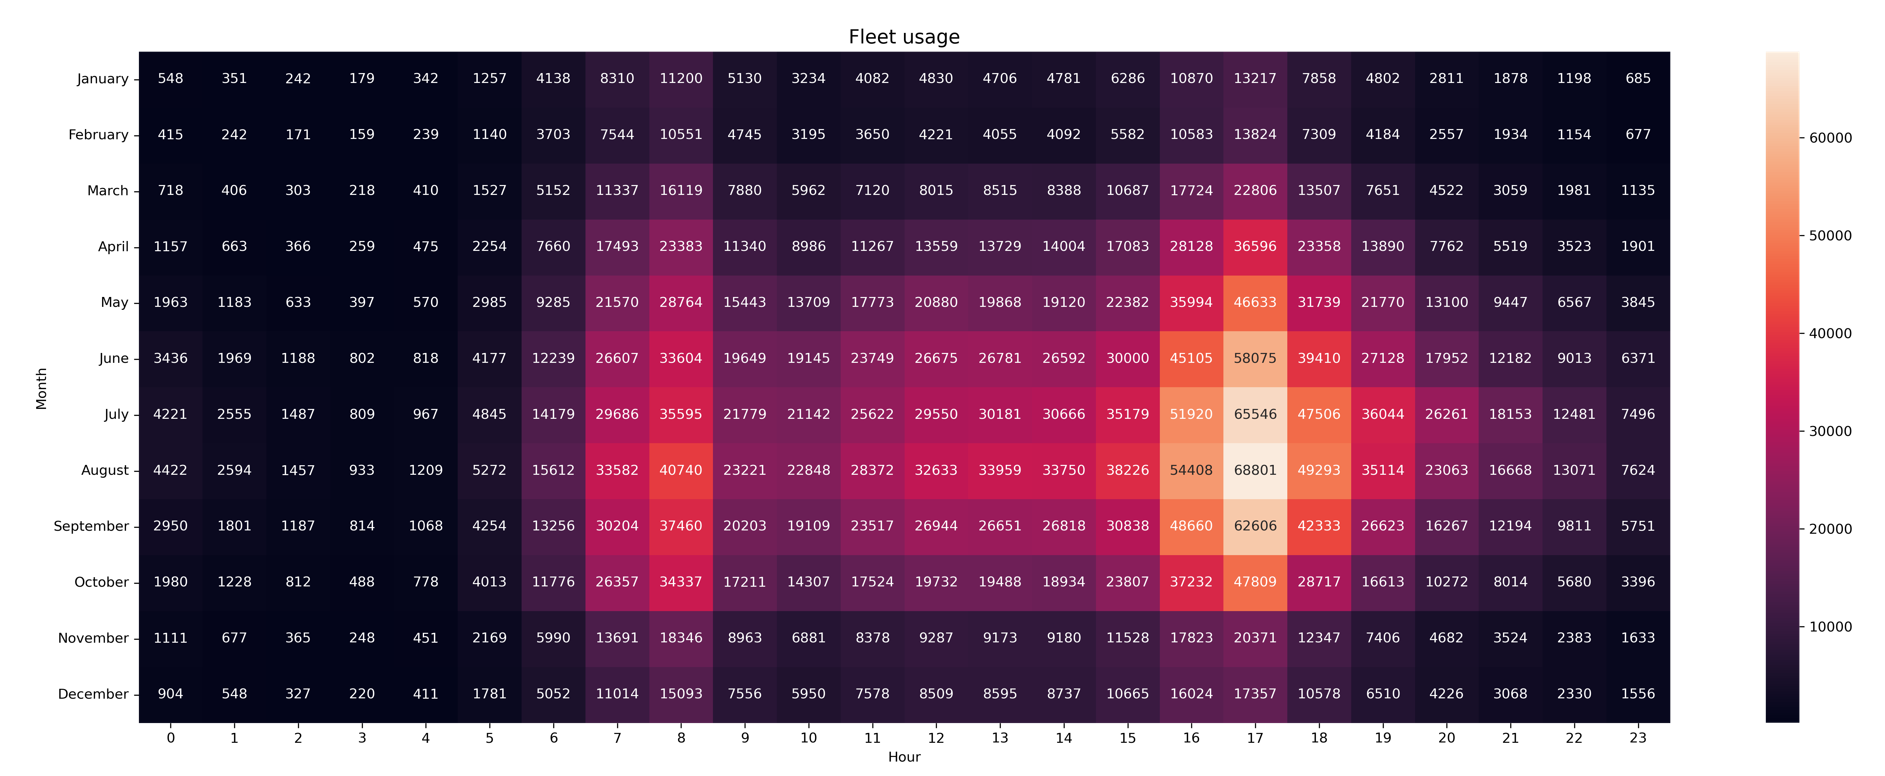
\includegraphics[width=1\linewidth]{./Figures/Usage_Heatmap.png}
    \caption{Fleet Usage}
    \label{heatmap}
\end{figure}

\begin{figure}[H]
    \centering
    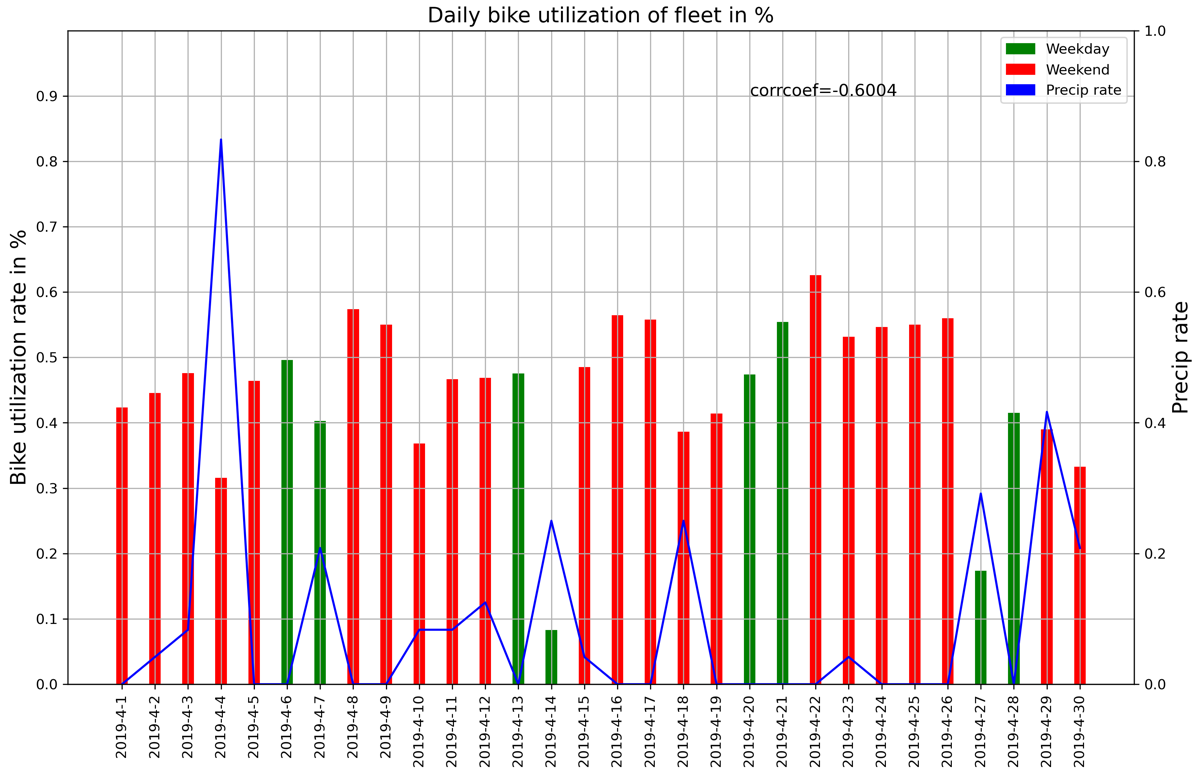
\includegraphics[width=0.7\linewidth]{./Figures/dailyBikeUtilizationApril.png}
    \caption{Daily Bike Utilization of fleet for April}
    \label{dailyBikeUtilizationApril}
\end{figure}

\subsection{Geopraphical Demand Patterns and Top X Stations}
\label{subsec:GeoDemand}

The following section deals with the investigation of the utilization of the individual stations. Several metrics were used to investigate the stations under different perspectives. The first metric we took was to measure the total sum of rides that start and end at each station and to plot the most heavily utilized stations under this definition. 

\begin{figure}[H]
    \centering
    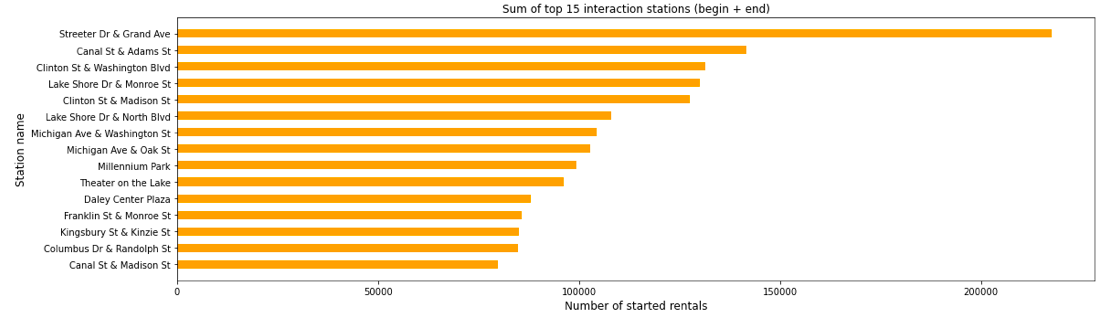
\includegraphics[width=1\linewidth]{./Figures/GeoAbb1.png}
    \caption{Top 15 statitions in terms of starting rides}
    \label{fig1}
\end{figure}


\hyperref[fig1]{Figure 1} illustrates the respective top 15 stations. As can be seen in the plot, the first five stations have a significant lead compared to the place 6 to 15. As a dashboard user, these stations can be seen as most important and should be monitored carefully to avoid longer maintenance. 
Building further upon those 15 stations, a highly skewed distribution of station interactions can be seen in \hyperref[fig4]{Figure 2}. 

\begin{figure}[H]
    \centering
    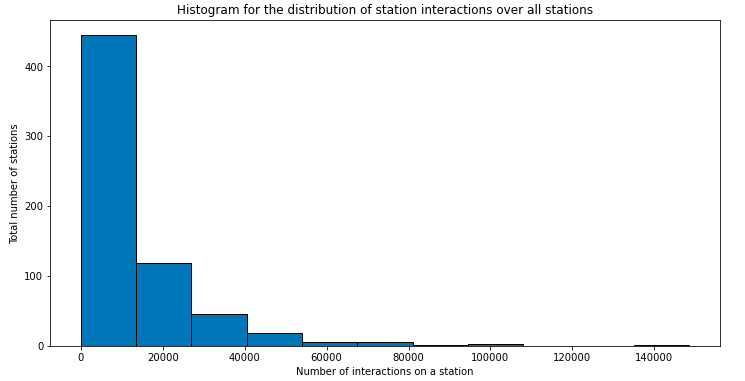
\includegraphics[width=0.7\linewidth]{./Figures/GeoAbb4.png}
    \caption{Histogram for the distribution of station interactions over all stations}
    \label{fig4}
\end{figure}

Most stations only have limited number of interactions. However, the top 50 stations already account for one third of the overall interactions. Also, the 0.75-quantile is very meaningful, stating that 75 percent of all stations have 16,850 or less interactions. Nevertheless, one should not diminish the importance of these stations, as 31 percent of all interactions are represented by them, stating that also the smaller stations are vital for daily business.
Another perspective was taken in \hyperref[fig4]{Figure 3}.

\begin{figure}[H]
    \centering
    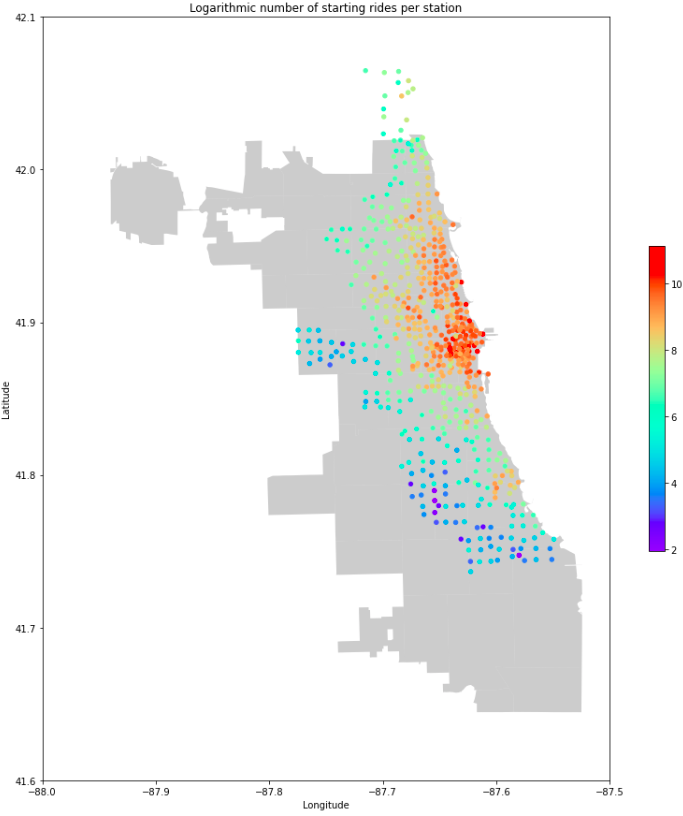
\includegraphics[width=0.6\linewidth]{./Figures/GeoAbb9.png}
    \caption{Logarithmic number of starting rides per station}
    \label{fig9}
\end{figure}


Here, the logarithmic number of starting rides per station is plotted. It can be easily seen that most of the rides start in the center of Chicago and along the coast, whilst moving to the outskirts of the city decreases the density of rides. The data can thus be clustered into three areas: The core of the city, with the most dense network, then the surroundings of that core that are still centrally located in Chicago and lastly, the outskirts, where only minor amounts of rides are started. We will refer to this structure as "three-ring structure" for the rest of this assignment.  


\subsection{KPI 1: RPUB (Rides Per Unique Bike)}
\label{subsec:KPI1}

The first KPI scrutinizes the number of trips per unique bicycle. The definition of "unique bicycle" is defined as follows: All unique bikes used per each day. The KPI is derived from an article by Sven Boor (2019) and an article by Yanocha, Mason, Patlán, Benicchio et al. (2018), although we adapted the KPI by also calculating hourly values, not only daily ones, in order to fulfill the task. The first insight that can be derived is that a clear seasonality can be exhibited with the highest values during summer and the lowest during winter \hyperref[kpi1abb1]{Figure X}.

\begin{figure}[H]
    \centering
    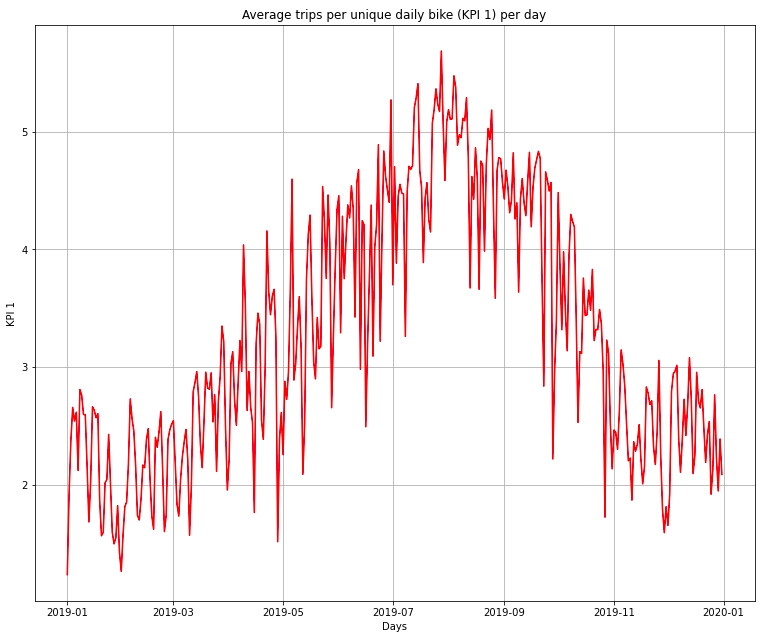
\includegraphics[width=0.7\linewidth]{./Figures/kpi1abb1.png}
    \caption{Average trips per unique daily bike (KPI 1) per day}
    \label{kpi1abb1}
\end{figure}

RPUB based on unique daily bikes always lies within the interval defined by Boor (2019) of 4-8 trips per bike. During summer, it averages around a value of 5, which is fine, however during winter, spring and autumn, it falls below the lower boundary of 4 defined by Boor (2019). This could indicate that the number of bikes during winter is too high.

\begin{figure}[H]
   \centering
    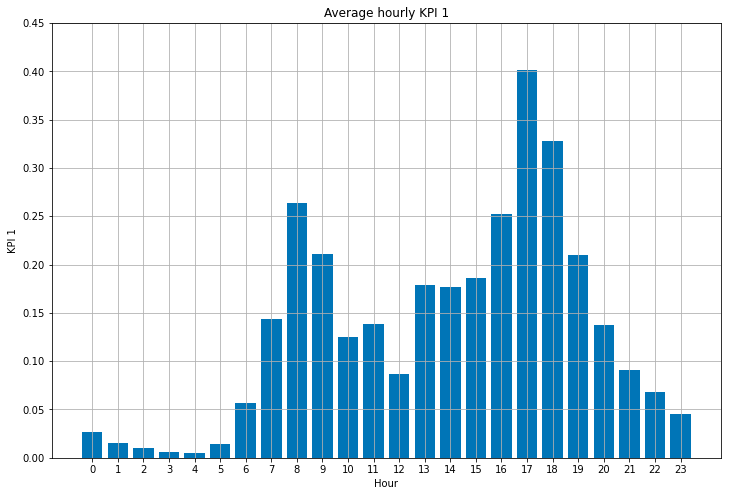
\includegraphics[width=0.7\linewidth]{./Figures/kpi1abb3.png}
    \caption{Average hourly KPI 1}
    \label{kpi1abb3}
\end{figure}

When looking at the hourly RPUB values averaged over the entire year \hyperref[kpi1abb3]{Figure X}, a very explicit commuter pattern can be observed, as the values peak at around 8 and 17 o' clock. Interestingly, at 5 o'clock, the KPI stands at around 0.4, which is more than twice as high than the average monthly value in July, the most "active" month. A bike at that time performs around 0.4 rides per hour. Thus, commuting activity has a tremendous impact on the utilization of the divyy system, much more than monthly seasonality.
Comparing weekend and weekdays hourly \hyperref[kpi1abb5]{Figure X}, it becomes clear that the weekend RPUB values are not higher or lower than the weekday ones, except for the situation during noon and at around 9/17 o' clock. Thus, it can again be reasoned that commuting is a significant driver of the divyy bike system and peak around noon due to leisure activities. As the influence of the weather data was insignificant, it can be consulted in the \hyperref[APP1]{Appendix}.

\begin{figure}[H]
   \centering
    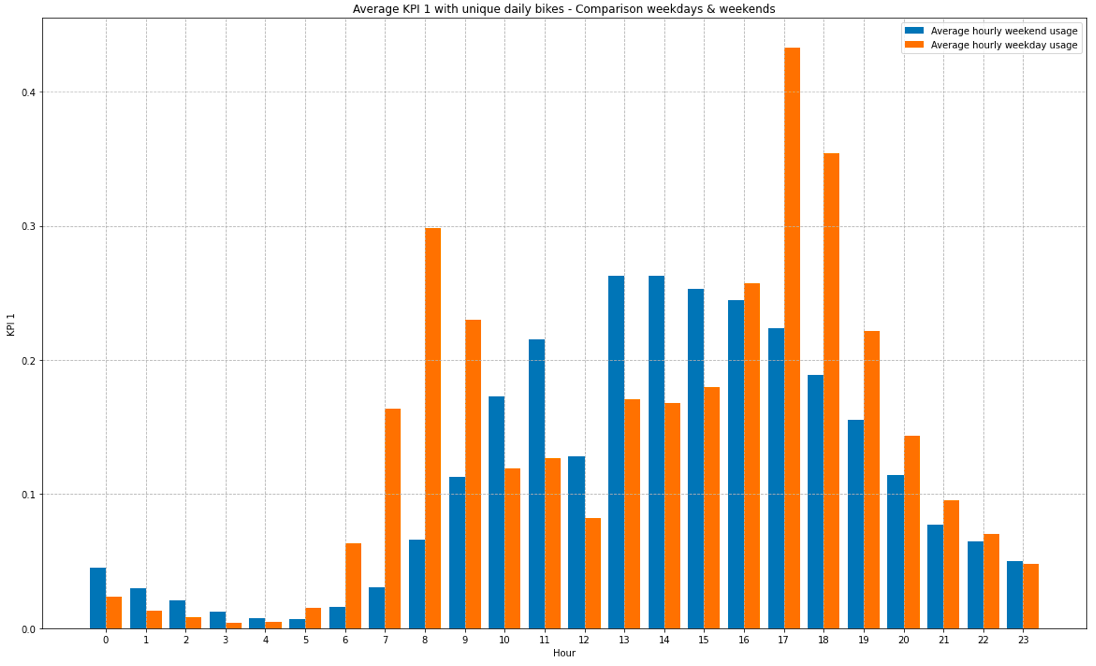
\includegraphics[width=0.7\linewidth]{./Figures/kpi1abb5.png}
    \caption{Average KPI 1 with unique daily bikes - Comparison weekdays & weekends}
    \label{kpi1abb5}
\end{figure}

\subsection{KPI 2: Demand-Capacity}
\label{subsec:KPI2}

This KPI is related to "coverage". The KPI should investigate whether the distribution and the number of stations is sufficient. Demand-Capacity divides the maximum of the number of arriving and departing rides per hour per station by the capacity in terms of how many bikes that station can hold. For further explanation, refer to the Jupyter notebook. For \hyperref[kpi2abb1]{Figure X}, it was counted how many rides were started at a station exhibiting high Demand-Capacity values (category 3) or mediocre/low (category 2 and 1) values. 

\begin{figure}[H]
   \centering
    \includegraphics[width=0.6\linewidth]{./Figures/kpi2abb1.png}
    \caption{Maximum Utilization Category Count}
    \label{kpi2abb1}
\end{figure}

As can be clearly seen, the number of rides starting at a category three station is very low. A similar notion arises when investigating the average Demand-Capacity value per month \hyperref[kpi2abb2]{Figure X}.

Moreover, when investigating the average hourly Demand-Capacity value (\hyperref[kpi2abb3]{Figure X}, whilst a commuting pattern can be observed similar to that of RPUB, even during the most industrious time of 17 o'clock, the KPI does not exceed an average value of 0.4. 

Splitting the same hourly illustration into summer and winter values \hyperref[kpi2abb4]{(Figure X)}, the value peaks at around 0.4. This notion does not change when distinguishing the hourly values in terms of weekday vs weekend \hyperref[kpi2abb5]{(Figure X)}. Interestingly, the values peak at 5 pm at just below 0.35, whilst the maximum was around 0.4 during summer. Thus, the season has a higher influence on the Demand-Capacity than time alone.

\begin{figure}[H]
  \centering
  \subfloat[Comparison summer and winter]{\includegraphics[width=0.5\textwidth]{./Figures/kpi2abb4.png}\label{fig:f1}}
  \hfill
  \subfloat[Comparison weekdays and weekends]{\includegraphics[width=0.5\textwidth]{./Figures/kpi2abb5.png}\label{fig:f2}}
  \caption{Average KPI 2 value per hour}
\end{figure}

In order to investigate stations that exhibit problematic behavior in terms of the Demand-Capacity, we limited the data to the 20 most "problematic" stations, that is, the stations that exceeded a Demand-Capacity value of 1 most often. Investigating those 20 stations, it can be seen (\hyperref[kpi2abb6]{(Figure X)} that during non-summer months, the Demand-Capacity values are not problematic, as they rarely exceed a value of 0.4. However, during summer, the upper boundary of the standard-deviation intervals exceeds values of up to 1.4, which can be considered problematic.

\begin{figure}[H]
   \centering
    \includegraphics[width=0.75\linewidth]{./Figures/kpi2abb6.png}
    \caption{The average maximum KPI 2 value per day of the 20 most utilized stations with standard deviation}
    \label{kpi2abb6}
\end{figure}

\subsection{KPI 3: Average Rental Durations}
\label{subsec:KPI3}

As a next KPI, the average hourly rental durations over different aggregated time slots were observed in order to get a detailed insight on different patterns. The main key aspects we drew from that analysis are described in the following. First, there is a common pattern that the longest duration rides occur between 10am and 5pm, so during the midday the average duration is the highest. Between 12am and 4am, the average hourly duration is at its second-highest peak. Between 5 am and 9 am, the average duration is lowest during the day, meaning that those bike rides are more often used for short trips. This pattern is visualized in \hyperref[Duration_Fig_1]{Figure 13}, whereby the pattern did not only occur on an aggregation level over the whole year but also in summer, winter, weekends and weekdays. Next, different aggregation levels were analyzed, and the final results can be seen in Appendix \hyperref[Duration_Fig_2]{ Figure 14}. Again, a seasonality pattern can be observed, in which in summer longer durations occur than in winter. Additionally, durations on weekends in summer are on average 5 minutes longer than on weekdays and in winter there are overall shorter durations during the entire day regardless of weekend or weekday. Furthermore, a weather pattern can be observed which tells us that during precip, the average durations are usually shorter while during warmer temperature they are longer.

\begin{figure}[H]
   \centering
    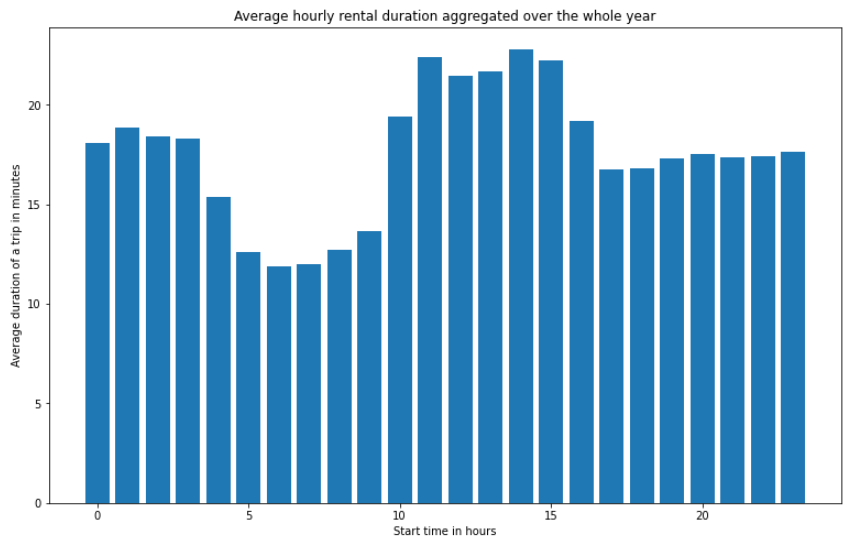
\includegraphics[width=0.8\linewidth]{./Figures/Duration_Fig_1.png}
    \caption{Average hourly rental duration aggregated over the whole year}
    \label{Duration_Fig_1}
\end{figure}

\subsection{KPI 4: Revenue}
\label{subsec:KPI4}

The revenue is the last KPI. The total revenue excluding subscriptions is 4656803 Dollar including subscriptions 8652803 Dollar \hyperref[fig_revenue_1]{(Figure 6)}. The revenue from subscribers can only be estimated, because they pay an annual subscription and we have not the number of subscribers nor the user IDs to calculate the numbers \hyperref[fig_revenue_1]{(Figure 6)}. The revenue from customers is directly depending on the number of trips from customers. Also, it is depending on the duration of the trips for both types of users as trips longer than 30 (customer) /45 minutes (subscriber) are paid by minute. Thus, the patterns observed for the usage of bike fleet and duration of trips apply to the revenue. The revenue from customers is volatile and peaks in summer while the revenue from the subscriptions is quite stable \hyperref[fig_revenue_2]{(Appendix Figure 7)}. Also, the mean revenue per trip is higher in summer than in winter due to the longer duration of trips in mean lead back to the weather. The mean revenue per trip per day is highest on the weekend \hyperref[fig_revenue_3]{(Appendix Figure 8)}. 

\begin{figure}[H]
    \centering
    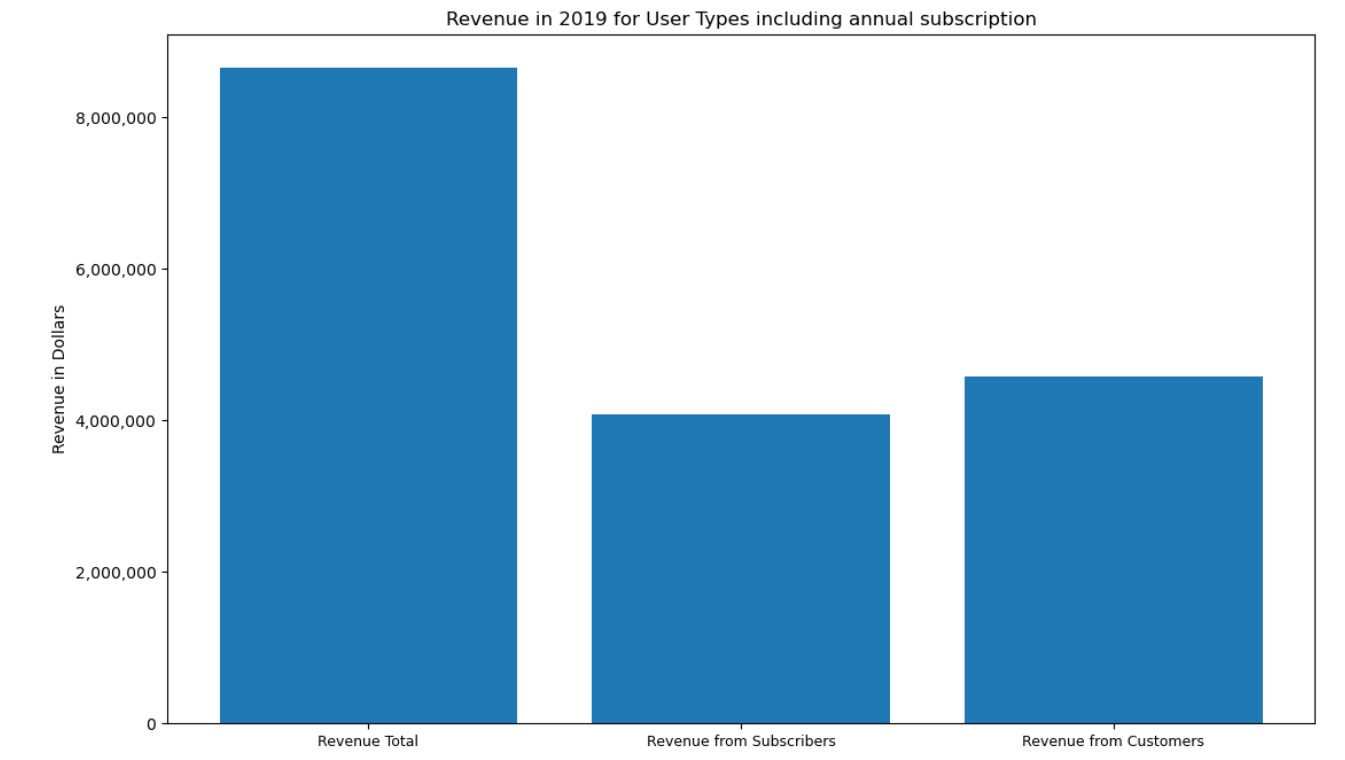
\includegraphics[width=0.7\linewidth]{./Figures/Revenue_annual.jpeg}
    \caption{Revenue in 2019 for User Types including annual subscription}
    \label{fig_revenue_1}
\end{figure}


\section{Data Analytics}
\label{sec:Data Analytics}

\subsection{Cluster Analysis}
\label{subsec:clustering}
Firstly, we will create clusters based on trip durations, weather (temperatures and precip) and revenue characteristics as described and calculated in the descriptive section. Thus, we develop station-related clusters and transaction-related clusters. Secondly, we will try to develop clusters of stations based on activity measures (KPI2, number of starting rides per station).
During clustering, we would like to refer to the mean duration of each available hour to one ‘trip’. The application of K-Means as a hard clustering method and the Gaussian Mixture model as soft clustering method results in three reasonable clusters describing duration as a single input feature.  The number of clusters is derived from the elbow point and silhouette scores, visualized in \hyperref[LossKMeans_Duration_dpi300]{Appednix Figure X} and \hyperref[Silhouette_Duration]{Appendix Figure X}. The visualization of the clusters reveals short trips (<14 min.), medium trips (<24 min.) and long trips (>24 min.) (\hyperref[FINAL_Clusters_Duration]{Figure X}). The Gaussian Mixture model result suggests, instead of a cluster for long trips, a cluster for extreme trips, which includes both very short and long trips (\hyperref[FINAL_Cluster_Gaussian_Duration]{Appendix Figure X}). 

\begin{figure}[H]
   \centering
    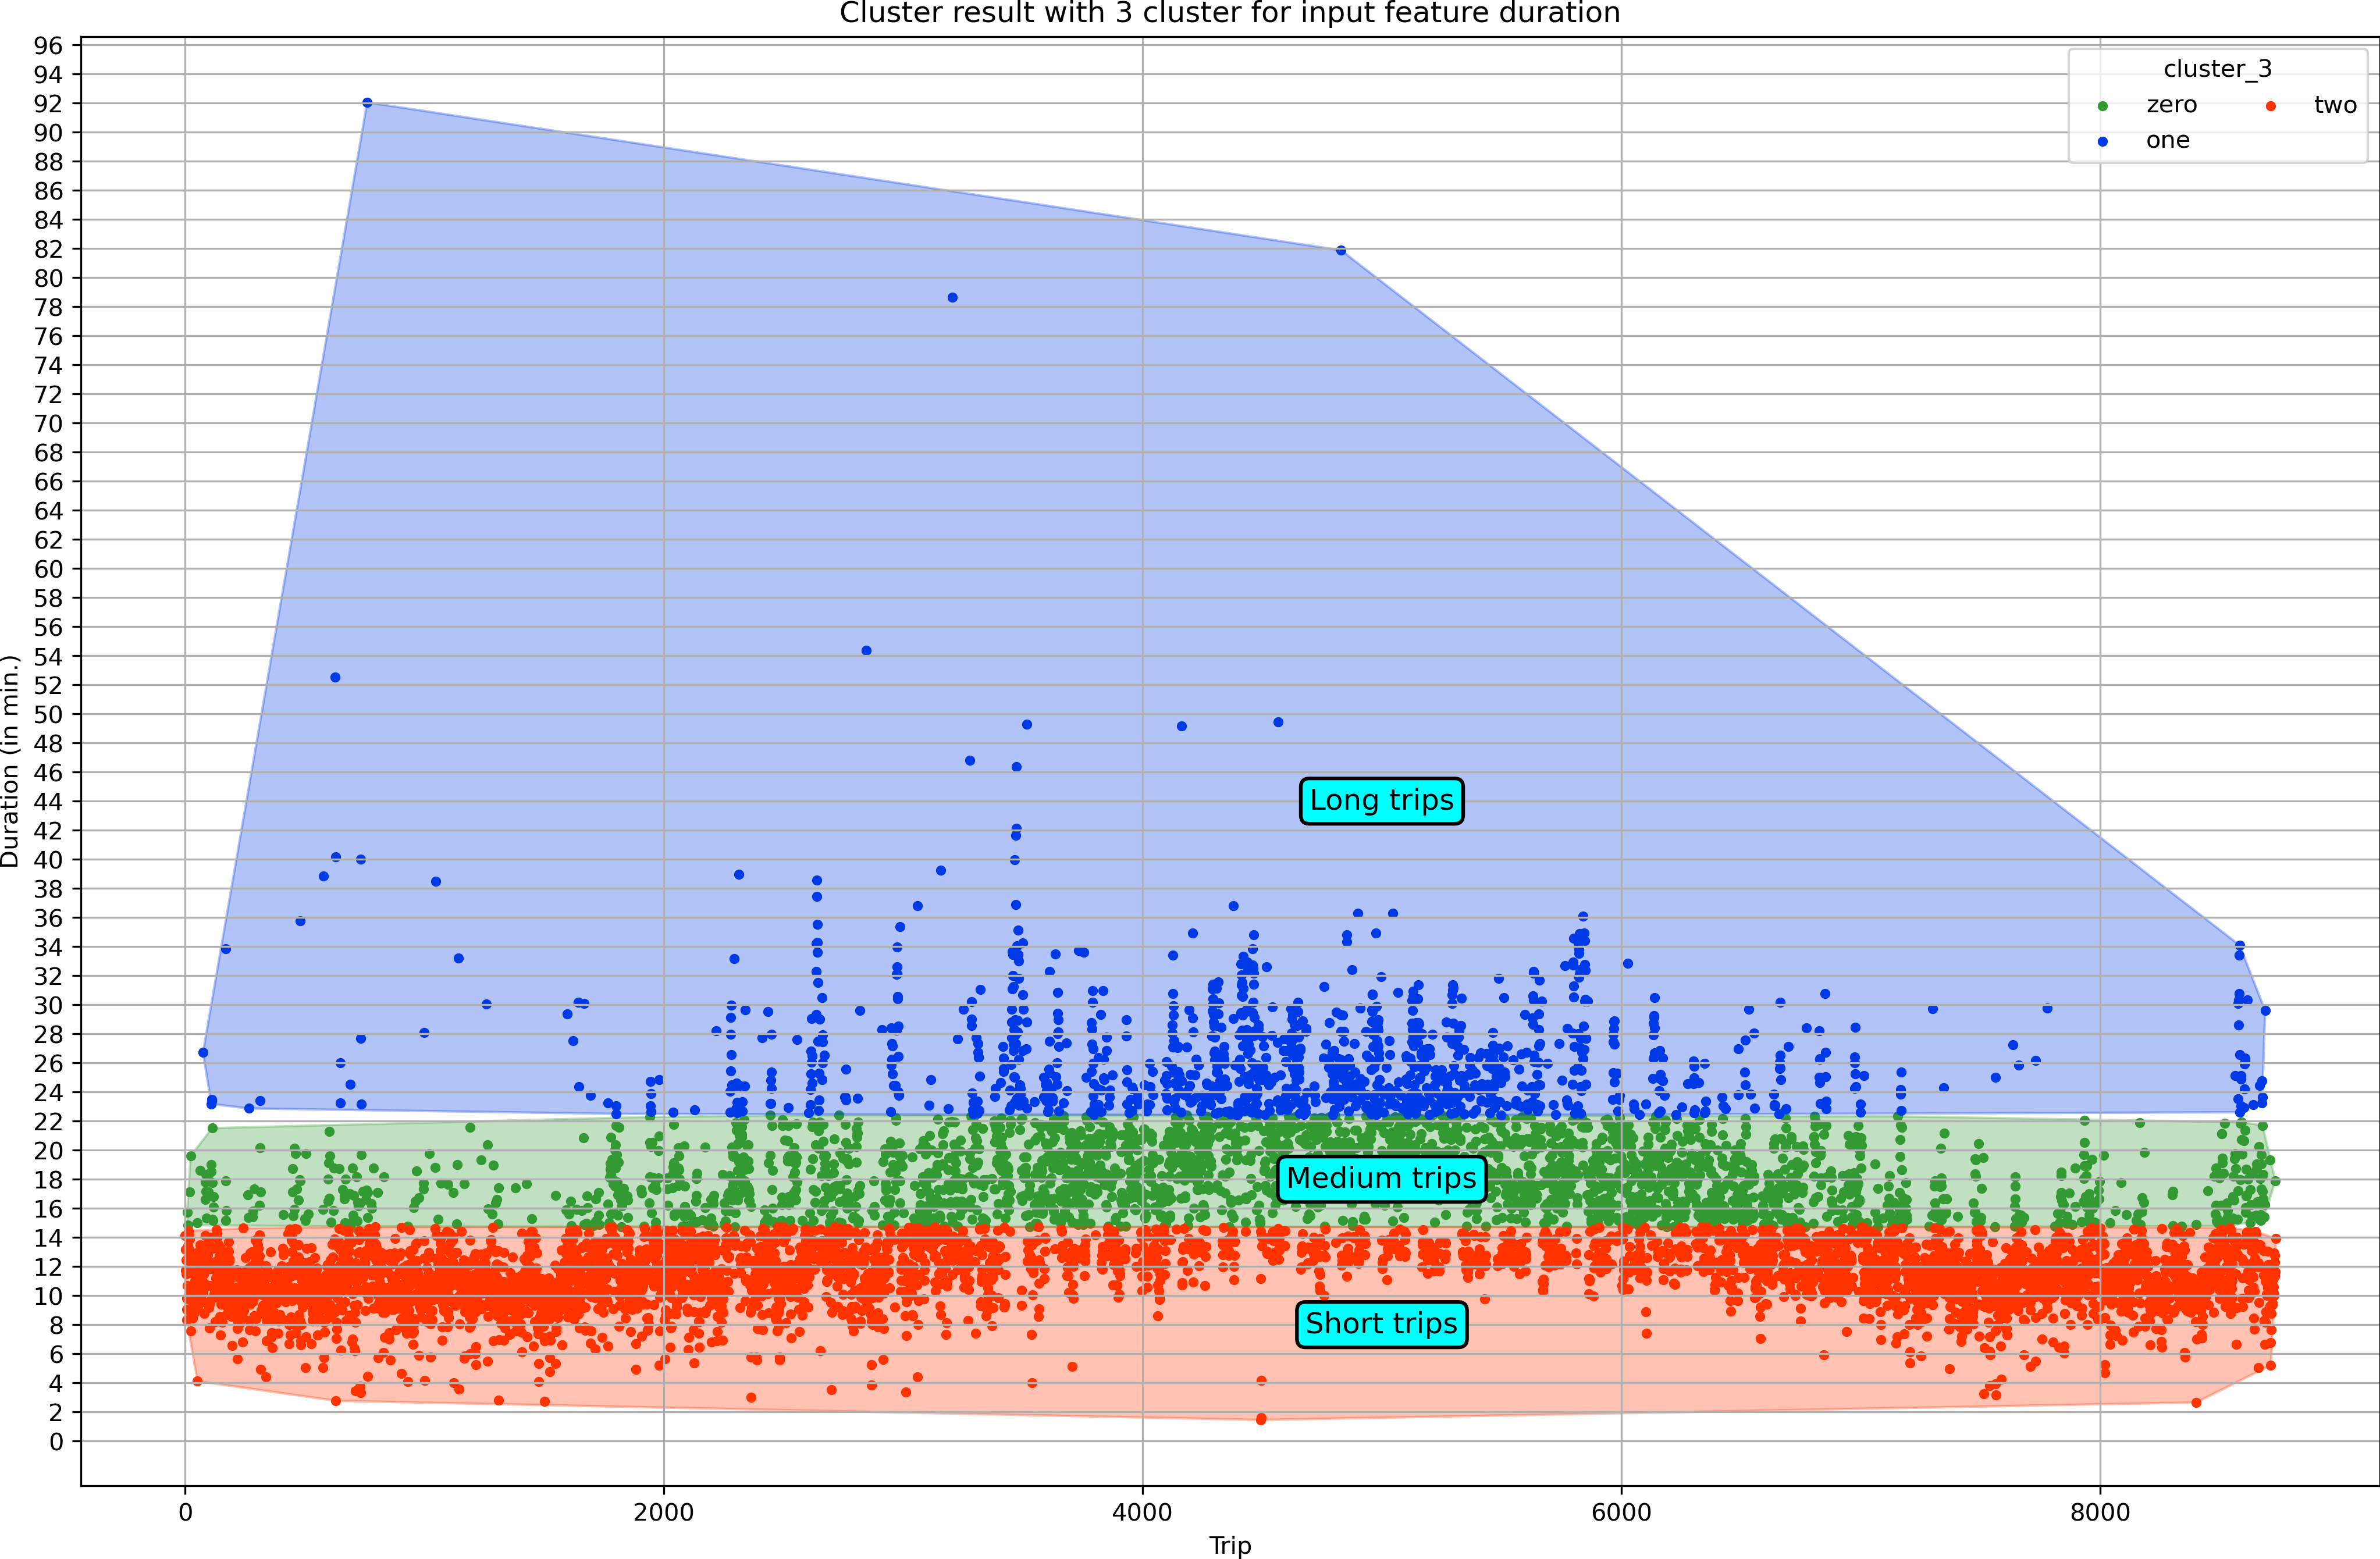
\includegraphics[width=0.75\linewidth]{./Figures/FINAL_Clusters_Duration.png}
    \caption{Cluster result with 3 cluster for input feature duration}
    \label{FINAL_Clusters_Duration}
\end{figure}

The clustering with duration and temperature lead to six differentiations, visualized in \hyperref[FINAL_Cluster_KMEANS_Duration_Temp]{Figure X}. Following the elbow method (\hyperref[Loss_Duration_Temp]{Appendix Figure X}), one would choose the cluster result with 3 clusters (\hyperref[Cluster_KMEANS_Duration_Temp]{Appendix Figure X}), but this cluster assignment seems too superficial and does not represent the different combined intervals of duration and temperature values in an adequate manner. The Gaussian model adds a new perspective, as the data is now largely represented by elliptical cluster structures. The clusters leave a large scope for interpretation and are highly subjective. Despite the better coverage of elliptical structures, a more reasonable classification as with K-Means cannot be found (\hyperref[Silhouette_Gaussian_Duration_Temp]{Appendix Figure X} and \hyperref[Clusters_Gaussian_Duration_Temp]{Appendix Figure X}).

\begin{figure}[H]
   \centering
    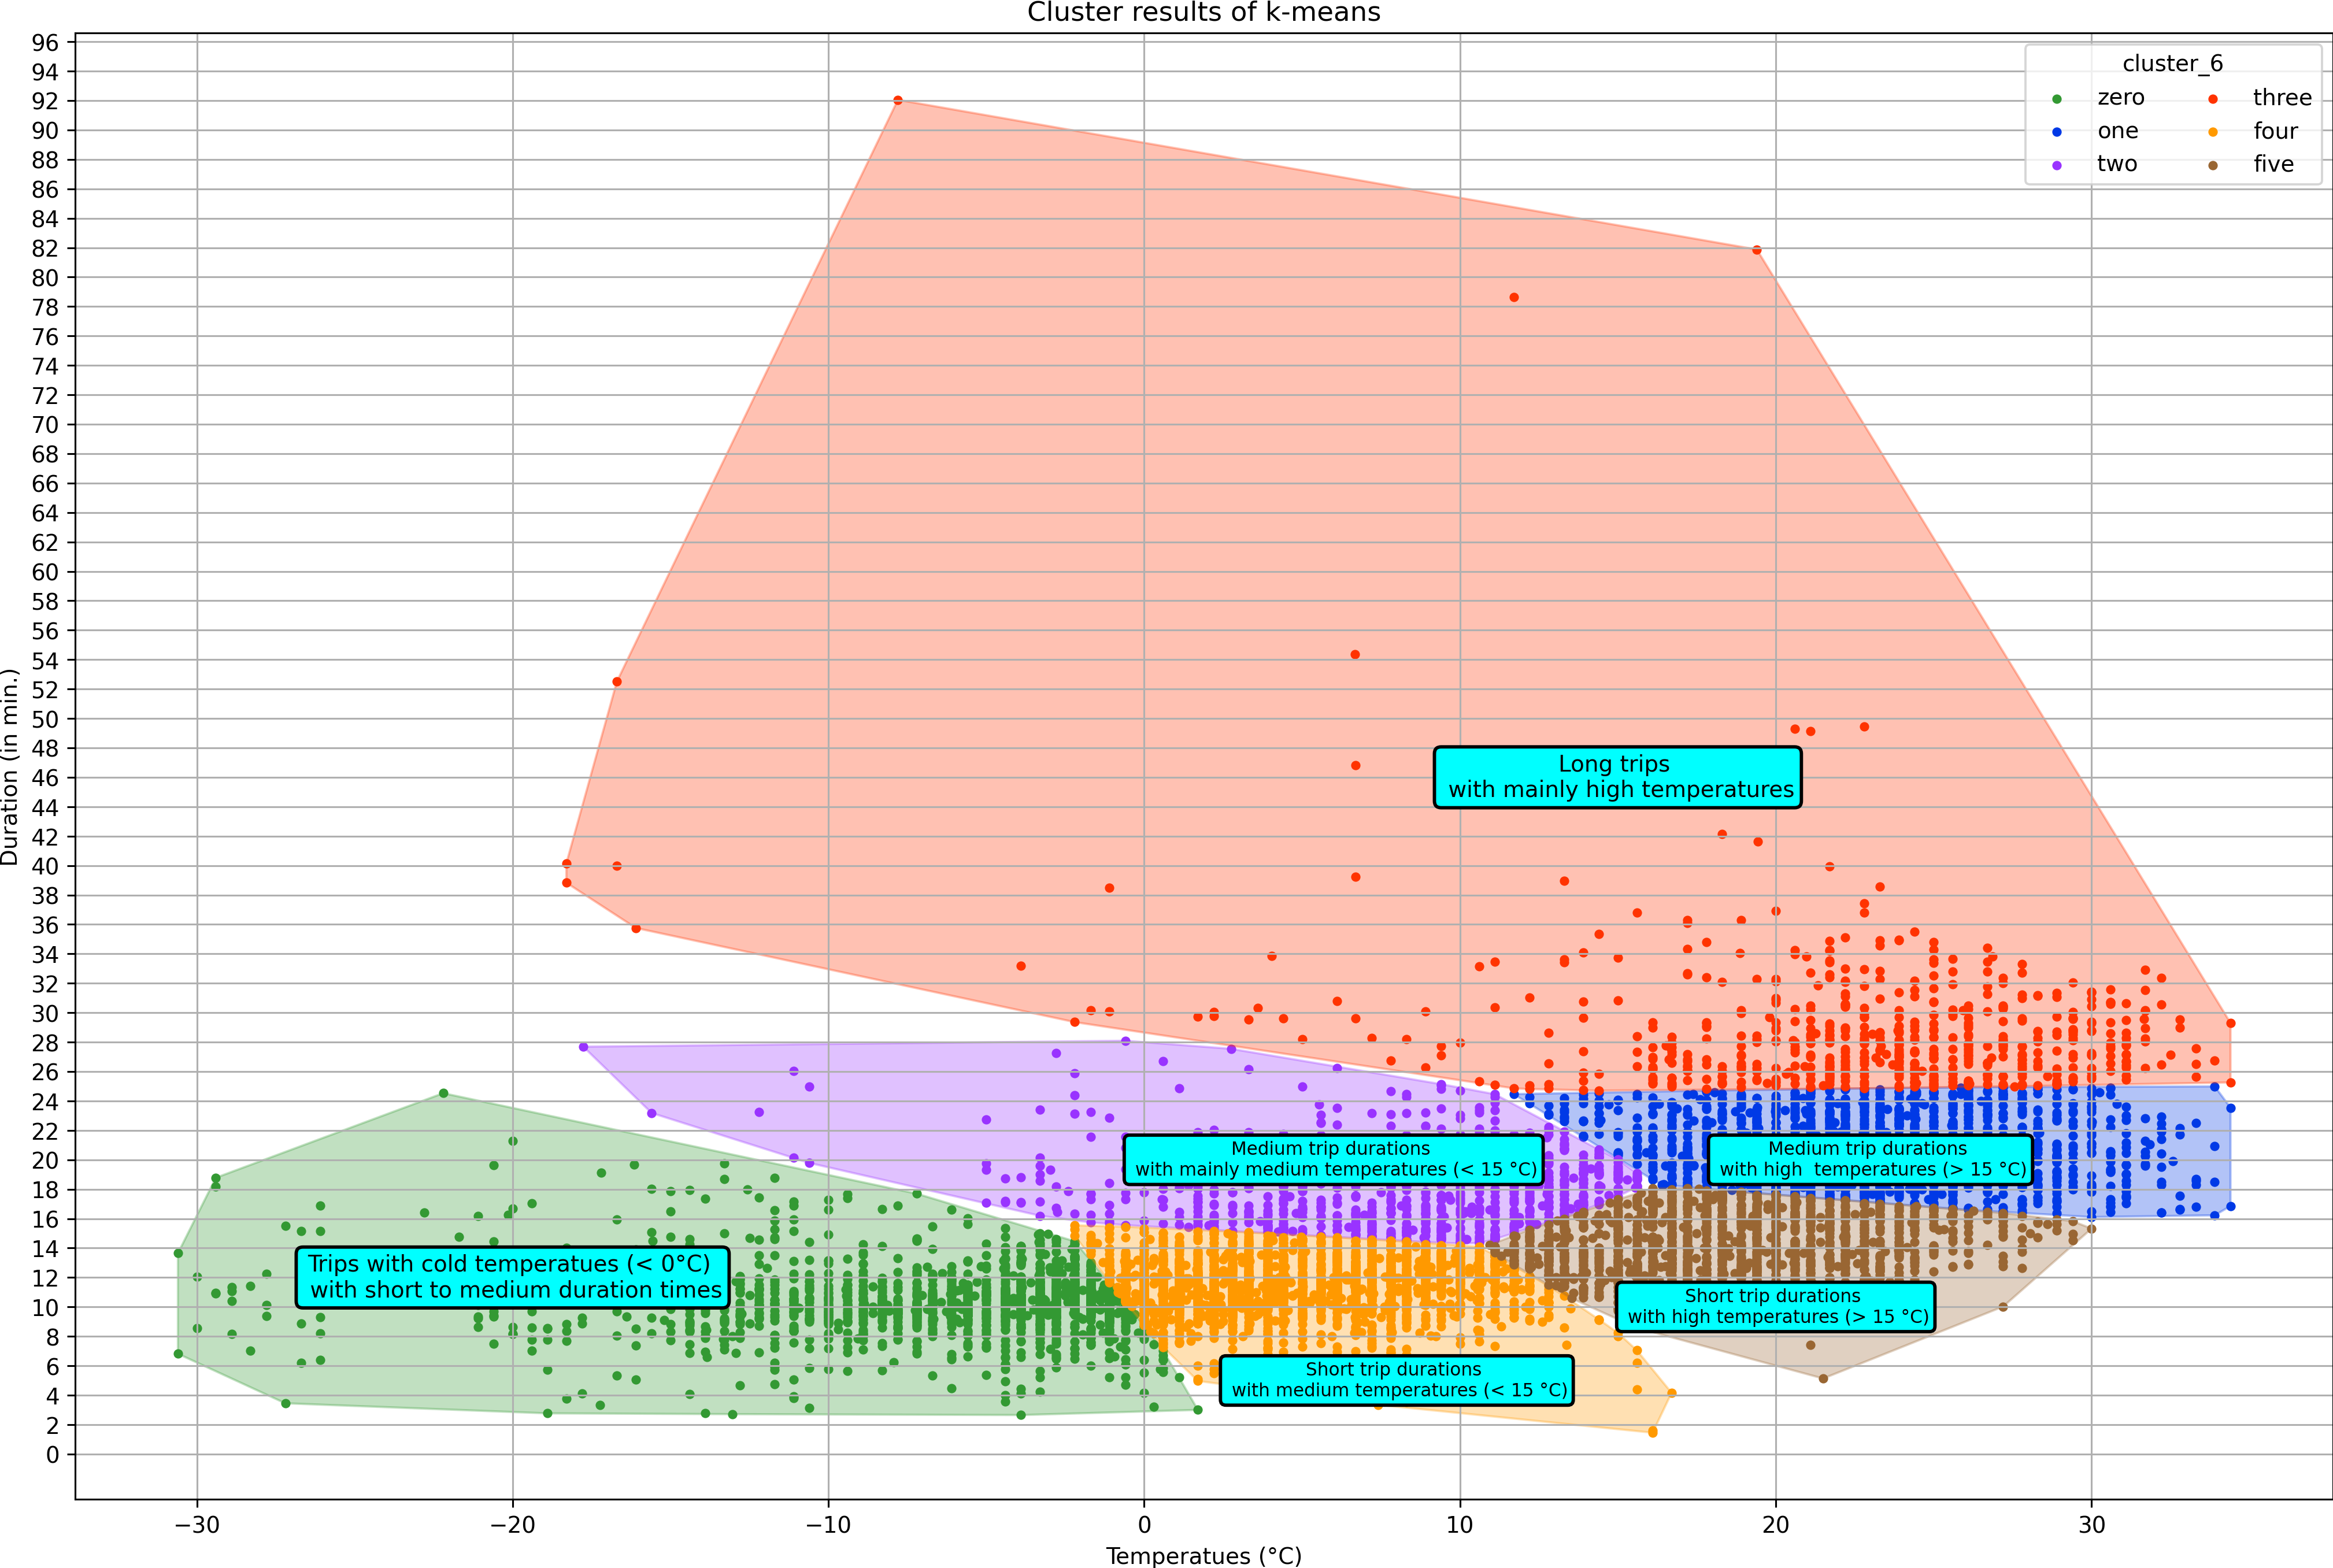
\includegraphics[width=0.8\linewidth]{./Figures/FINAL_Cluster_KMEANS_Duration_Temp.png}
    \caption{Cluster result K-Means}
    \label{FINAL_Cluster_KMEANS_Duration_Temp}
\end{figure}

Taking precip into account, the complementary cluster to the K-Means result with 6 cluster is visualized in \hyperref[FINAL_Cluster_Duration_Temp_Precip]{Figure X}. The K-Means algorithm found the same 6 clusters, but additionally differentiate rain trips by adding two rain clusters.\\

\begin{figure}[H]
   \centering
    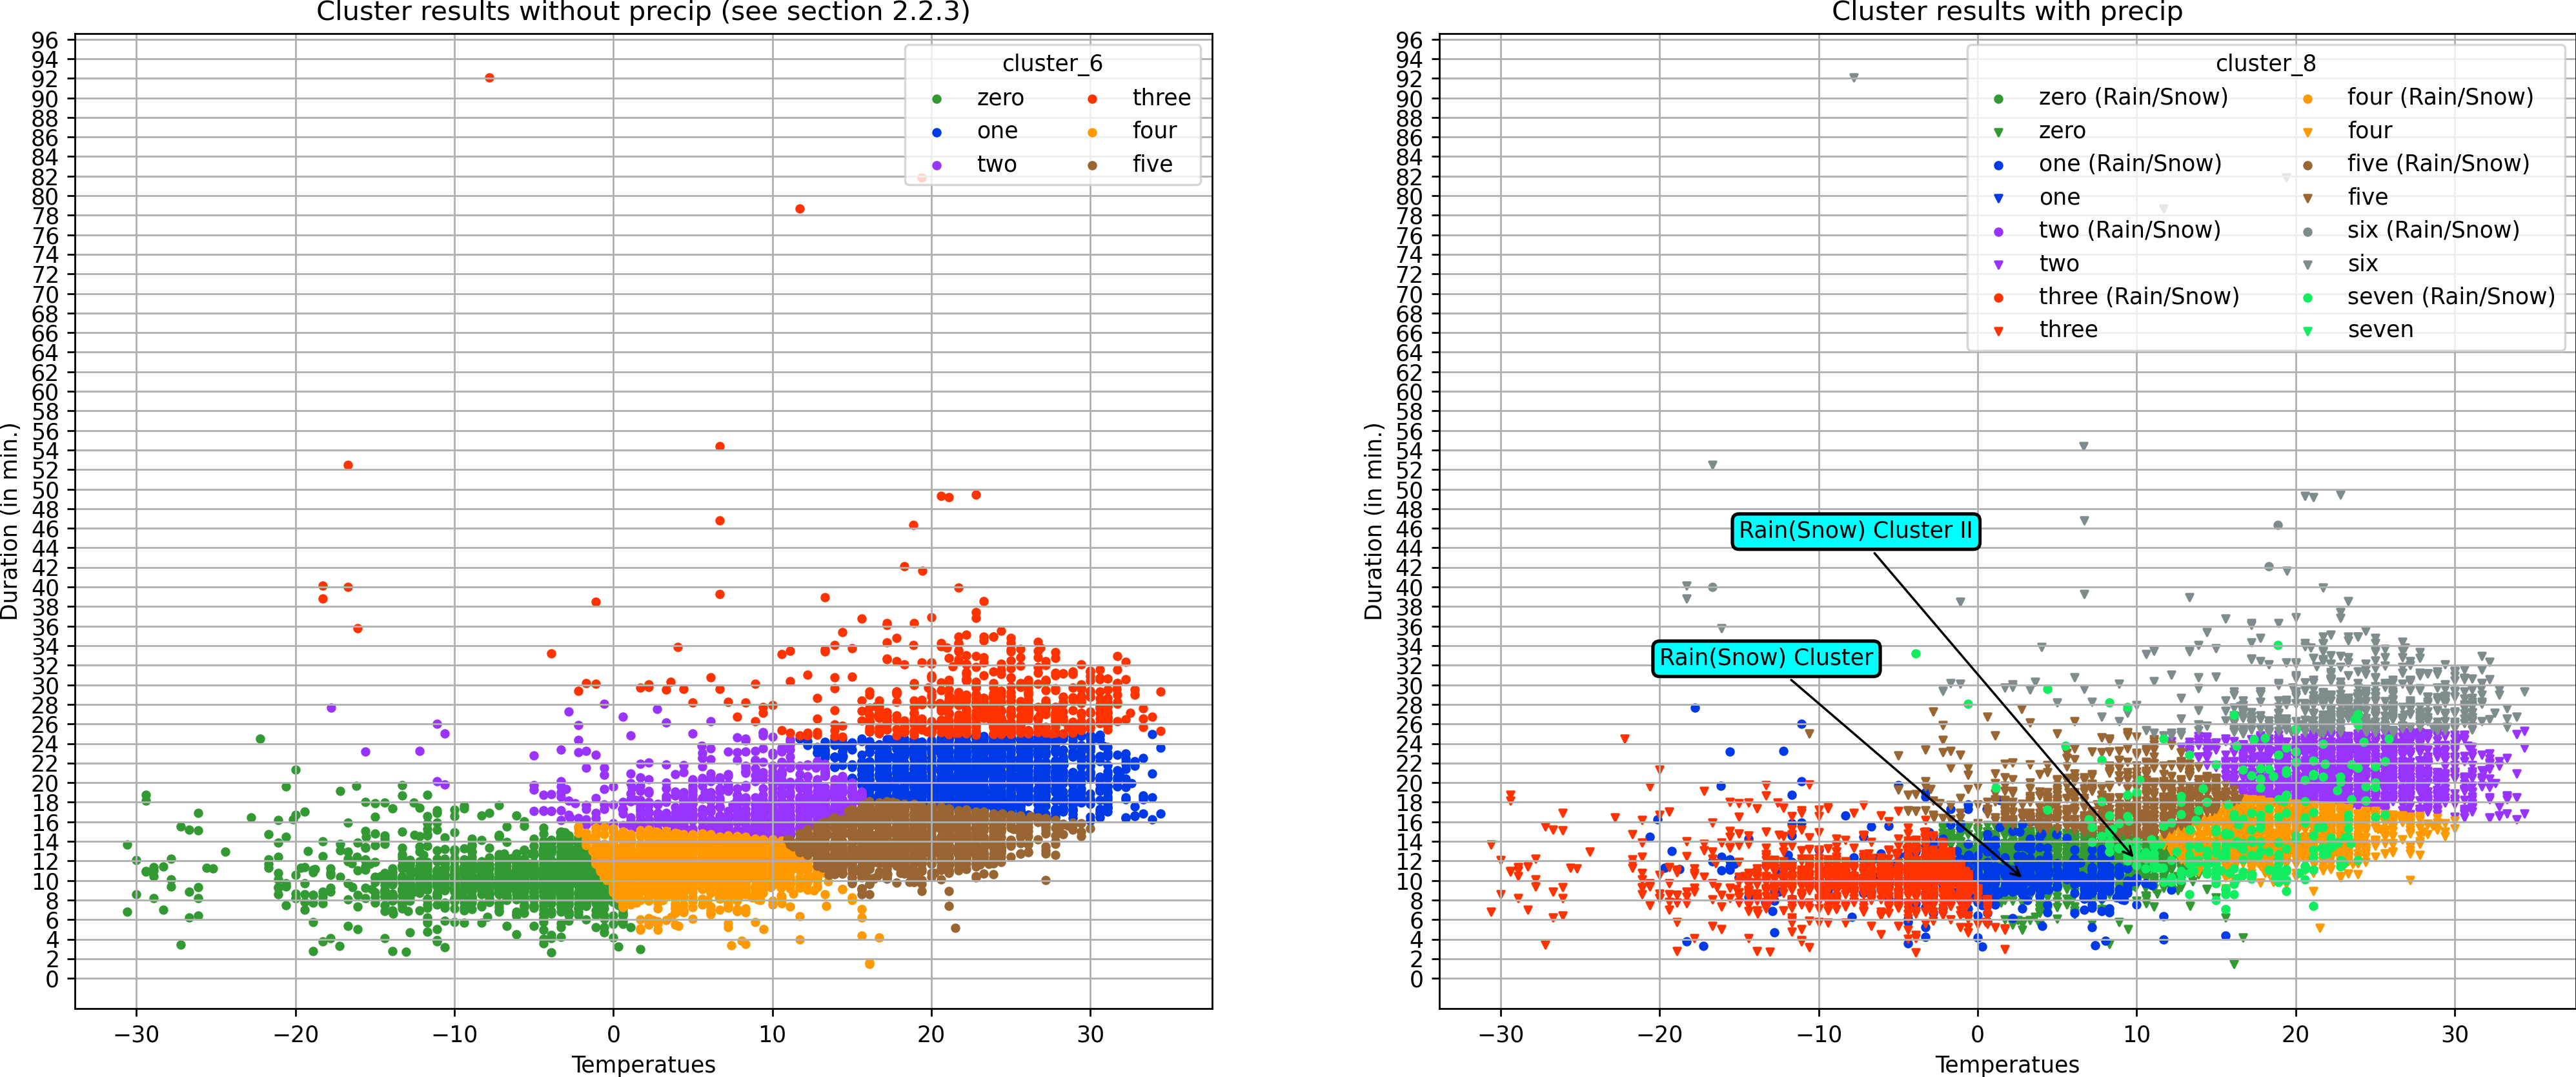
\includegraphics[width=1\linewidth]{./Figures/FINAL_Cluster_Duration_Temp_Precip.png}
    \caption{Cluster result K-Means with and without precip}
    \label{FINAL_Cluster_Duration_Temp_Precip}
\end{figure}

We decided to cluster the revenue hourly (averaged) to yield a reasonable amount of data with K-Means and GMM. The Silhouette Score for the latter one \hyperref[BCABB1]{( Appendix Figure X)} indicates that three clusters are optimal.
The results of the K-Means are found in (\hyperref[BCAPP1]{Appendix X} and \hyperref[BCAPP2]{X}). We found the GMM clusters to be more reasonable, thus we continued to work with those (\hyperref[BCABB2]{Figure X}). 

\begin{figure}[H]
   \centering
    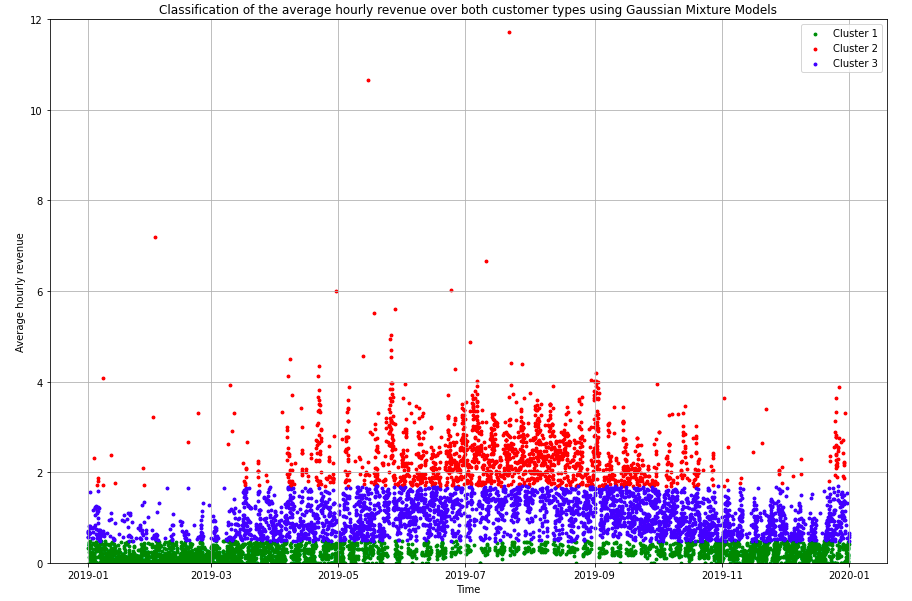
\includegraphics[width=0.8\linewidth]{./Figures/BC_ABB2.png}
    \caption{Classification of the average hourly revenue over both customer types using Gaussian Mixture Models}
    \label{BCABB2}
\end{figure}

Looking at the monthly share of revenue per cluster (\hyperref[BCABB3]{Figure X}), it is evident that during winter, autumn and spring, usually the blue cluster accounts for most of the revenue, although in January and February, the share of the green cluster is nearly equally high. During summer however, especially in July and August, the red cluster accounts for the absolute majority of the revenue, indicating the importance of long rides during the warm summer months for the ride sharing system. Adding the average hourly temperature as input feature does not yield relevant insights, which is described in (\hyperref[BCAPP5]{Appendix X - X}).

\begin{figure}[H]
   \centering
    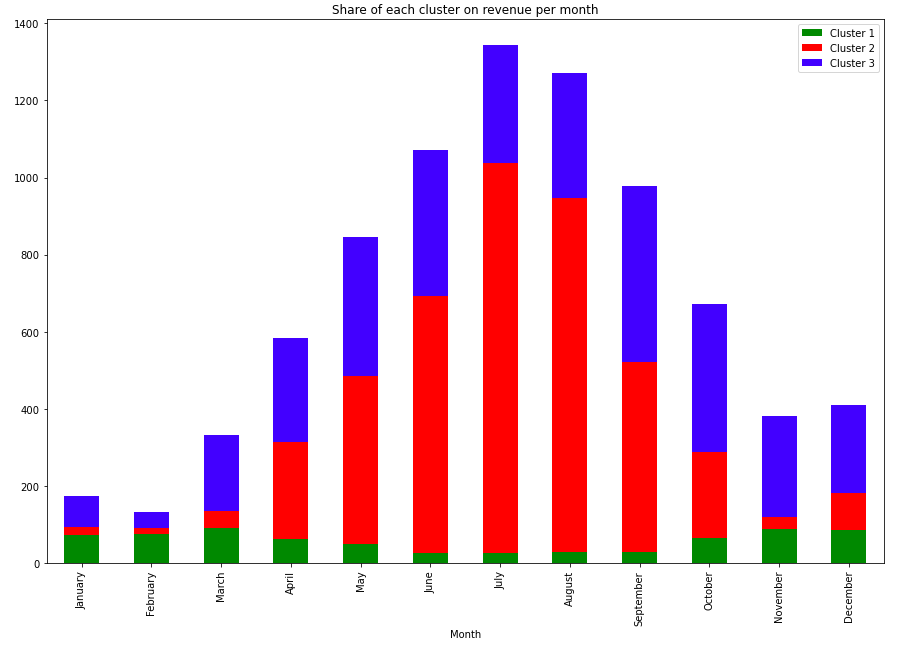
\includegraphics[width=0.65\linewidth]{./Figures/BC_ABB3.png}
    \caption{Share of each cluster on revenue per month}
    \label{BCABB3}
\end{figure}

Now, the individual stations were clustered, beginning with the Demand-Capacity (see the descriptive part for the explanation) as the sole input feature. Applying K-Means and again using the elbow-method (\hyperref[BCABB7]{Appendix Figure X}) does not yield a clear optimal number of clusters, however we discovered a clear three-ring structure in the descriptive analysis and thus chose three clusters. 

\begin{figure}[H]
   \centering
    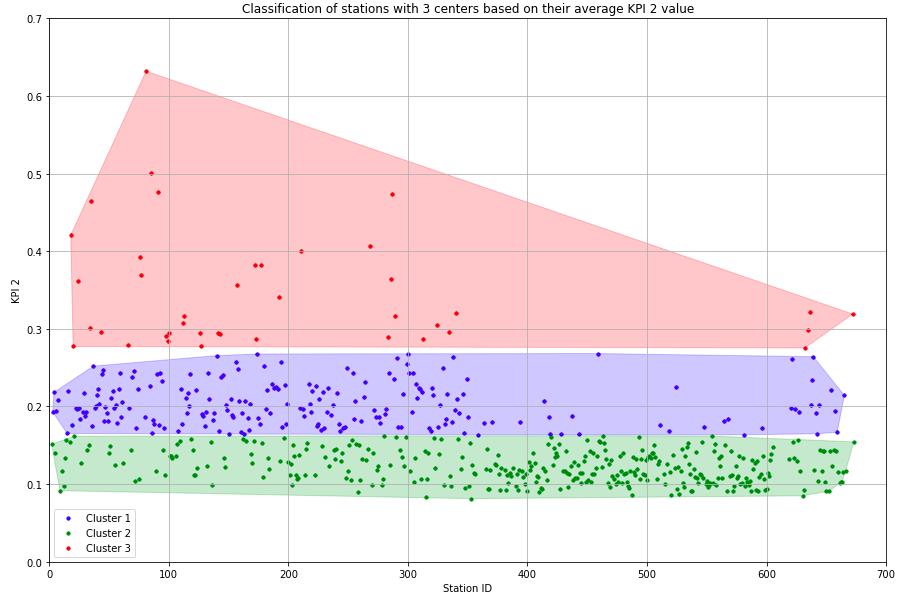
\includegraphics[width=0.8\linewidth]{./Figures/BC_ABB8.png}
    \caption{Classification of stations with 3 centers based on their average KPI2 value}
    \label{BCABB8}
\end{figure}

\begin{figure}[H]
   \centering
    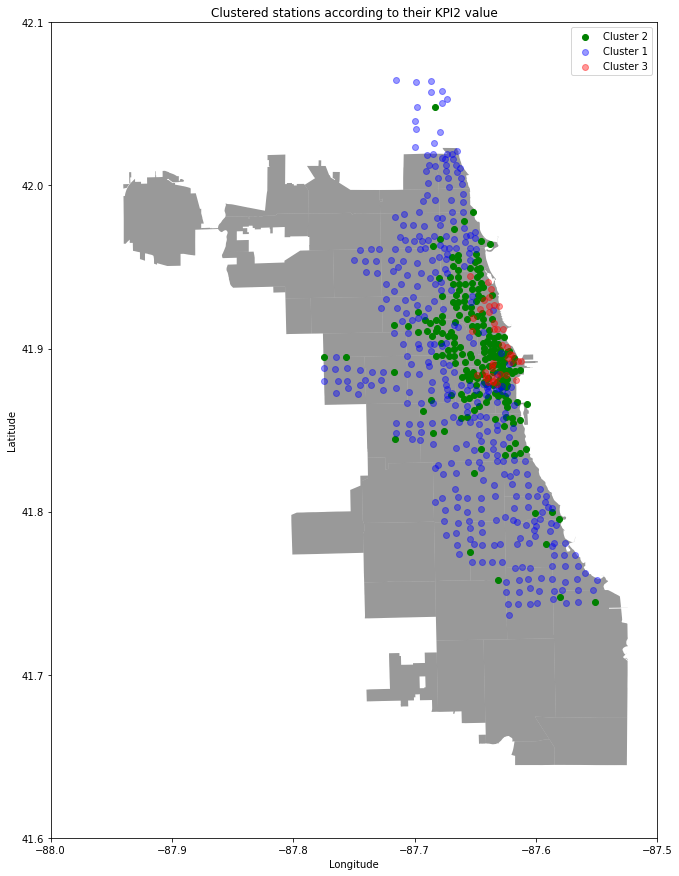
\includegraphics[width=0.75\linewidth]{./Figures/BC_ABB9.png}
    \caption{Clustered stations according to their KPI2 value}
    \label{BCABB9}
\end{figure}

(\hyperref[BCABB8]{Figure X}) illustrates the clusters and serves only as a supporting graph to understand the mapped values (\hyperref[BCABB9]{Figure X}). Here, we can clearly observe the above-mentioned three-ring-structure. Comparing the sketch map in the notebook with a Google Maps representation of Chicago, it gets clear that the majority of the red stations are located near recreational areas close to lake Michigan. A second smaller cluster of red stations seems to be located in downtown/roughly north to the University of Illinois/Chicago. We deduce the following hypothesis: The red stations comprise mainly leisure stations, that are used for recreational purposes. This is backed by the figure in  (\hyperref[BCABB10]{Figure X}), where the “red” Demand-Capacity development is largely season dependent - this makes sense, as during summer, there are obviously more rides related to recreational purposes. The blue and green cluster cannot be significantly distinguished. Several other input features were applied in  (\hyperref[BCAPP8]{Appendix X - X}) without new insights.

\begin{figure}[H]
   \centering
    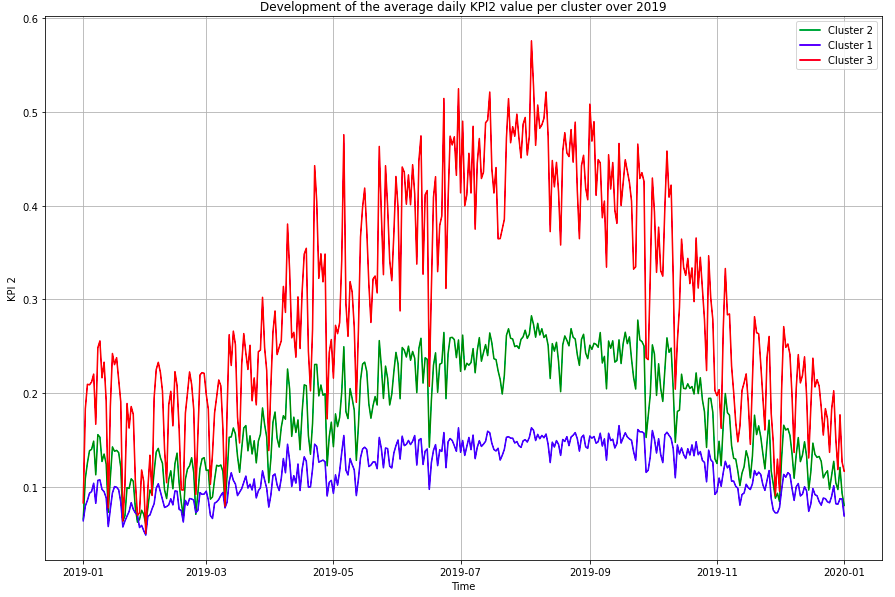
\includegraphics[width=0.7\linewidth]{./Figures/BC_ABB10.png}
    \caption{Development of the average daily KPI2 value per cluster over 2019}
    \label{BCABB10}
\end{figure}

A last insightful clustering using K-Means was created based on the total number of starting rides per station and the average duration of the rides starting there. 4 clusters were found to be suitable (\hyperref[BCABB11]{Appendix Figure X}) and plotting them (\hyperref[BCABB12]{Figure X}) shows, that the red cluster stands out as it exhibits the least proximity to the group of the other three clusters. The yellow and green cluster are relatively similar in terms of their total number of starting rides but seem to show significant differences in terms of the average ride duration starting at the respective stations. When mapping the stations accordingly (\hyperref[BCABB13]{Figure X}), \hyperref[clusterRingsTable]{Table X} summarizes the ring structure.

\begin{figure}[H]
   \centering
    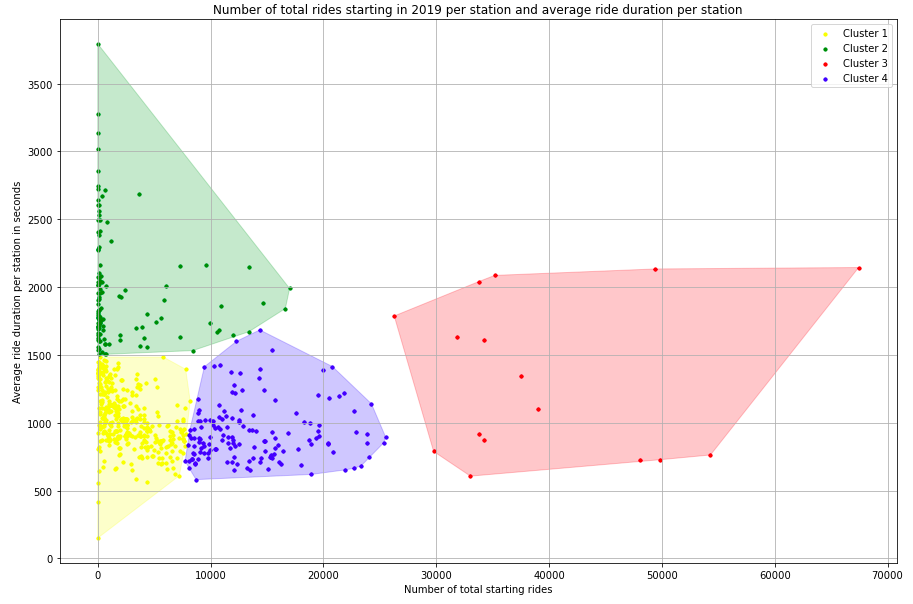
\includegraphics[width=0.8\linewidth]{./Figures/BC_ABB12.png}
    \caption{Number of total rides starting in 2019 per station and average ride duration per station}
    \label{BCABB12}
\end{figure}

\begin{table}[H]
\begin{tabular}{p{0.2\textwidth}p{0.75\textwidth}}
    \toprule
    \textbf{Ring} & \textbf{Description} \\
    \midrule
    Red Cluster & 
    \begin{itemize} 
        \item The red stations are not as predominant as in earlier plots 
        \item They are again mainly located around recreational sites. 
    \end{itemize}\\
    \hline
    Yellow and Green &   \begin{itemize}
        \item The ring comprised by the green and yellow stations exhibits a new structure:
        \item The green stations seem to form a circle around the yellow stations and thus, around the city. 
        \item The green stations seem to form a circle around the yellow stations and thus, around the city. 
        \item Makes sense, as the green stations exhibit roughly the same number of rides as the yellow stations, however they showed a higher average riding duration. 
        \item Thus, the rides from the green outskirt ring seem to be heading towards the center of the city, as their average ride duration is the highest compared to all other clusters
        \item The other clusters do not exhibit this behavior. They might be considered "housing" areas.
    \end{itemize}\\
    \hline
    Blue Cluster & 
    \begin{itemize}
        \item The second ring was also exhibited above
        \item It corresponds to rides roughly as long as the yellow ones
        \item The rides starting there will thus be heading to stations within the blue, red or close yellow stations
    \end{itemize}\\
    \bottomrule
\end{tabular}
\caption{\label{clusterRingsTable}Cluster Rings}
\end{table}


\begin{figure}[H]
   \centering
    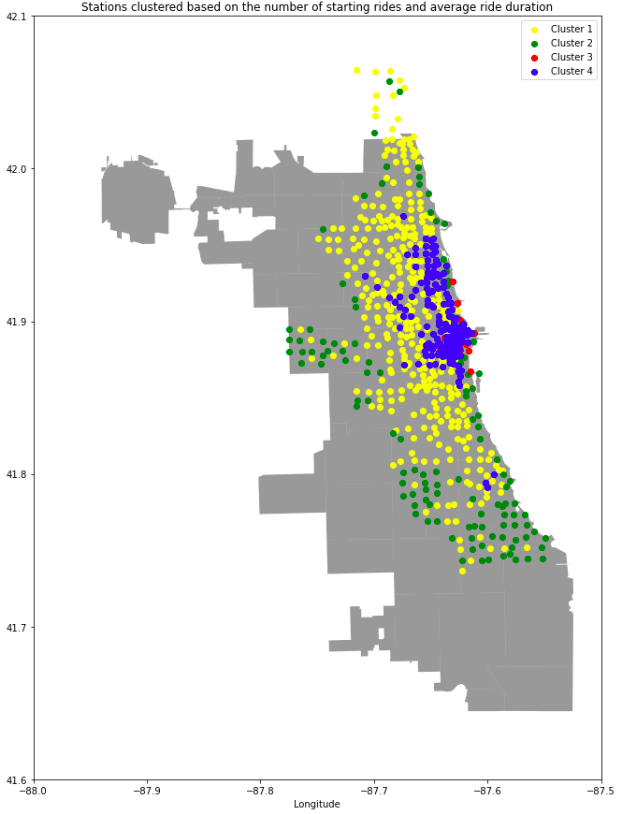
\includegraphics[width=0.8\linewidth]{./Figures/BC_ABB13.png}
    \caption{Stations clustered on the number of starting rides and average ride duration}
    \label{BCABB13}
\end{figure}

\subsection{Predictive Analysis}
\label{subsec:prediction}

As the future demand is a key factor that will guide operational decision-making of Divvy Bikes, total system-level demand in the next hour was forecasted. In order to do that, we developed prediction models with linear regression, random forests and XGBoost. Our features are derived from the dataset \hyperref[Pred_Fig_1]{see Appendix Figure 19}.

We desided to use linear regression models, due to their simplicity and because their use is quasi state-of-the art. While doing so, we immediately faced the problem of missing linearity in our data. Nevertheless, we used Multi-Linear Regression as a first look into regression. Our best model excludes the features ‘season’ and ‘isWeekday’ and reached an r$^{2}$ of roughly 0.6. Because of the missing linearity, we decided to also try Polynomial Regression with the same features, which resulted in strongly improved results. In addition, we also applied both L1 and L2 regularization. In the end, we yield our best Linear/Polynomial Regression model with L1 regularization, with an r$^{2}$ of about 0.9 for the prediction and an MAE around 99.

\begin{figure}[H]
   \centering
    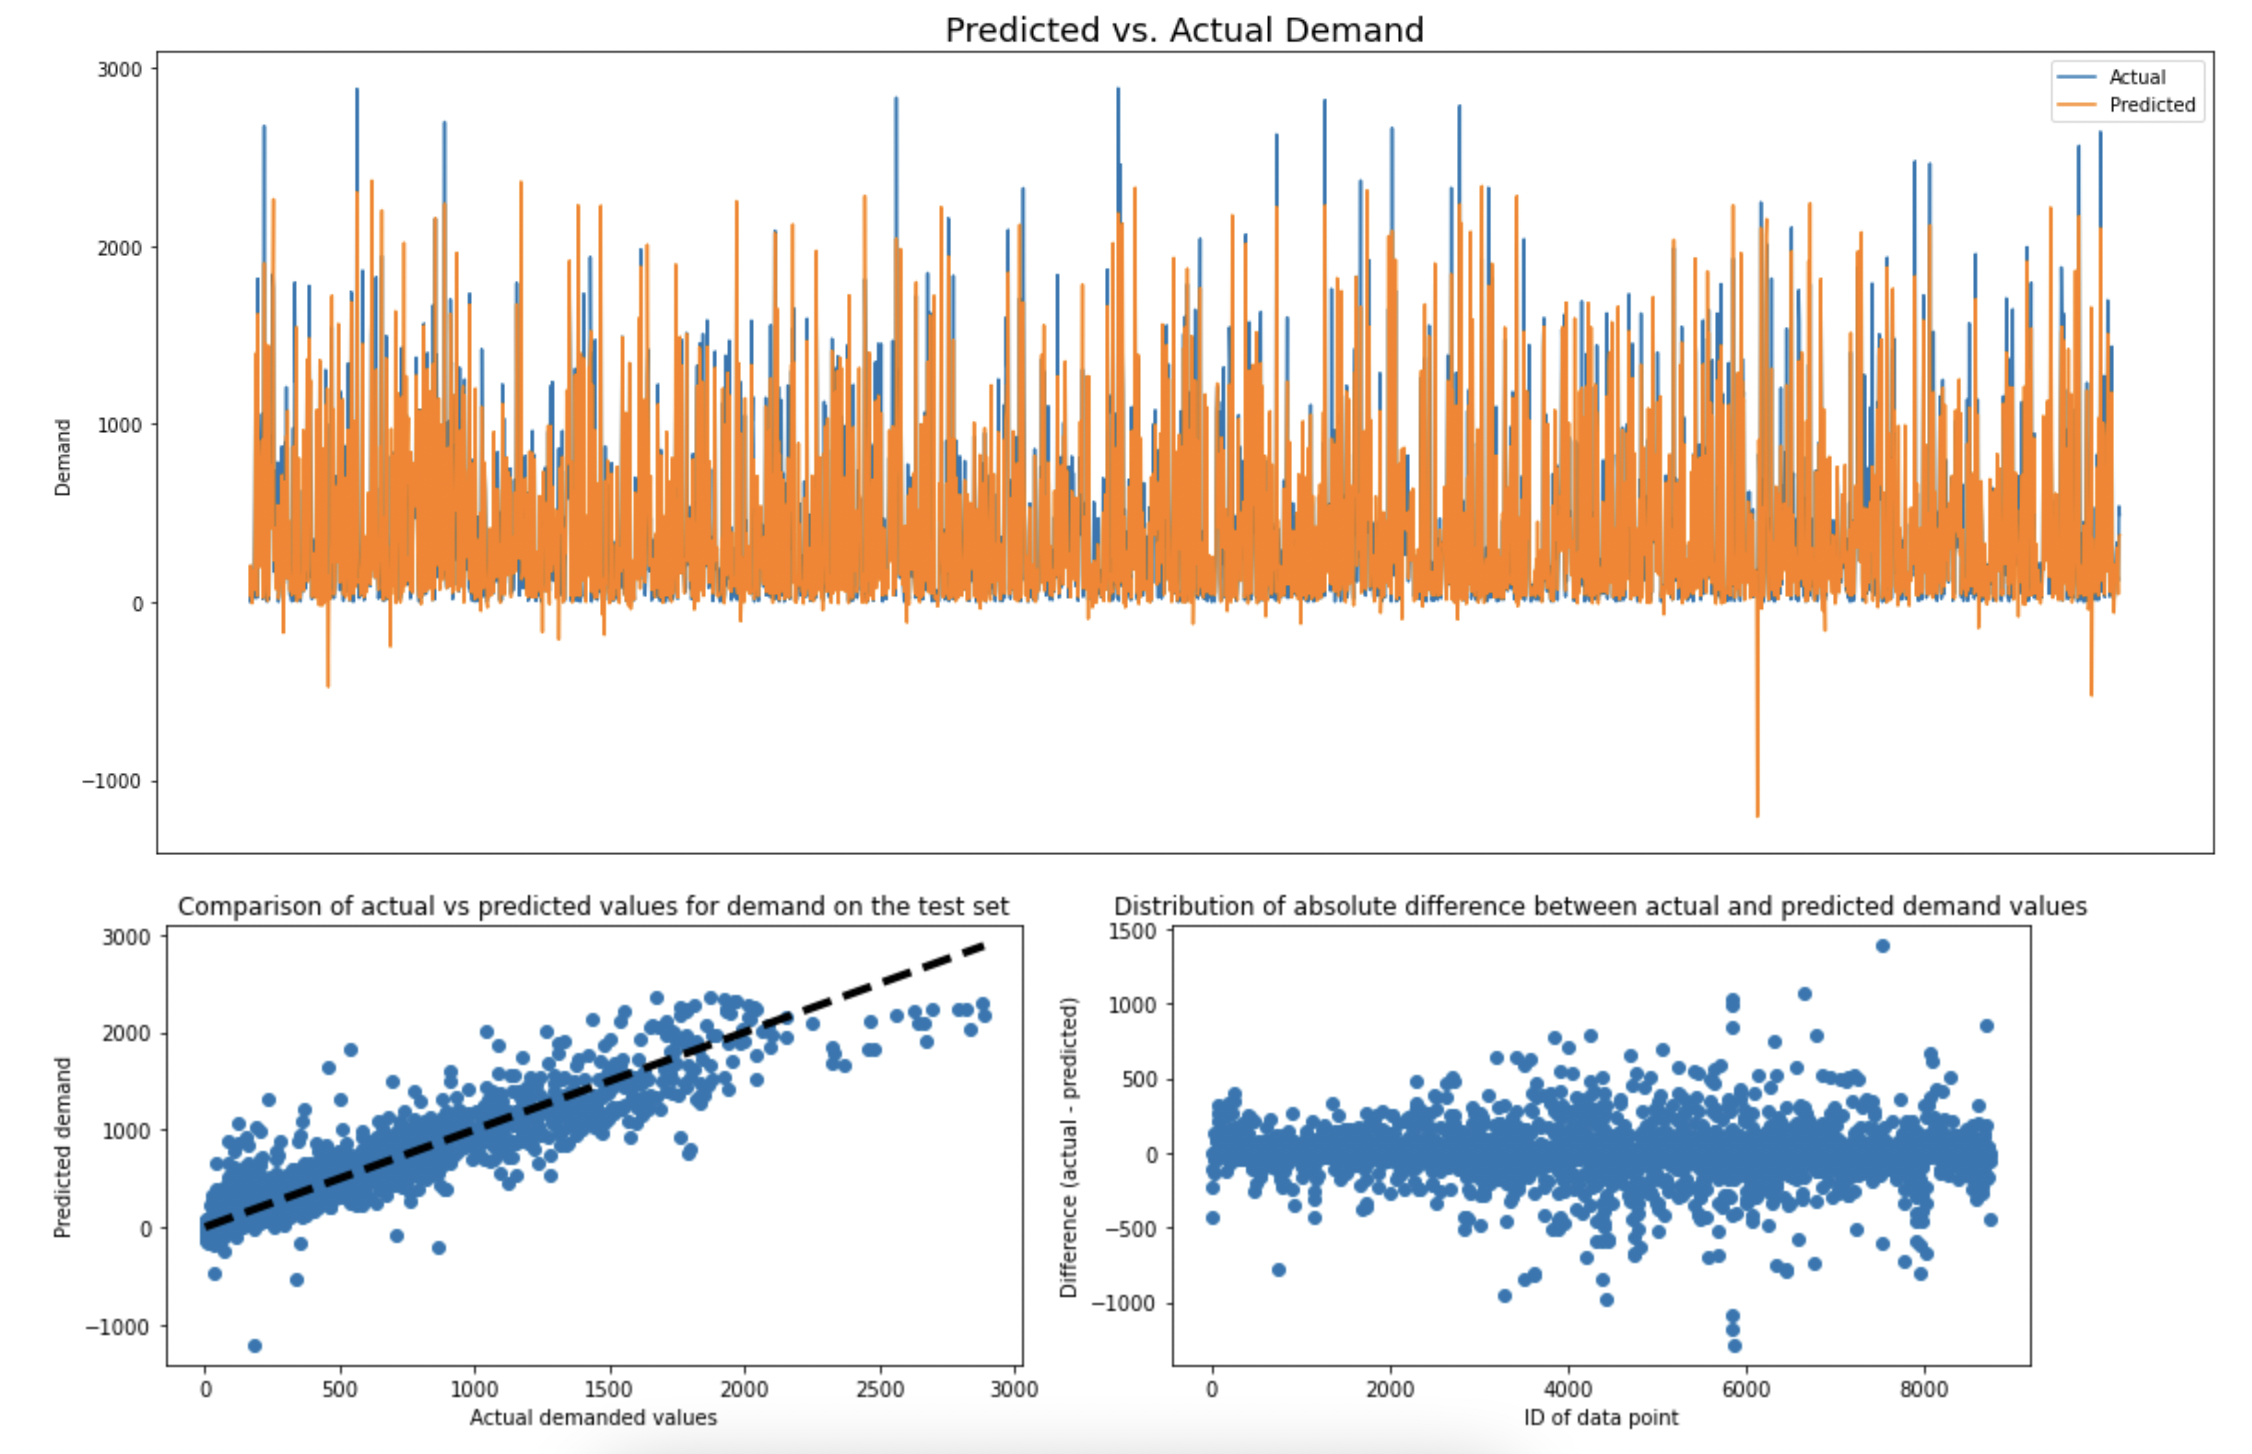
\includegraphics[width=1\linewidth]{./Figures/l1_final.png}
    \caption{Prediction visualization of best L1 model}
    \label{l1}
\end{figure}


For our second and best model, we used the Random Forest algorithm. It is an ensemble method which uses multiple decision trees to make predictions based on a mean computation (in regression) of all trees (see Appendix \hyperref[RF_Intro]{Figure 19} for a visualization). The exact algorithm description and reasons why we chose it as one of our model can be found in the appendix (XXX). To find the best model possible, first a feature selection process was conducted in which different features were selected, and their impact was assessed. Based on their impact on the R2 and MAE and their increase in complexity, the features were then either removed or included in the model. The MAE error metric was used because it has practical relevance, stating that on each hourly prediction x bikes were predicted too much or too less. The R2 error metric describes the proportion of variance in the dependent variable that is accounted for by the model and thus, is also a good measurement of overfitting. The following table illustrates the process. At the end, we decided to select model 5, as model 4 has three more features and is more complex, and the metrics did not differ significantly.
Afterwards, the hyperparameters were tuned and selected. For that, we first looked at the number of estimators (trees in the forest) with cross validation, as can be seen in \hyperref[RF_Fig_1]{Figure 19}. At around 250 estimators, the score does not really change at all, so we picked the number of trees in the forest as 250. To facilitate the hyperparameter tuning and not only focus on one single parameter but on different combinations, we implemented a grid search. Because a whole grid search is computationally heavy, first a random grid search was performed, which limits the possible search space for each optimal parameter. The final results are listed below.
With these values for the hyperparameters, we executed the model on the test set and retrieved an R2 of 91,68 percent.

This means that 91,68 of the proportion of the variance in the demand can be accounted for by the model. The mean absolute error (MAE) is 80,21 which means that in each prediction of the bike demand in one hour, there are 80  too many or too less bikes predicted on average. Benchmarking this, the absolute deviation in the model still seems relatively high, and the Divvy bike provider would still need to maintain 80 additional bikes which are not needed. However, there is a total of more than 6.000 bikes in the Divvy bike fleet, so the prediction error accounts only for about 1 of all bikes which is handleable for the provider. The results of the model are visualized in \hyperref[RF_Fig_2]{Figure 20}. The dashed line would be the optimal prediction line, e.g. if the actual demand is 1.000 the predicted demand would ideally be 1.000 as well. It can be seen that the majority of prediction points reside near the optimal line. In the second figure, the deviations can be inspected more precise. Most of the prediction points lie between -100 and 100 which is as also expressed through the mean absolute error (MAE) of 80. However, some outliers to exist with the extreme of approximately -1.500 demanded bikes on one day.
\begin{figure}[H]
   \centering
    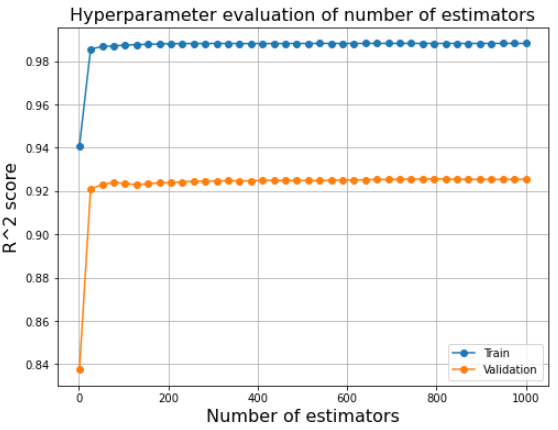
\includegraphics[width=0.5\linewidth]{./Figures/RF_Fig_2.png}
    \caption{Hyperpararmeter evaluation of number of estimators}
    \label{RF_Fig_2}
\end{figure}

\begin{figure}[H]
   \centering
    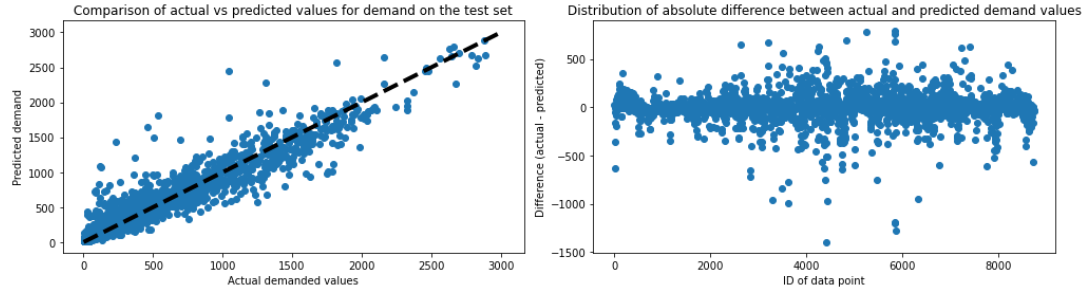
\includegraphics[width=1\linewidth]{./Figures/RF_Fig_3.png}
    \caption{Comparison of actual vs predicted values for demand on the test set and Distribution of absolute difference between actual and predected demand values}
    \label{RF_Fig_3}
\end{figure}
As third regression algorithm we decided to use XGBoost, an ensemble method. The "state-of-the-art” machine learning algorithm can deal well with structured data and is fast, especially compared to other implementations of gradient boosting. The results of the first model are good with a R-squared error of 97 for the train and 92 for validation. Also, the mean absolute error (MAE) and the Root Mean Squared Error (RMSE) indicate that the model is relatively accurate. Using grid search to tune the hyperparameters improved the model, but only slightly resulting in a R-squared error of 93 for the validation.
\begin{figure}[H]
   \centering
    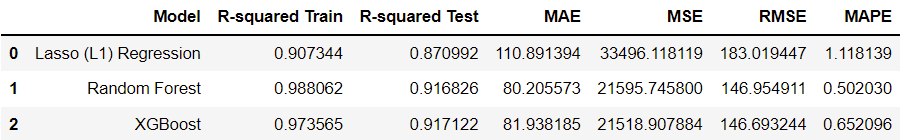
\includegraphics[width=1\linewidth]{./Figures/Predictive_Table_Result.png}
    \caption{Predective analytics results}
    \label{RF_Fig_4}
\end{figure}


\section{Conclusion}
\label{sec:Conclusion}

In conclusion, the project delivers valuable insights into the bike fleet’s performance and an hourly demand prediction.

Averaging over all yearly bikes, the fleet does not meet the target number of rides of 4-6 defined by Boor (2019), so there might be too many bikes or improperly distributed bikes, especially during winter.  The vast majority of stations are properly equipped in terms of capacity. “Outskirt" capacity might even be too high, thus it could be considered to relocate some bikes towards the center. 

A three ring structure could be exhibited, with the red, most centered ring being that with the highest demand and activity. The red stations are predominantly  in recreational sites. Combining this insight with the fact that the duration of rides in summer is significantly longer, we can conclude that leisure rides during summer and commuters seem to be the most important customer groups. Those groups could be advertised specifically.

In terms of revenue, there are different possibilities to change the pricing in order to increase the profitability. First, looking at the “three-ring-structure”, different pricing for the rings could be adapted. Furthermore, the bike rentals in winter should be made more attractive and thus the pricing in winter could be adjusted. Another idea is to introduce a different pricing structure for the extra minutes. During the day the longest duration is between 10am and 5pm and the second longest is during 12pm and 4 am, hence the trips could be more expensive per minute in these time intervals.

However, there are some limitations to our project. The demand is predicted for the whole system, but predicting the demand on single stations is more accurate and enables better maintenance and refilling of bikes. Moreover, time series analysis over multiple years could be used to improve prediction. Also, we were limited by the given data and collecting more detailed data offers new options for further analysis.



%%%%%%%%%%%%%%%%%%%%%%%%%%%%%%%%%%%%%%%%%%%%%%%%%%%%%%%%%%%%%
%APPENDICES
%%%%%%%%%%%%%%%%%%%%%%%%%%%%%%%%%%%%%%%%%%%%%%%%%%%%%%%%%%%%%


\appendix
\renewcommand*{\thesection}{\Alph{section}}\textbf{}

% APPENDIX A
\clearpage
\section{Appendix}
\label{app:A}

\subsection{Data Description}
\label{app:A1}

\begin{table}[H]
\centering
\begin{tabular}{p{0.2\textwidth}p{0.75\textwidth}}
\toprule
Data inputs & Description \\
\midrule
start\_time
& 
Time where trips are started : datetime  \\

end\_time
&
Time where trips are finished : datetime \\

start\_station\_id
&
ID for start station : integer   \\

start\_station\_name 
&
Name for start station : string \\

end\_station\_name 
&
Name for end station : string \\

bike\_id 
&
ID for unique bike : integer \\

user\_type 
&
Subscriber and customer are distinguished : string \\

duration\_time 
&
Duration of trip (in sec., min., hour) : integer \\

weekday\_start 
&
Indicating weekday (true/false) : boolean \\

full\_hour\_start 
&
Start time rounded to full hour : datetime \\

max\_temp 
&
Describing temperature values in Celsius : float \\

precip 
&
Indicating rain/snow (true/false) : boolean \\

total\_docks 
&
Theoretical maximum capacity of the station : integer \\

docks\_in\_service 
&
Actual capacity of the station : integer \\

status 
&
Availability of the stations : string \\

start\_latitude 
&
Latitude of the starting station : float \\

start\_longitude 
&
Longitude of the start station : float \\






\bottomrule
\end{tabular}
\caption[Data description of most relevant data inputs]{Data description of most relevant data inputs}
\label{tab:dataDescription}
\end{table} \\


\subsection{Temporal Demand Patterns and Seasonality}
\label{app:A2}

\begin{figure}[H]
    \centering
    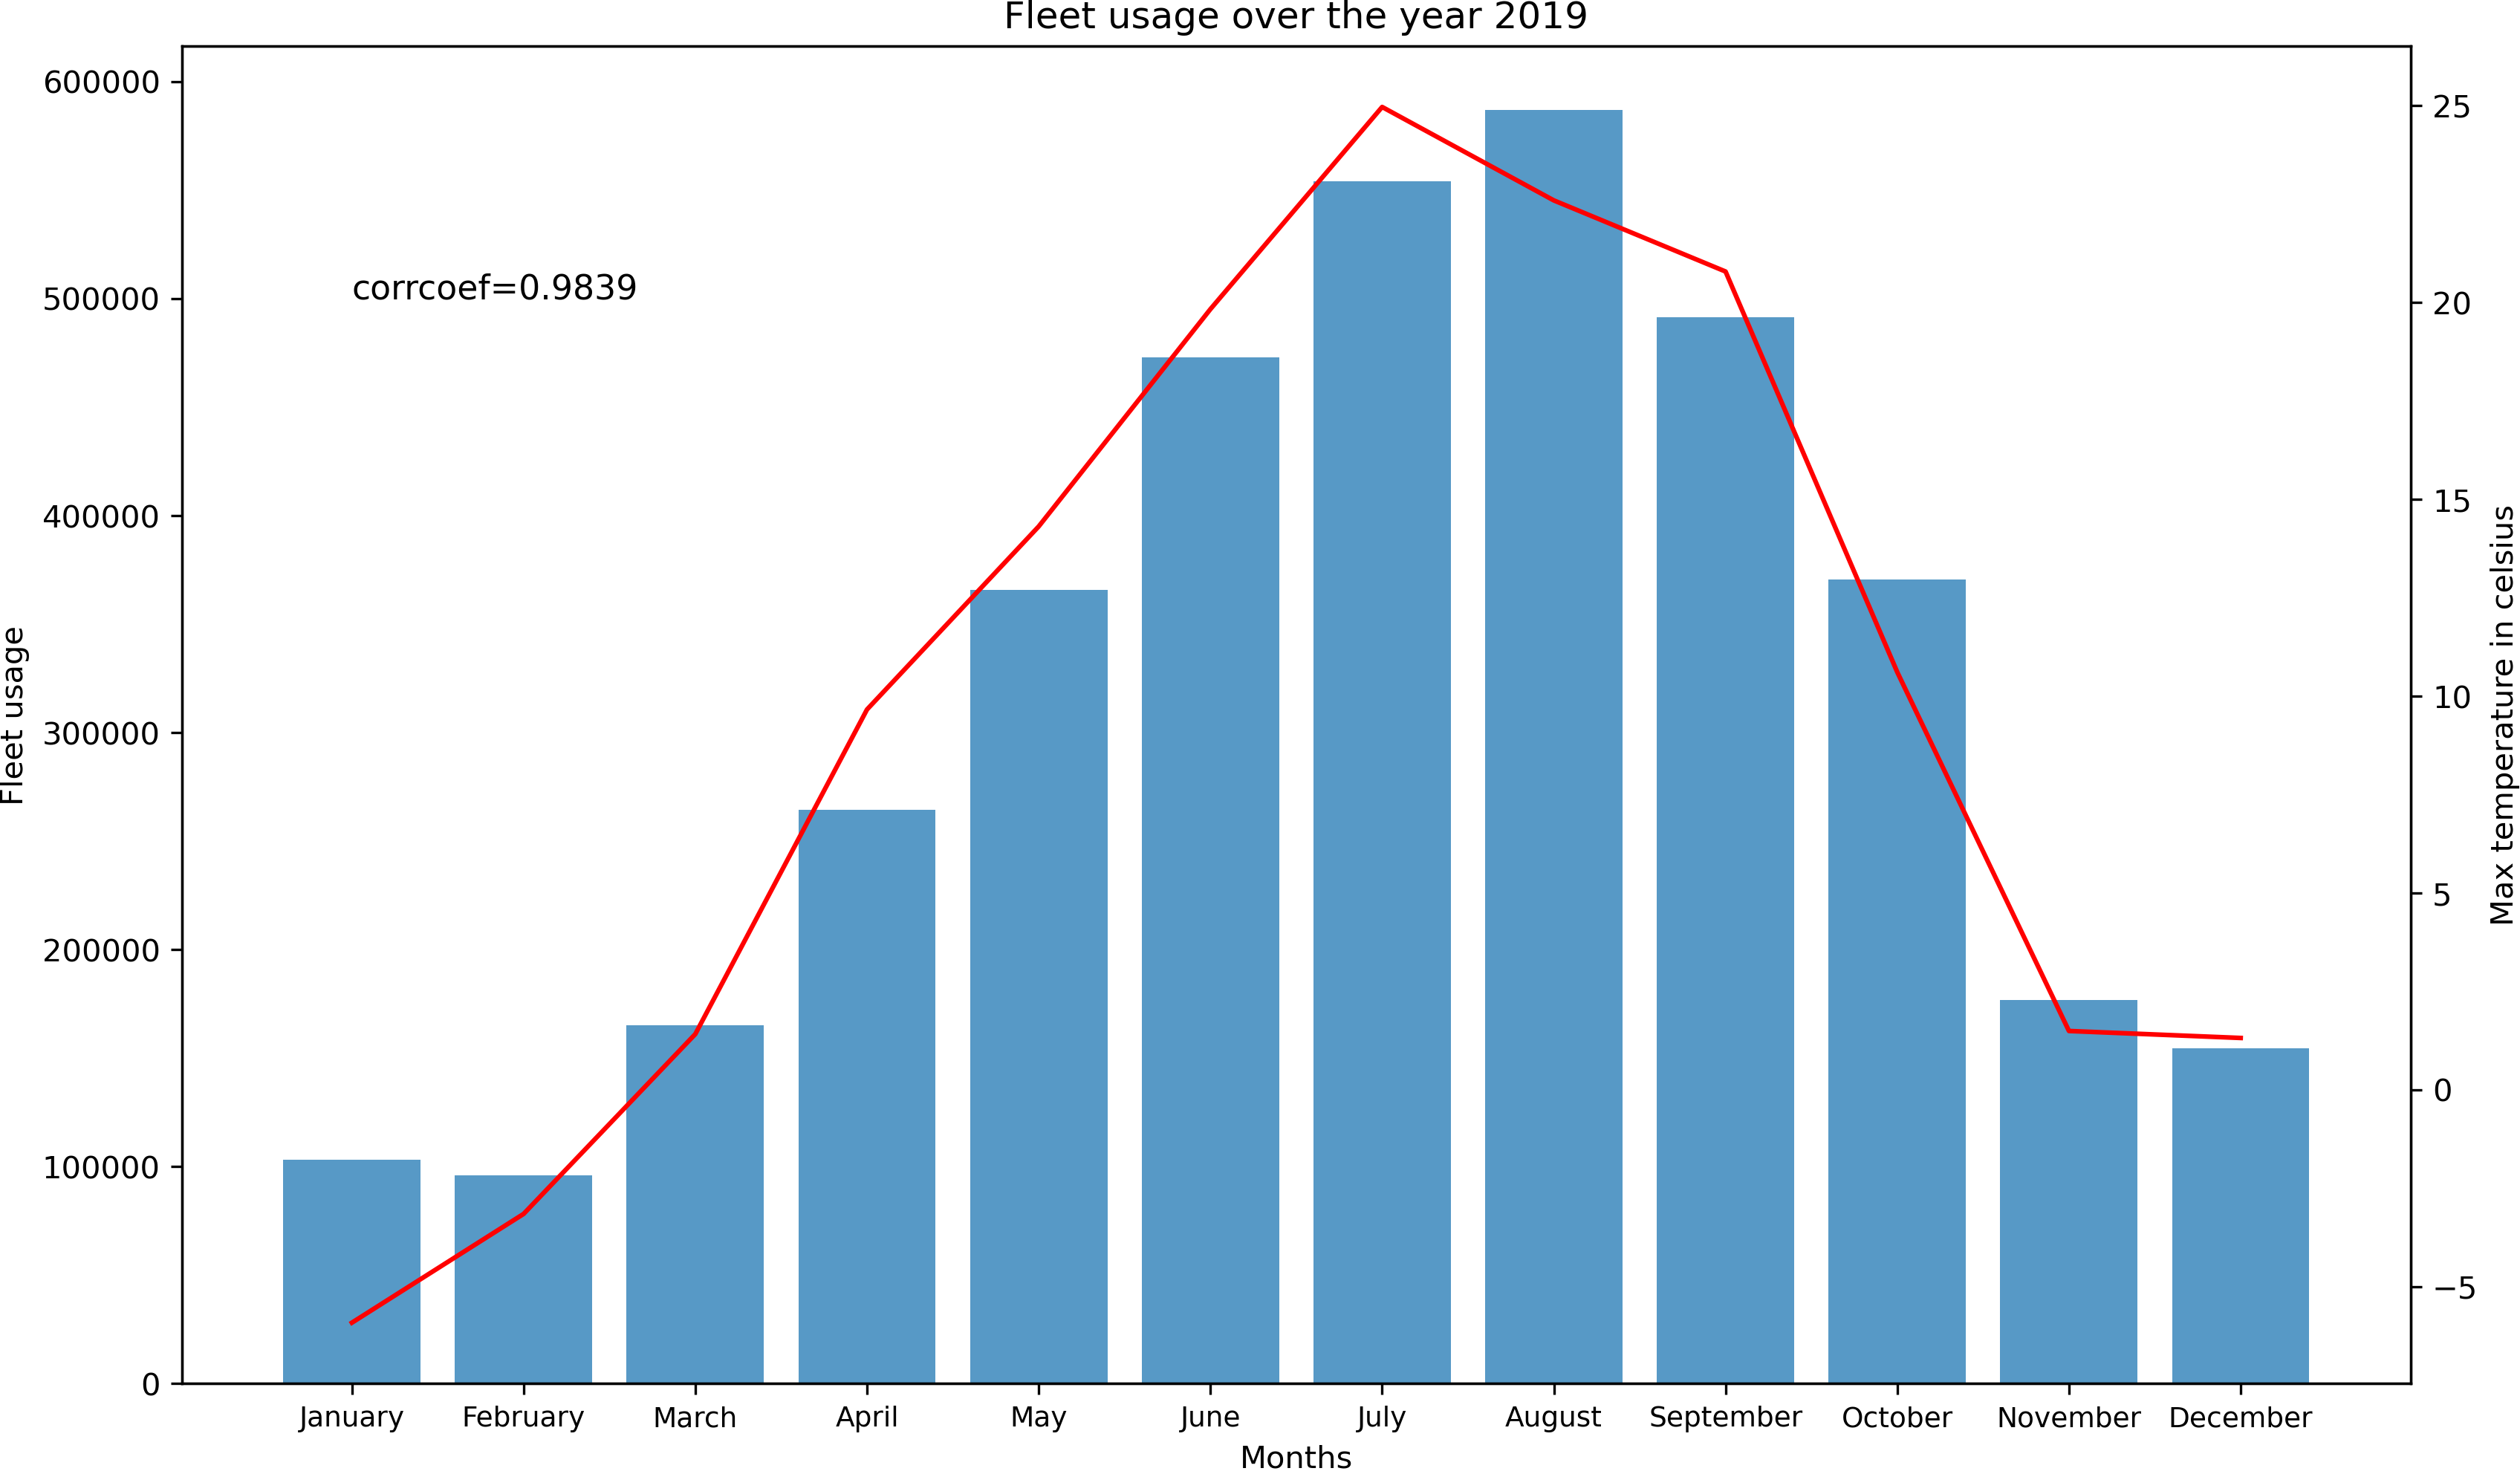
\includegraphics[width=1\linewidth]{./Figures/fleetUsageYear.png}
    \caption{Fleet usage over the year 2019}
    \label{fleetUsageYear}
\end{figure}

\begin{figure}[H]
    \centering
    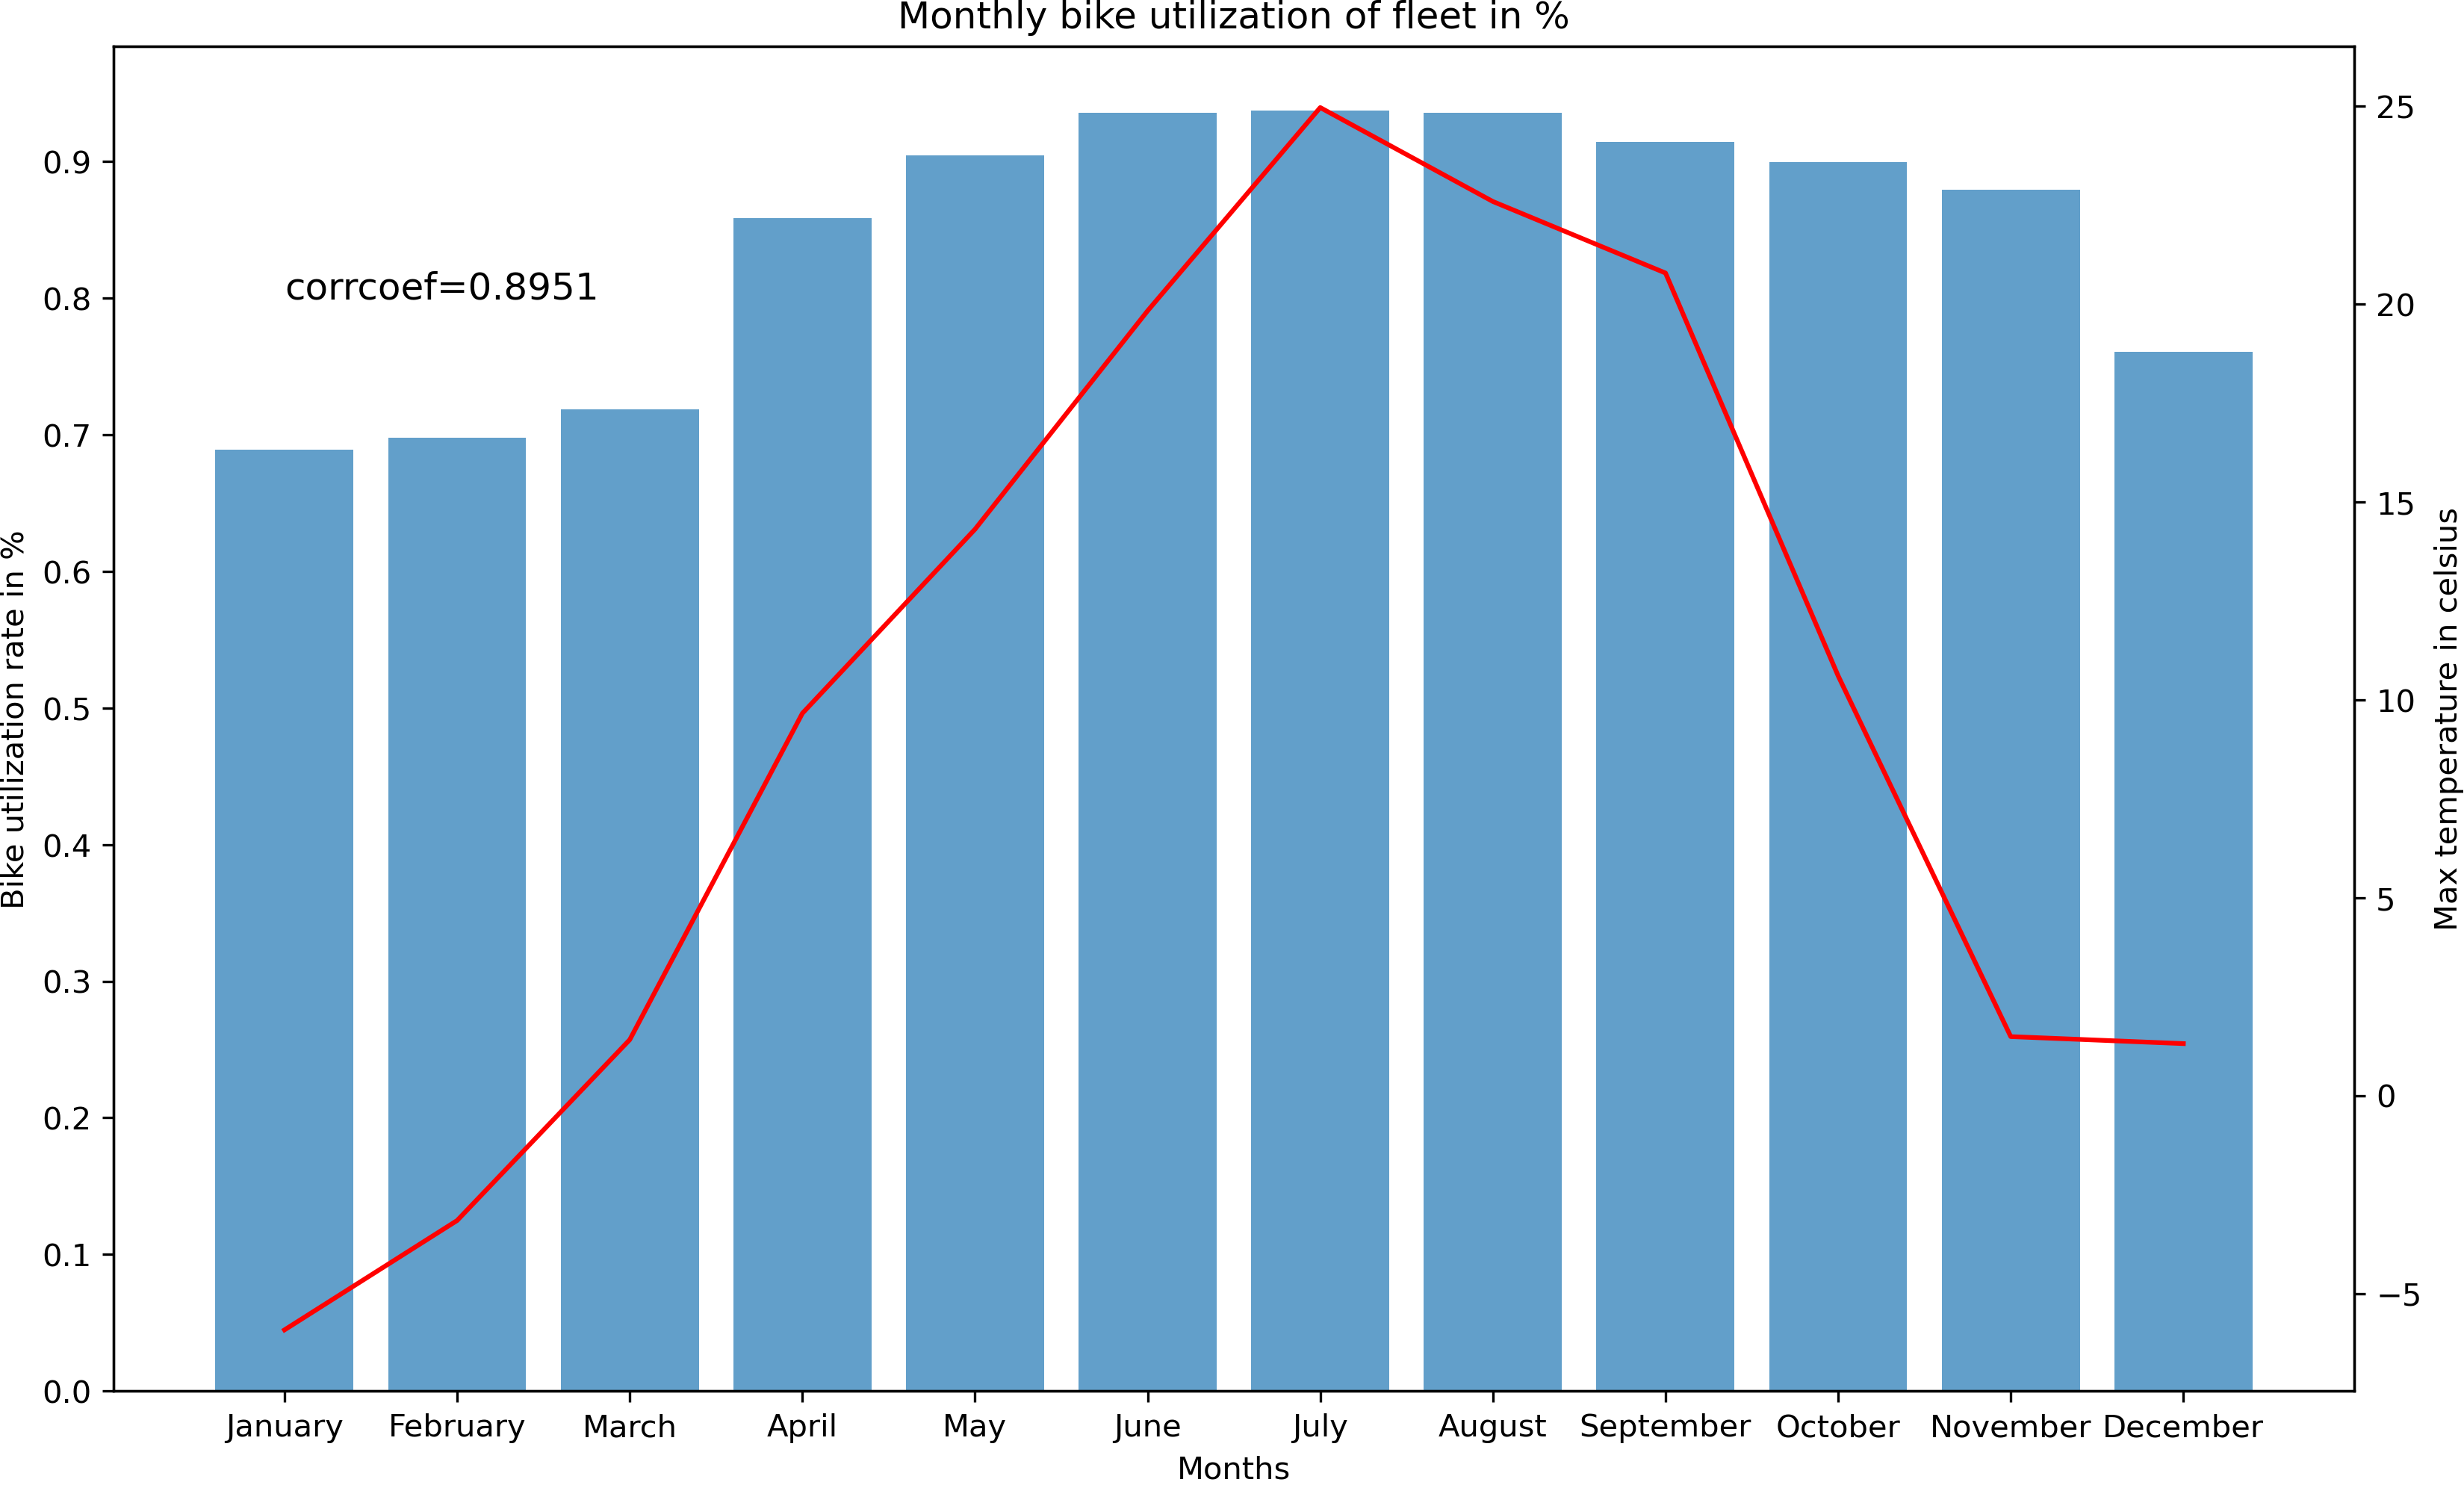
\includegraphics[width=1\linewidth]{./Figures/fleetUtilizationYear.png}
    \caption{Bike utilization over the year 2019}
    \label{fleetUtilizationYear}
\end{figure}

\begin{figure}[H]
   \centering
    \includegraphics[width=0.8\linewidth]{./Figures/DailyUsageWithPrecip.png}
    \caption{Daily bike usage of fleet with precip for each month}
    \label{DailyUsageWithPrecip}
\end{figure}

\begin{figure}[H]
   \centering
    \includegraphics[width=0.8\linewidth]{./Figures/DailyUtilizationWithPrecip.png}
    \caption{Daily bike utilization of fleet with precip for each month}
    \label{DailyUtilizationWithPrecip}
\end{figure}

\subsection{KPI 1: RPUB (Rides Per Unique Bike)}
\label{app:A3}

\subsection*{Weather-based investigation of RPUB}
\label{app:A1}

To be able to also take into account some of the weather data, two metrics were developed. Firstly, if more than half of all rides on one day started during rain, then the day was counted as "rainday". Secondly, if the average temperature was above ten degrees, the day was counted as "warmday".
In the first boxplot, the data (RPUB with unique yearly bikes) is split in terms of weath-er the day was rainy and weather it was warm. It becomes clear that the variance of the RPUB on a rainday is significantly smaller than on a non-rainy day. This might be due to the fact that regardless of the temperature or other aspects that might influence usage, people will refrain from using the bike, leading to less fluctuation in terms of the RPUB. As to expect, the RPUB is much higher on warm days. 

\begin{figure}[H]
   \centering
    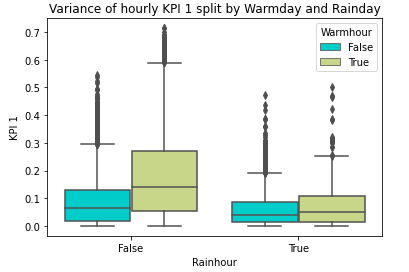
\includegraphics[width=0.8\linewidth]{./Figures/APP1.png}
    \caption{Variance of hourly RPUB split by Warmday and Rainday}
    \label{APP1}
\end{figure}

\begin{figure}[H]
   \centering
    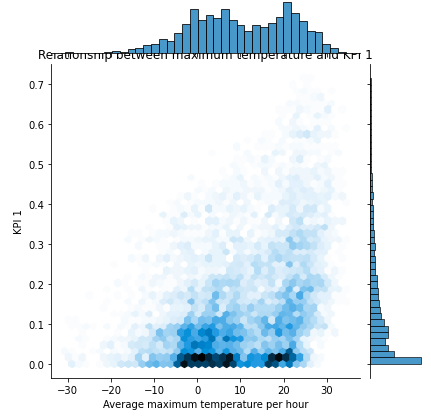
\includegraphics[width=0.8\linewidth]{./Figures/APP2.png}
    \caption{Relationship between maximum temperature and RPUB}
    \label{APP2}
\end{figure}

Investigating a jointplot illustrating the relationship between maximum temperature and RPUB with unique yearly bikes, a linear positive correlation between the average maxi-mum daily temperature and the RPUB (thus, bike usage) can be exhibited. However, the his-togram of RPUB values is comparably equally distributed, being slightly skewed towards low values.

\subsection{KPI 2: Demand-Capacity}
\label{app:A4}

\begin{figure}[H]
   \centering
    \includegraphics[width=0.8\linewidth]{./Figures/kpi2abb2.png}
    \caption{Average hourly KPI 2 value grouped by month}
    \label{kpi2abb2}
\end{figure}

\begin{figure}[H]
   \centering
    \includegraphics[width=0.8\linewidth]{./Figures/kpi2abb3.png}
    \caption{Average hourly KPI 2}
    \label{kpi2abb3}
\end{figure}

\subsection*{More thorough investigation of Demand-Capacity}
\label{app:A2}

\begin{figure}[H]
   \centering
    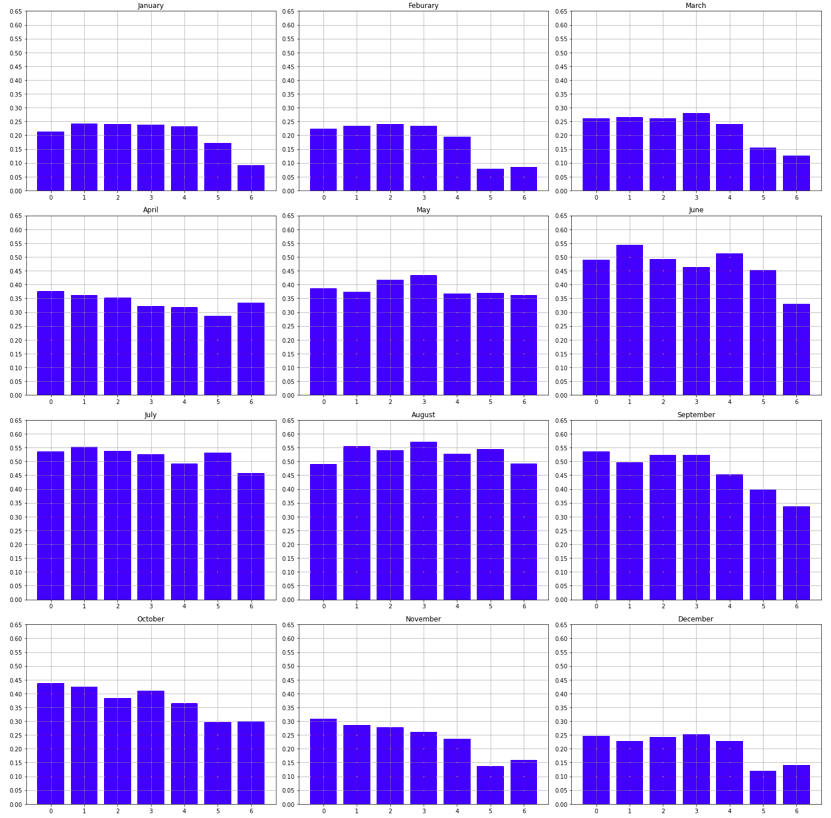
\includegraphics[width=0.8\linewidth]{./Figures/APP1_1.png}
    \caption{Average Demand-Capacity per day per month}
    \label{APP1-1}
\end{figure}

The illustration above depicts the avergage demand-capacity value per day per month. This stresses the notion that was already gained in the main part of this assignment in a sense, that the figures do not, on average, come close to a problematic value of 1.


\subsection{KPI 3: Average Rental Durations}
\label{app:A5}

\begin{figure}[H]
   \centering
    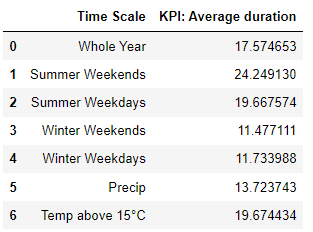
\includegraphics[width=0.4\linewidth]{./Figures/Duration_Fig_2.png}
    \caption{Results KPI 3 Average Rental Durations}
    \label{Duration_Fig_2}
\end{figure}

\subsection{KPI 4: Revenue}
\label{app:A6}

\begin{figure}[H]
    \centering
    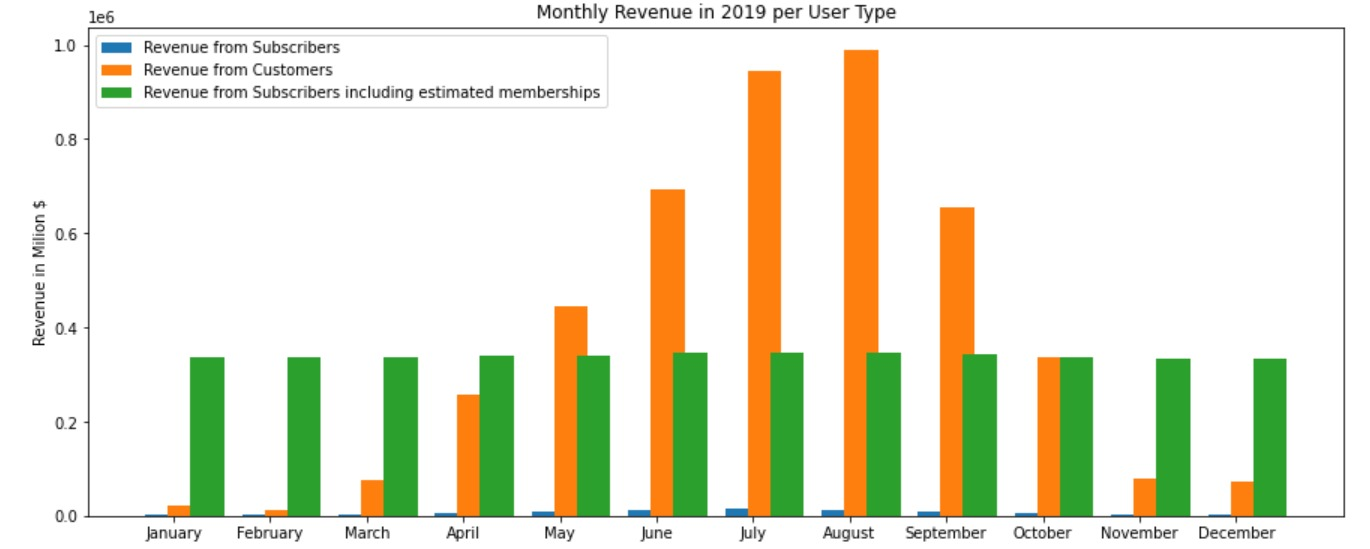
\includegraphics[width=0.9\linewidth]{./Figures/Revenue_monthlyUserType.jpeg}
    \caption{Monthly Revenue in 2019 per User Type}
    \label{fig_revenue_2}
\end{figure}

\begin{figure}[H]
    \centering
    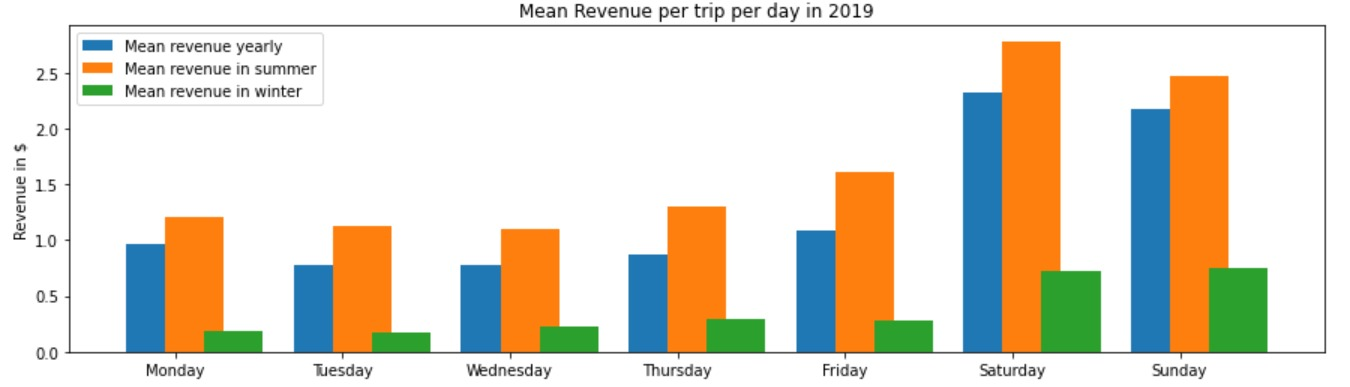
\includegraphics[width=0.9\linewidth]{./Figures/Revenue_week.jpeg}
    \caption{Mean Revenue per trip per day in 2019}
    \label{fig_revenue_3}
\end{figure}

\subsection{Cluster Analysis}
\label{app:A7}

\begin{figure}[H]
   \centering
    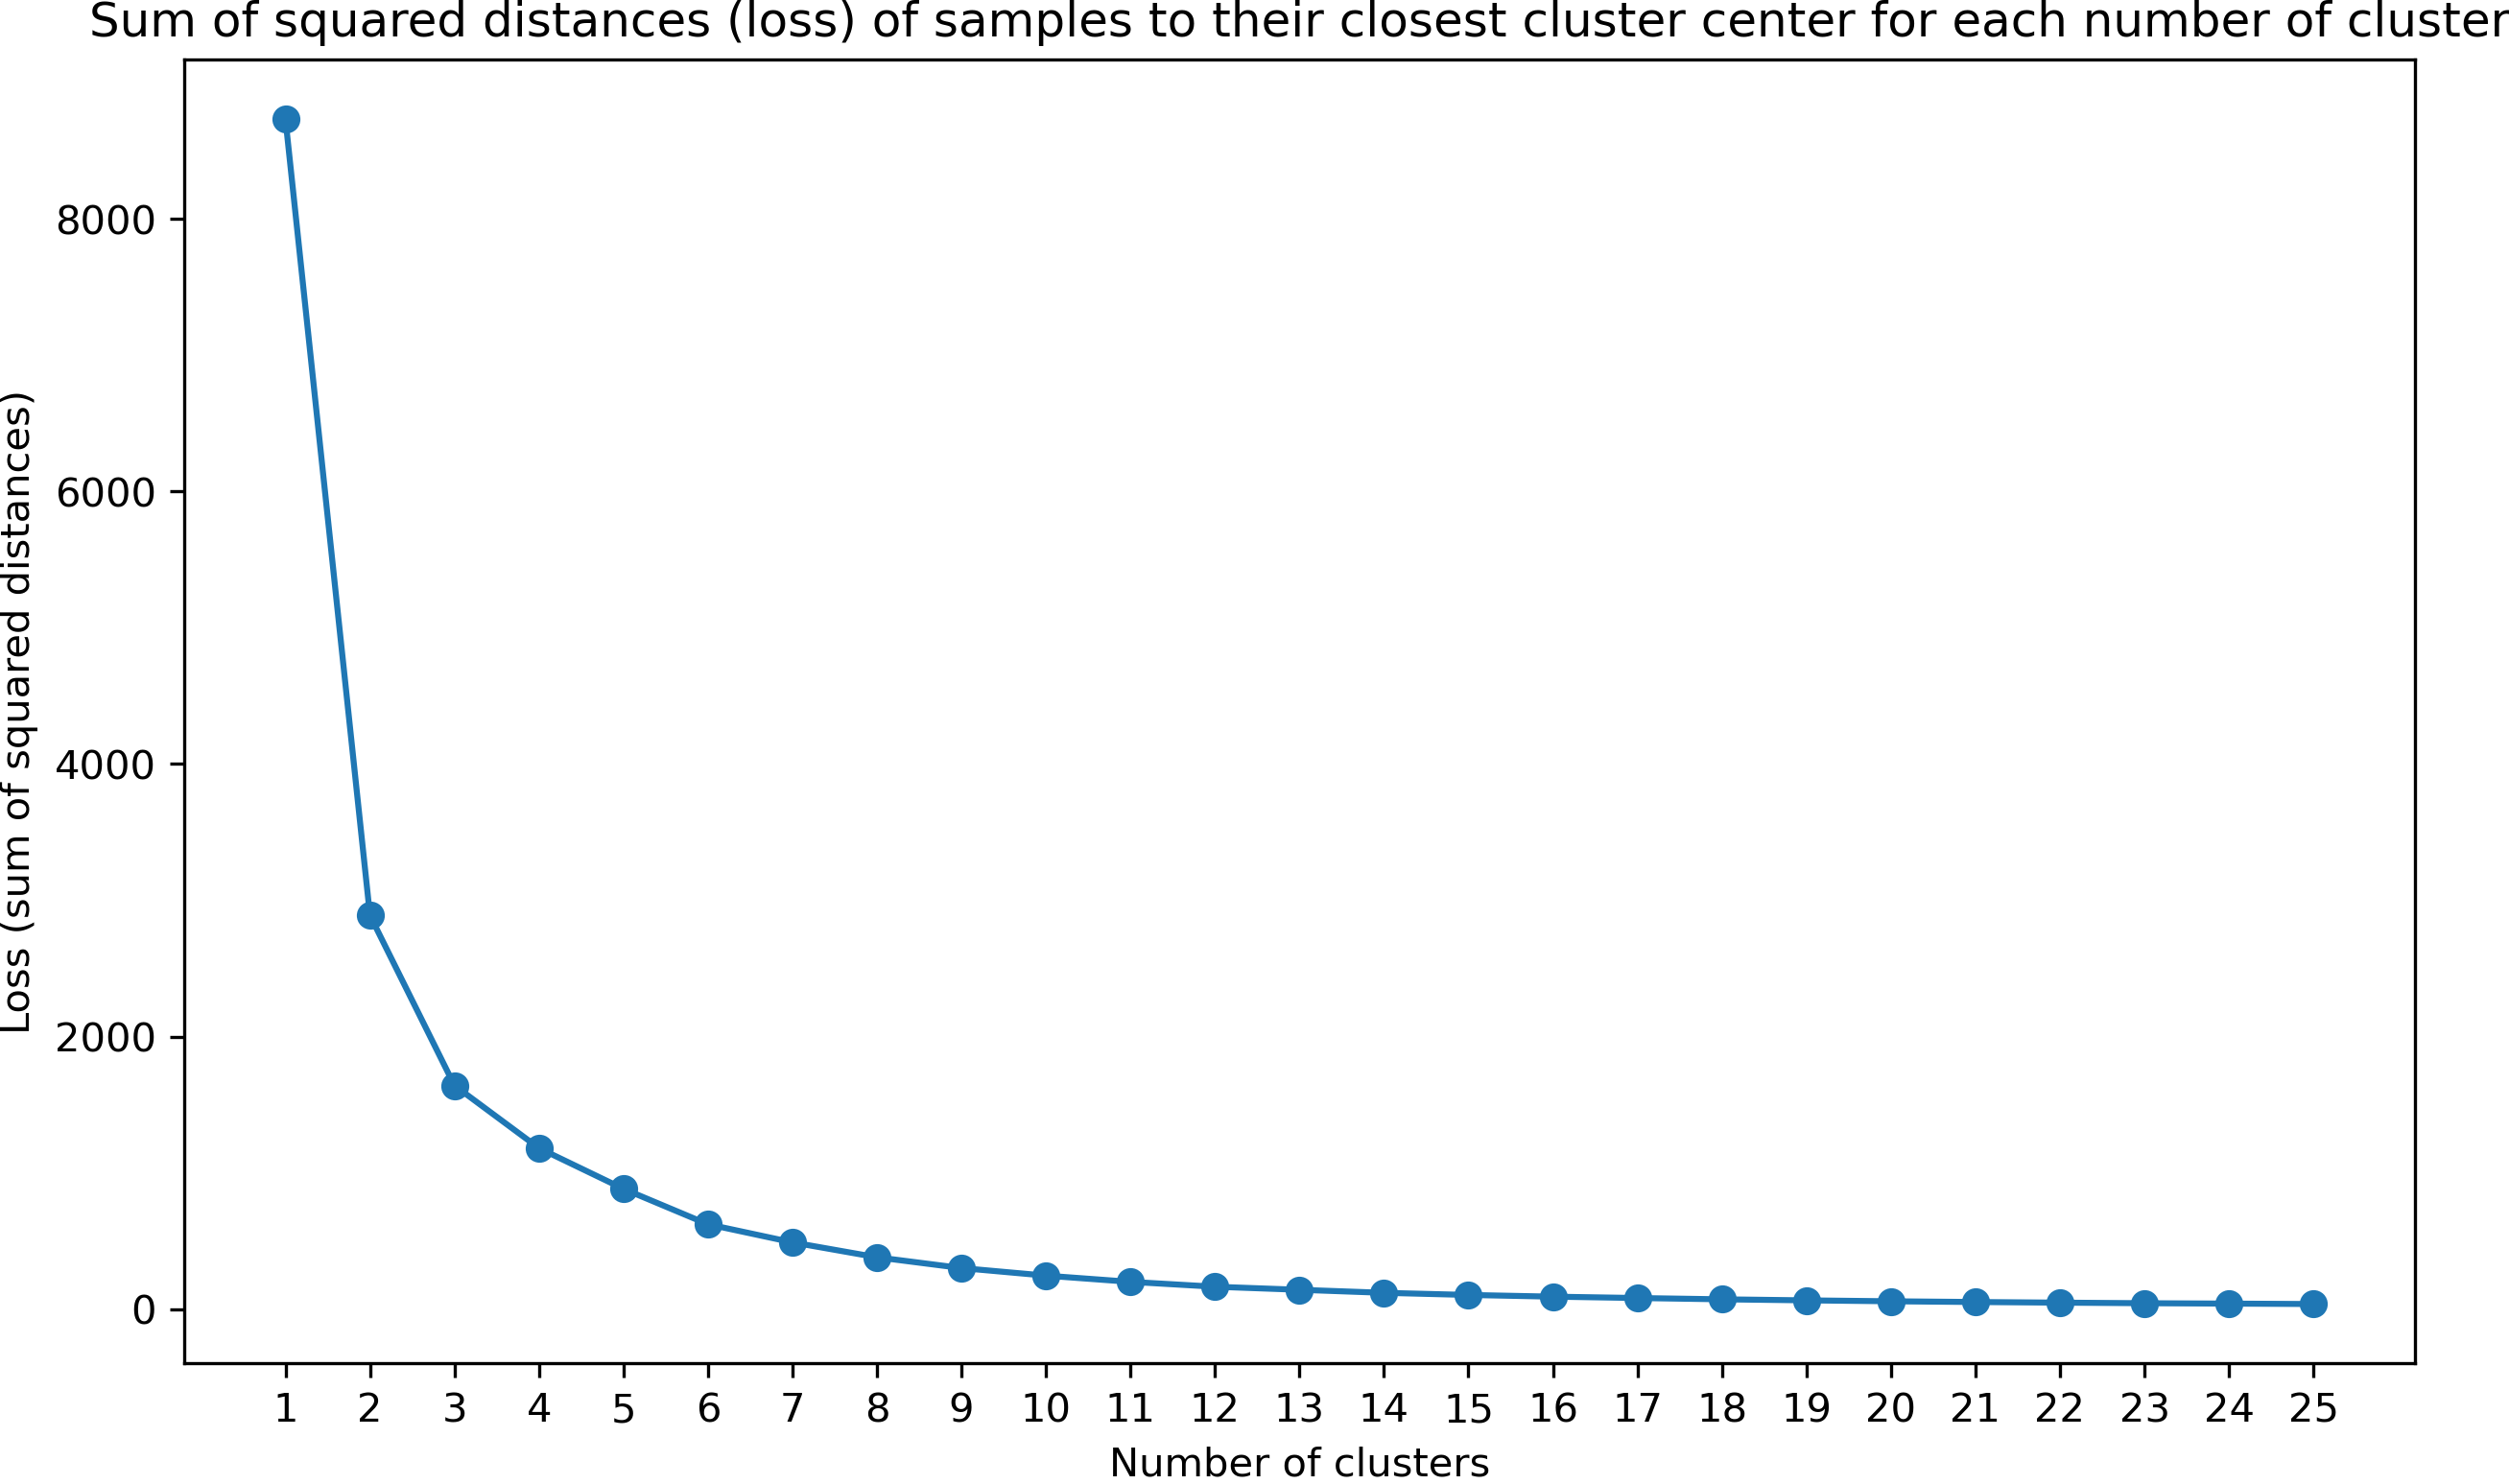
\includegraphics[width=0.8\linewidth]{./Figures/LossKMeans_Duration_dpi300.png}
    \caption{Sum of squared distances (loss) of samples to their closest cluster center for each number of cluster for duration}
    \label{LossKMeans_Duration_dpi300}
\end{figure}

\begin{figure}[H]
   \centering
    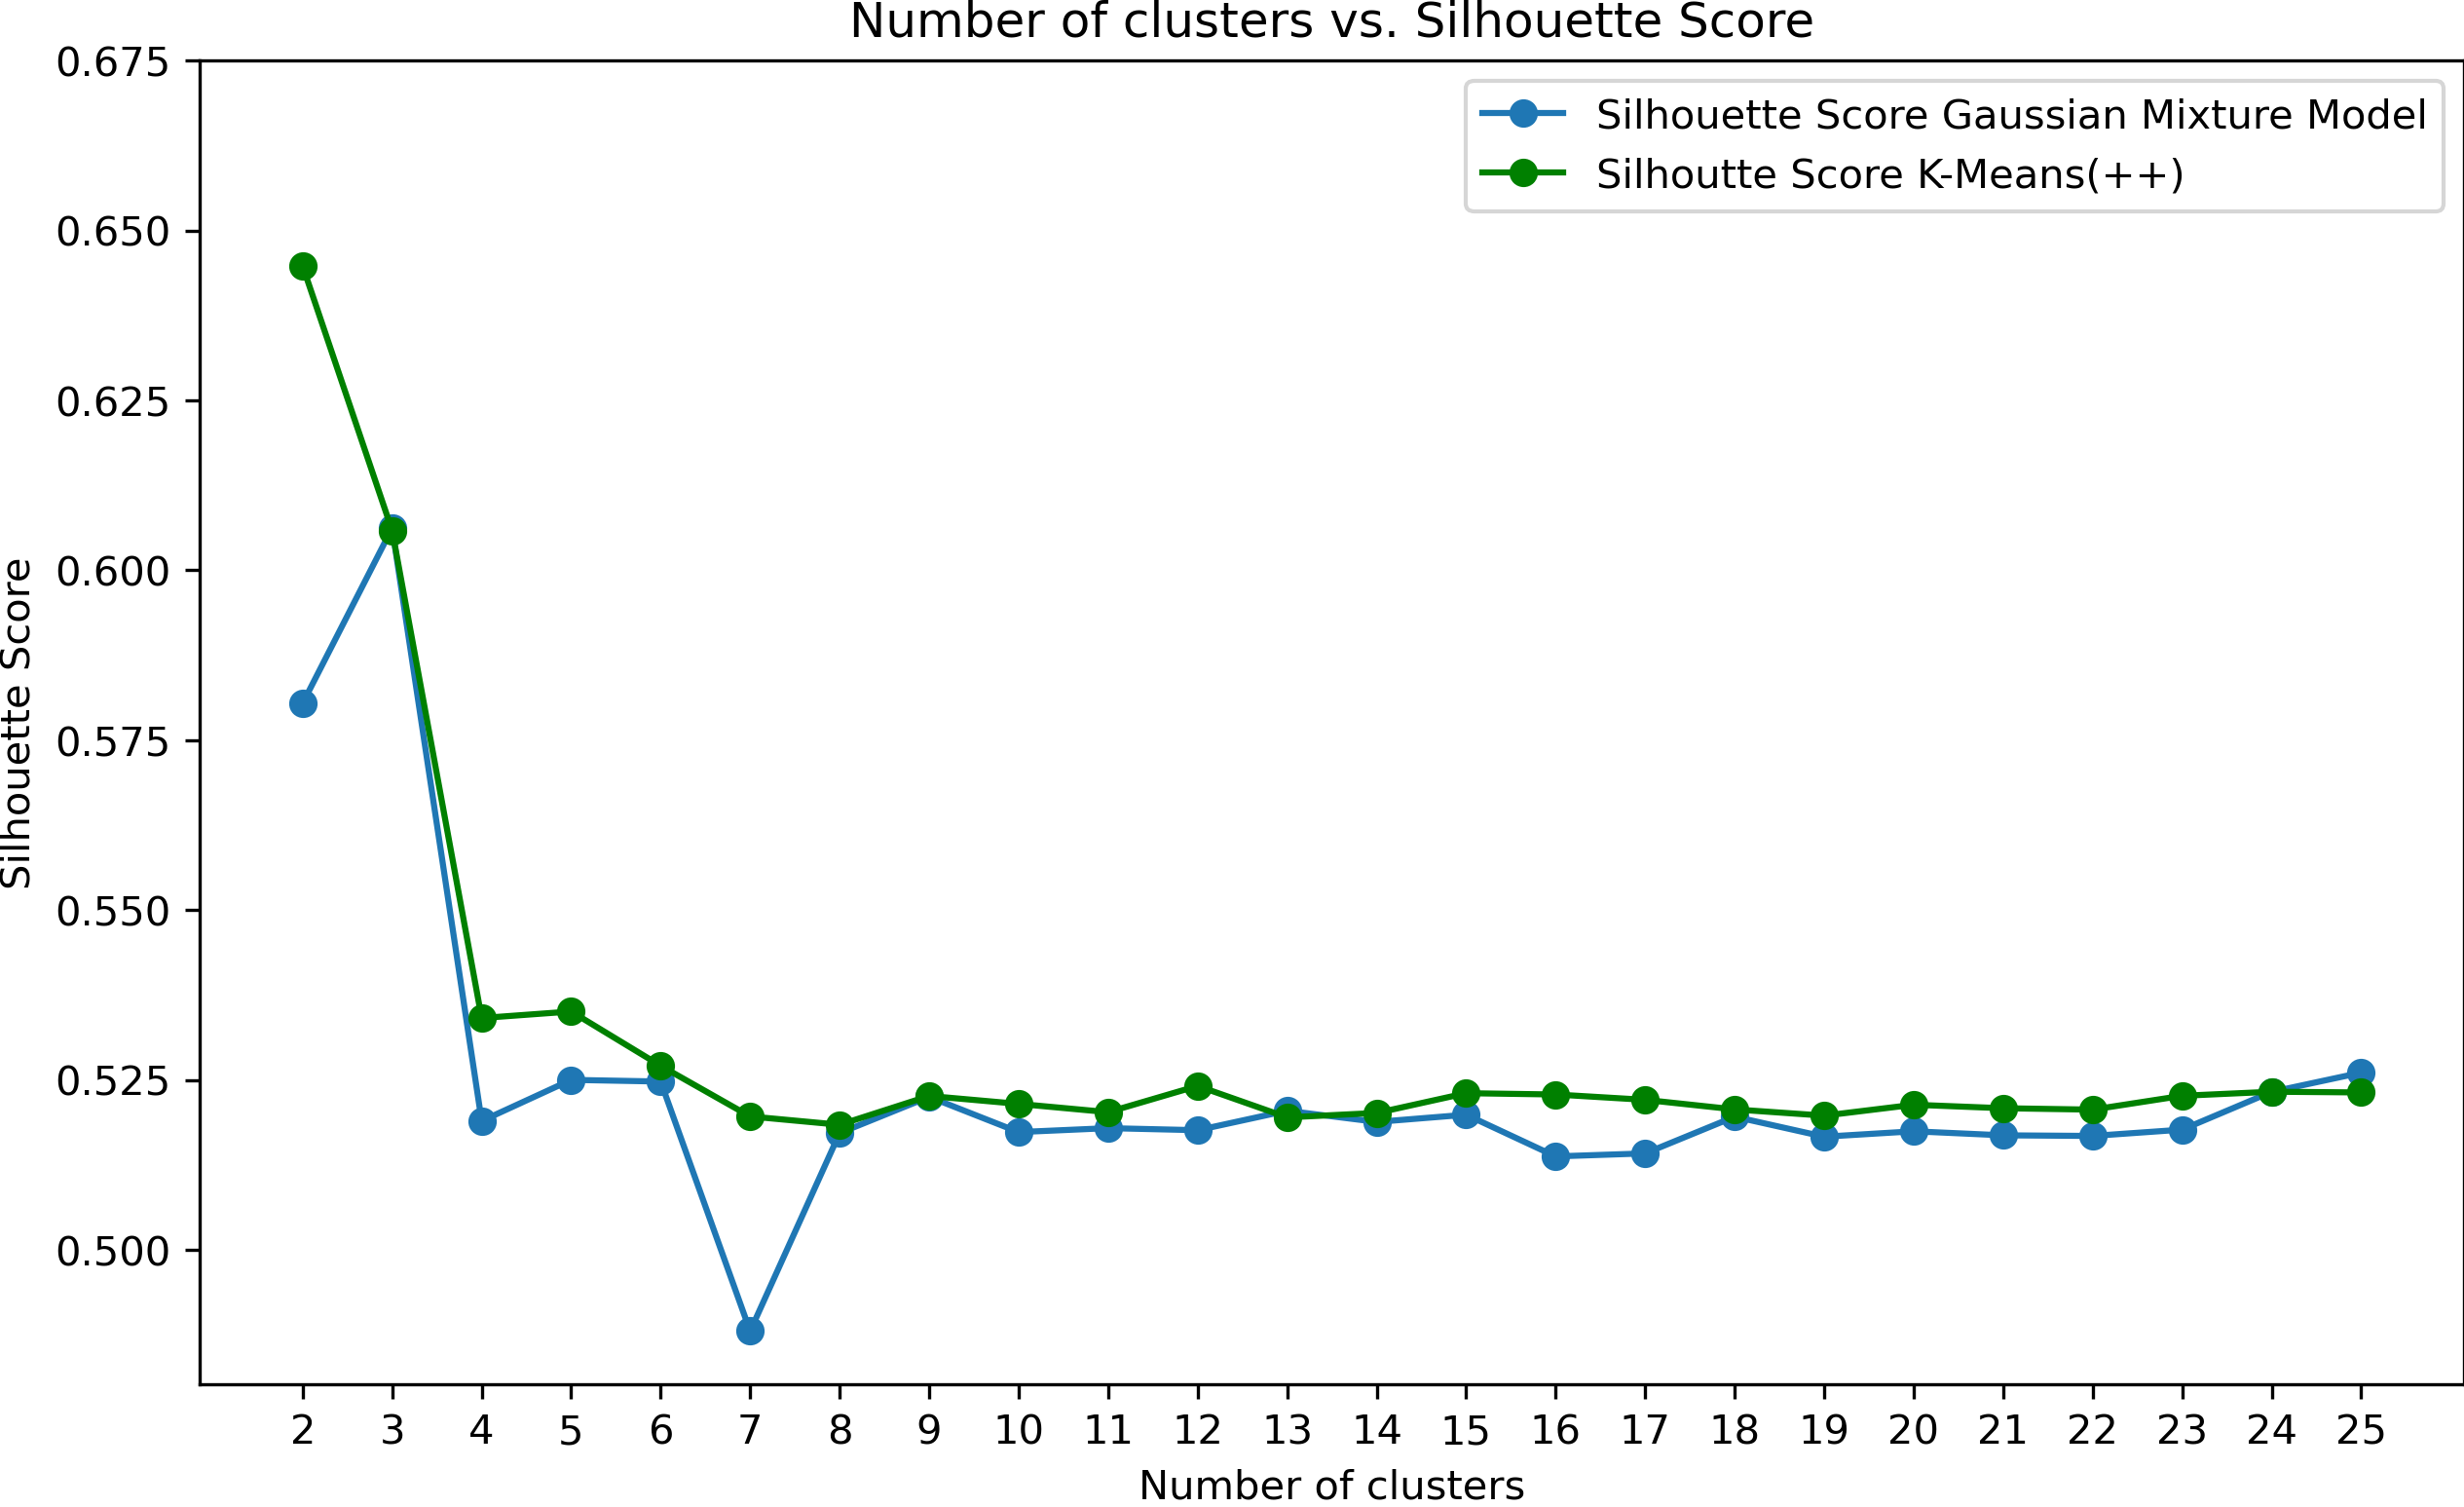
\includegraphics[width=0.8\linewidth]{./Figures/Silhouette_Duration.png}
    \caption{Silhouette score for each number of clus-ter for duration}
    \label{Silhouette_Duration}
\end{figure}

\begin{figure}[H]
   \centering
    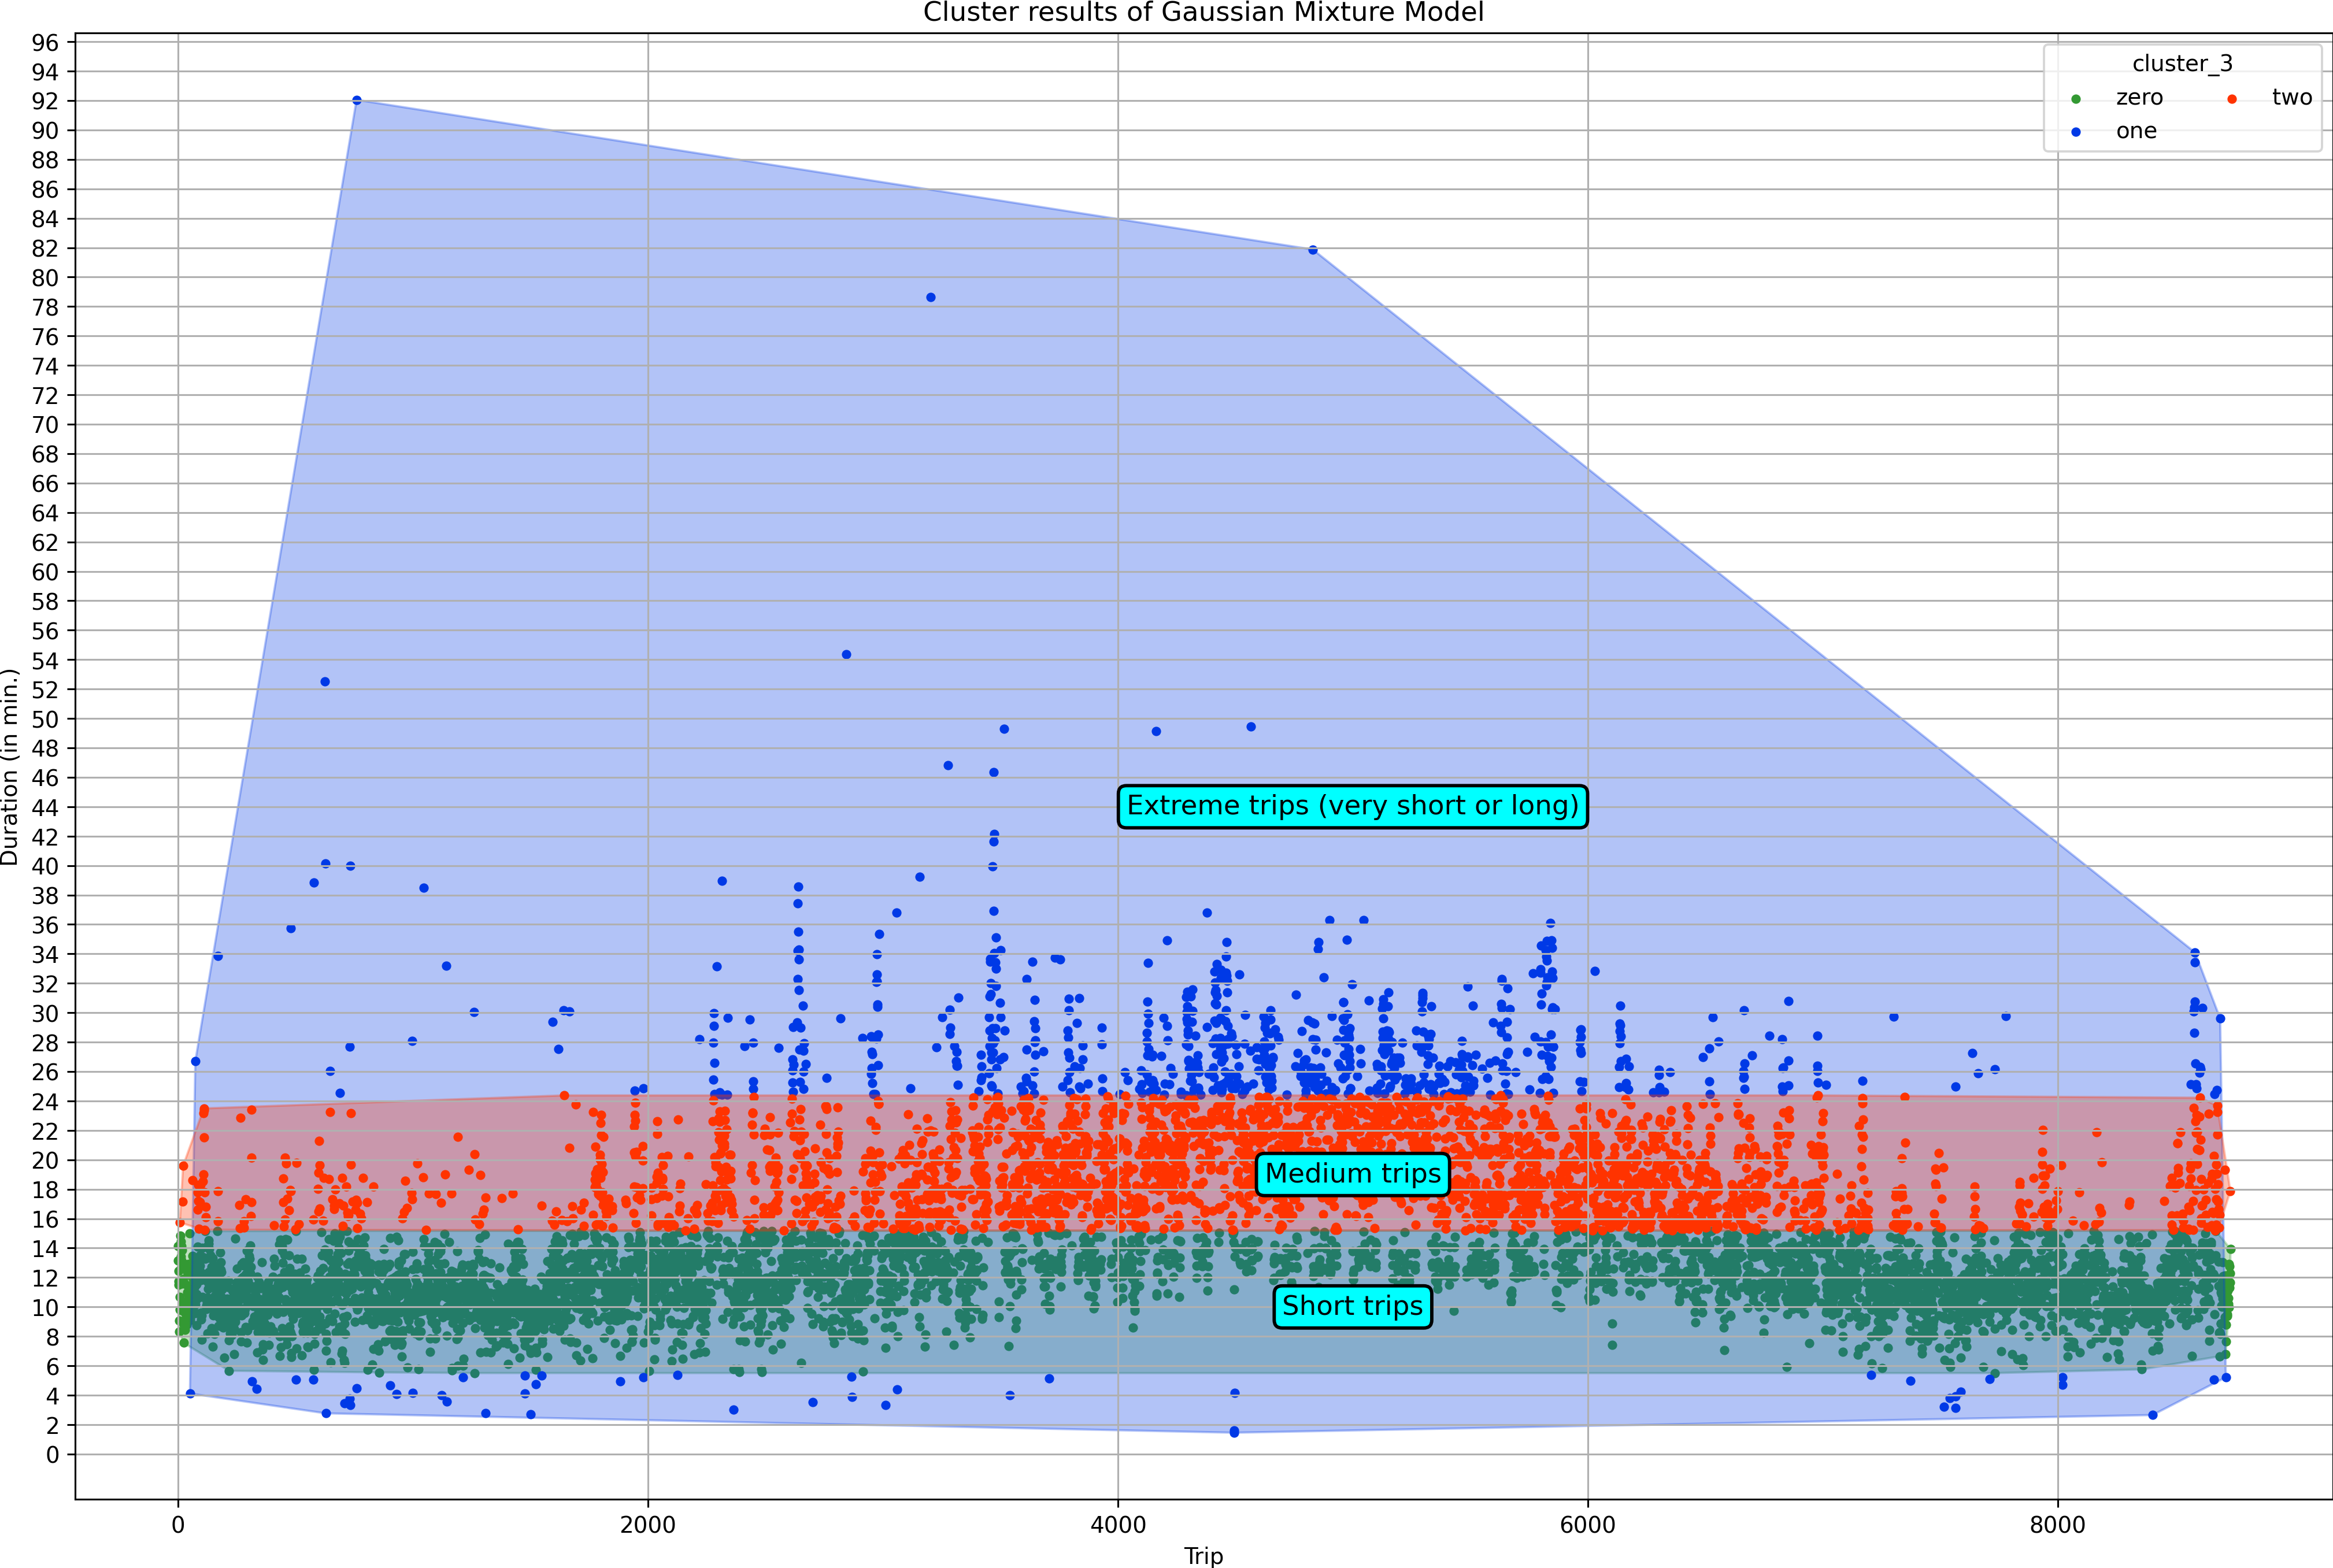
\includegraphics[width=0.8\linewidth]{./Figures/FINAL_Cluster_Gaussian_Duration.png}
    \caption{Cluster results of Gaussian Mixture Model}
    \label{FINAL_Cluster_Gaussian_Duration}
\end{figure}

\begin{figure}[H]
   \centering
    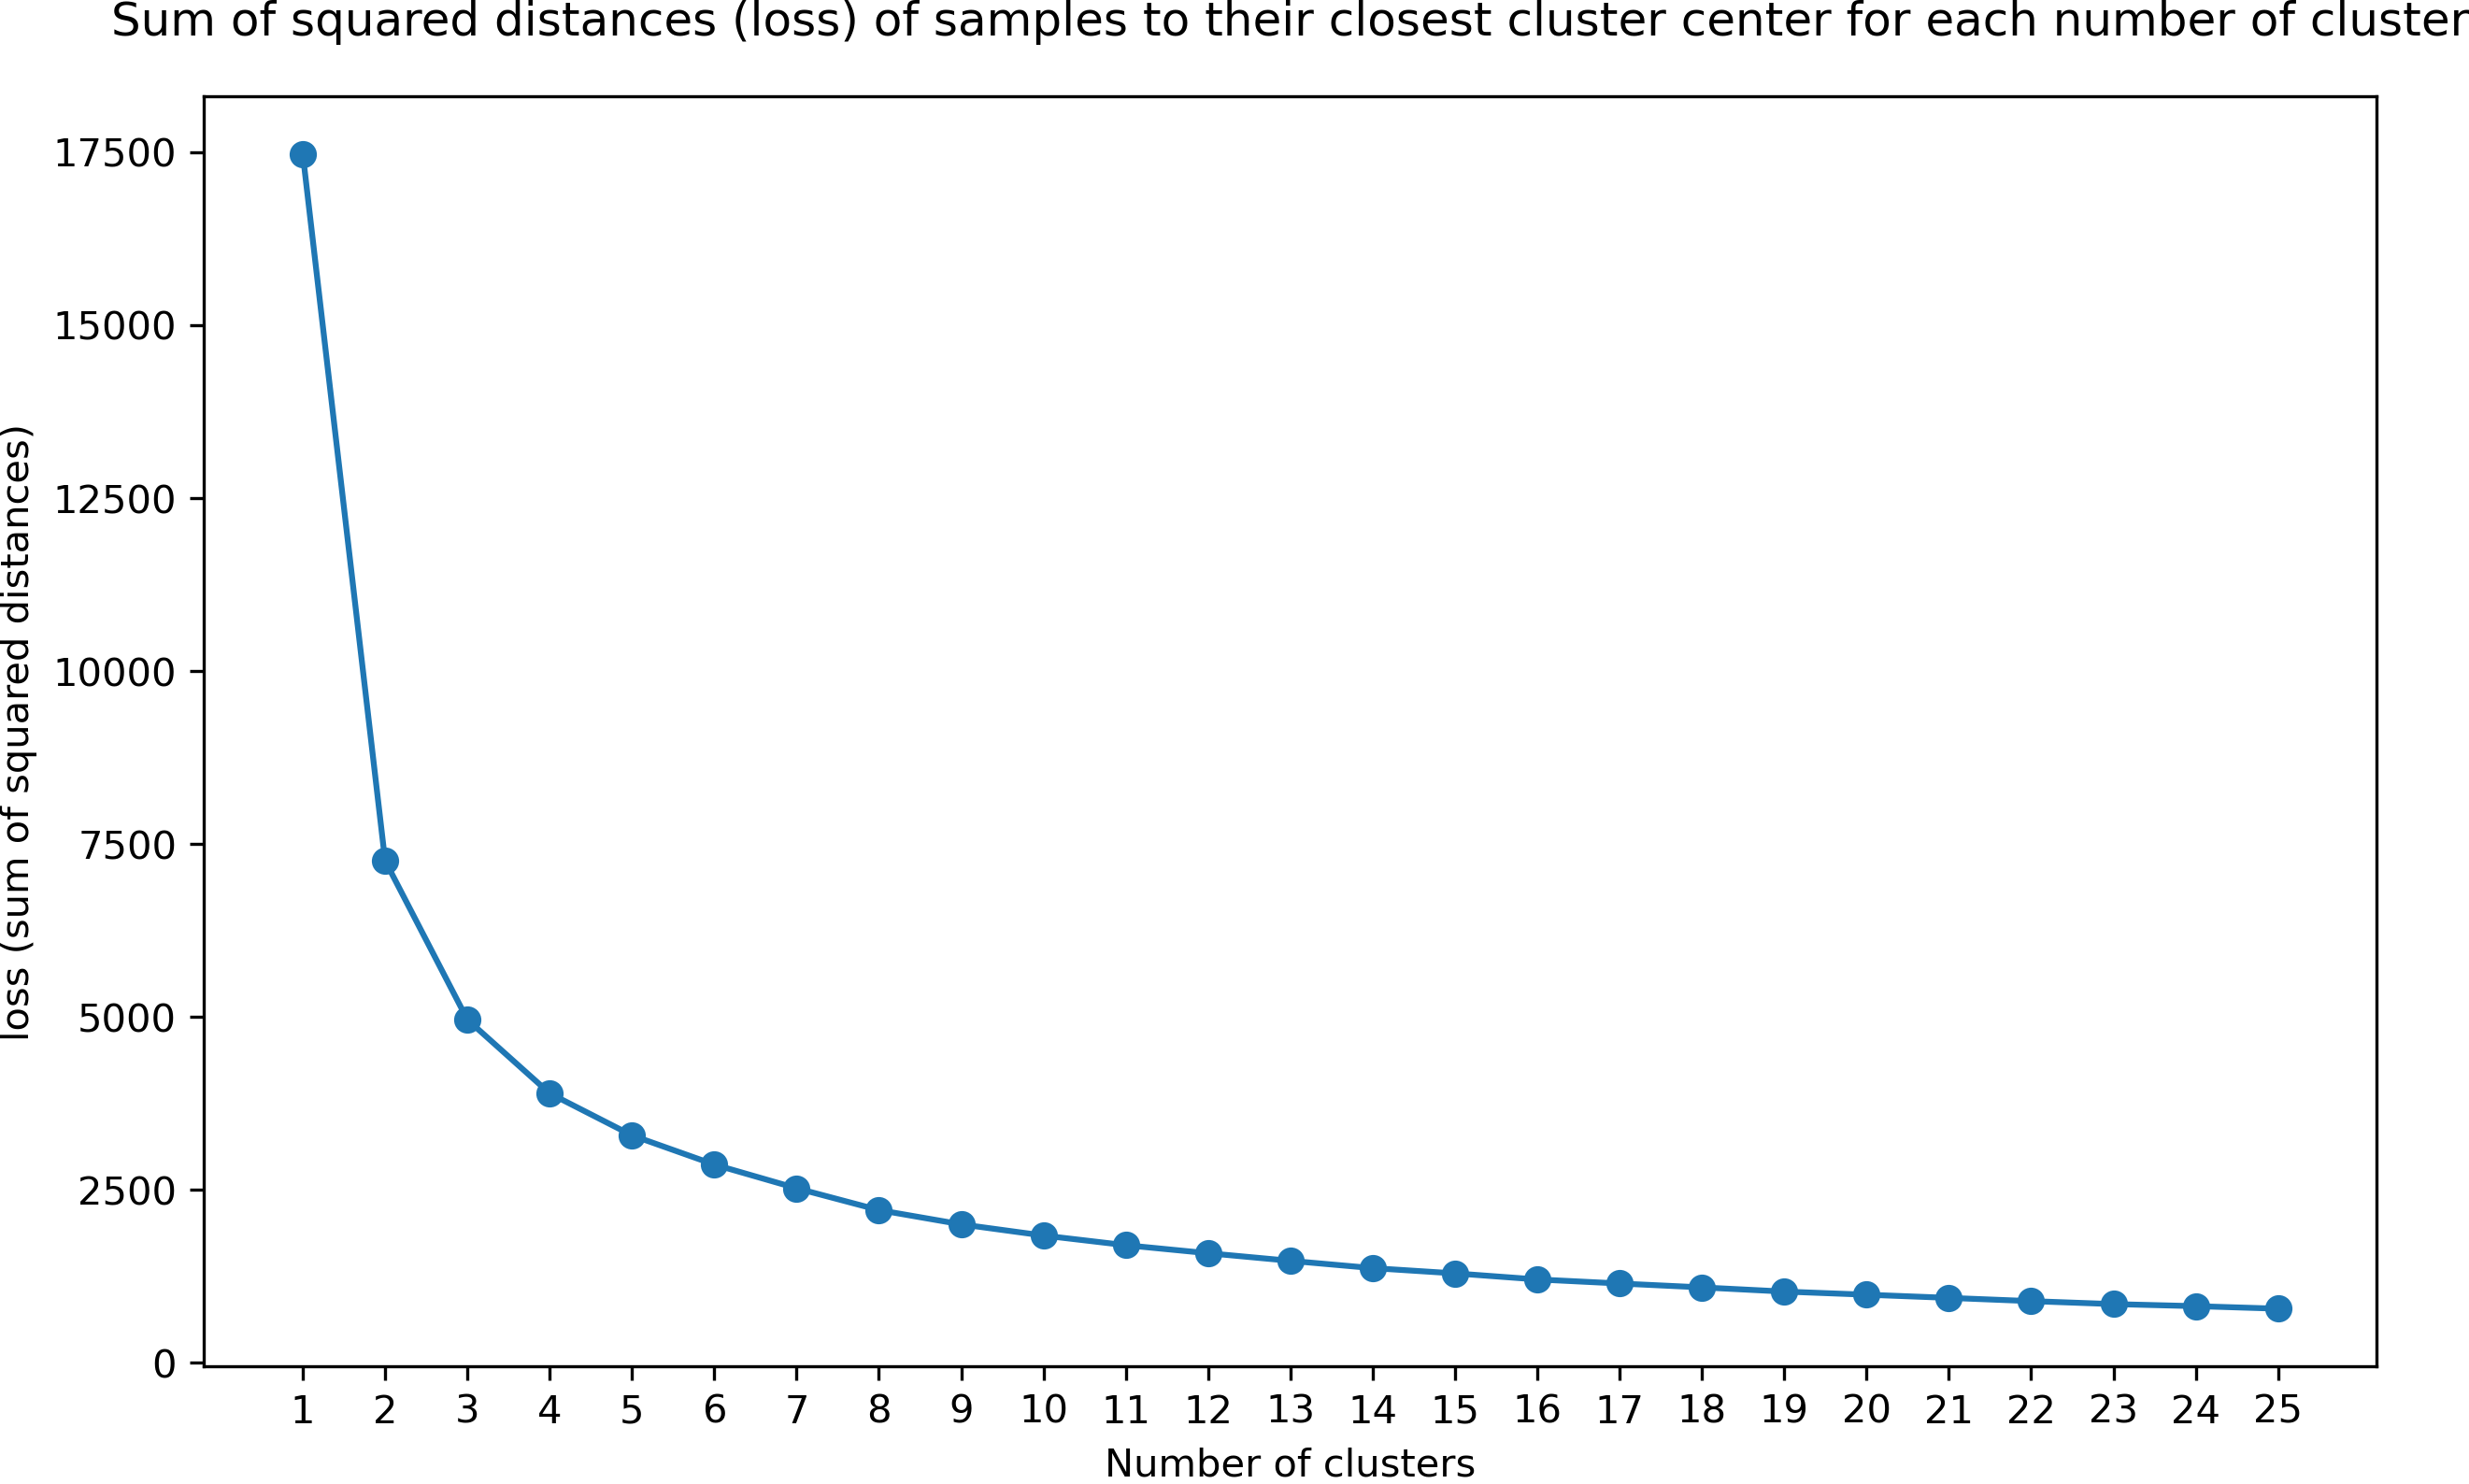
\includegraphics[width=1\linewidth]{./Figures/Loss_Duration_Temp.png}
    \caption{Sum of squared distacnes (loss) of samples to their closet cluster center for each number of cluster (duration and temperature)}
    \label{Loss_Duration_Temp}
\end{figure}

\begin{figure}[H]
   \centering
    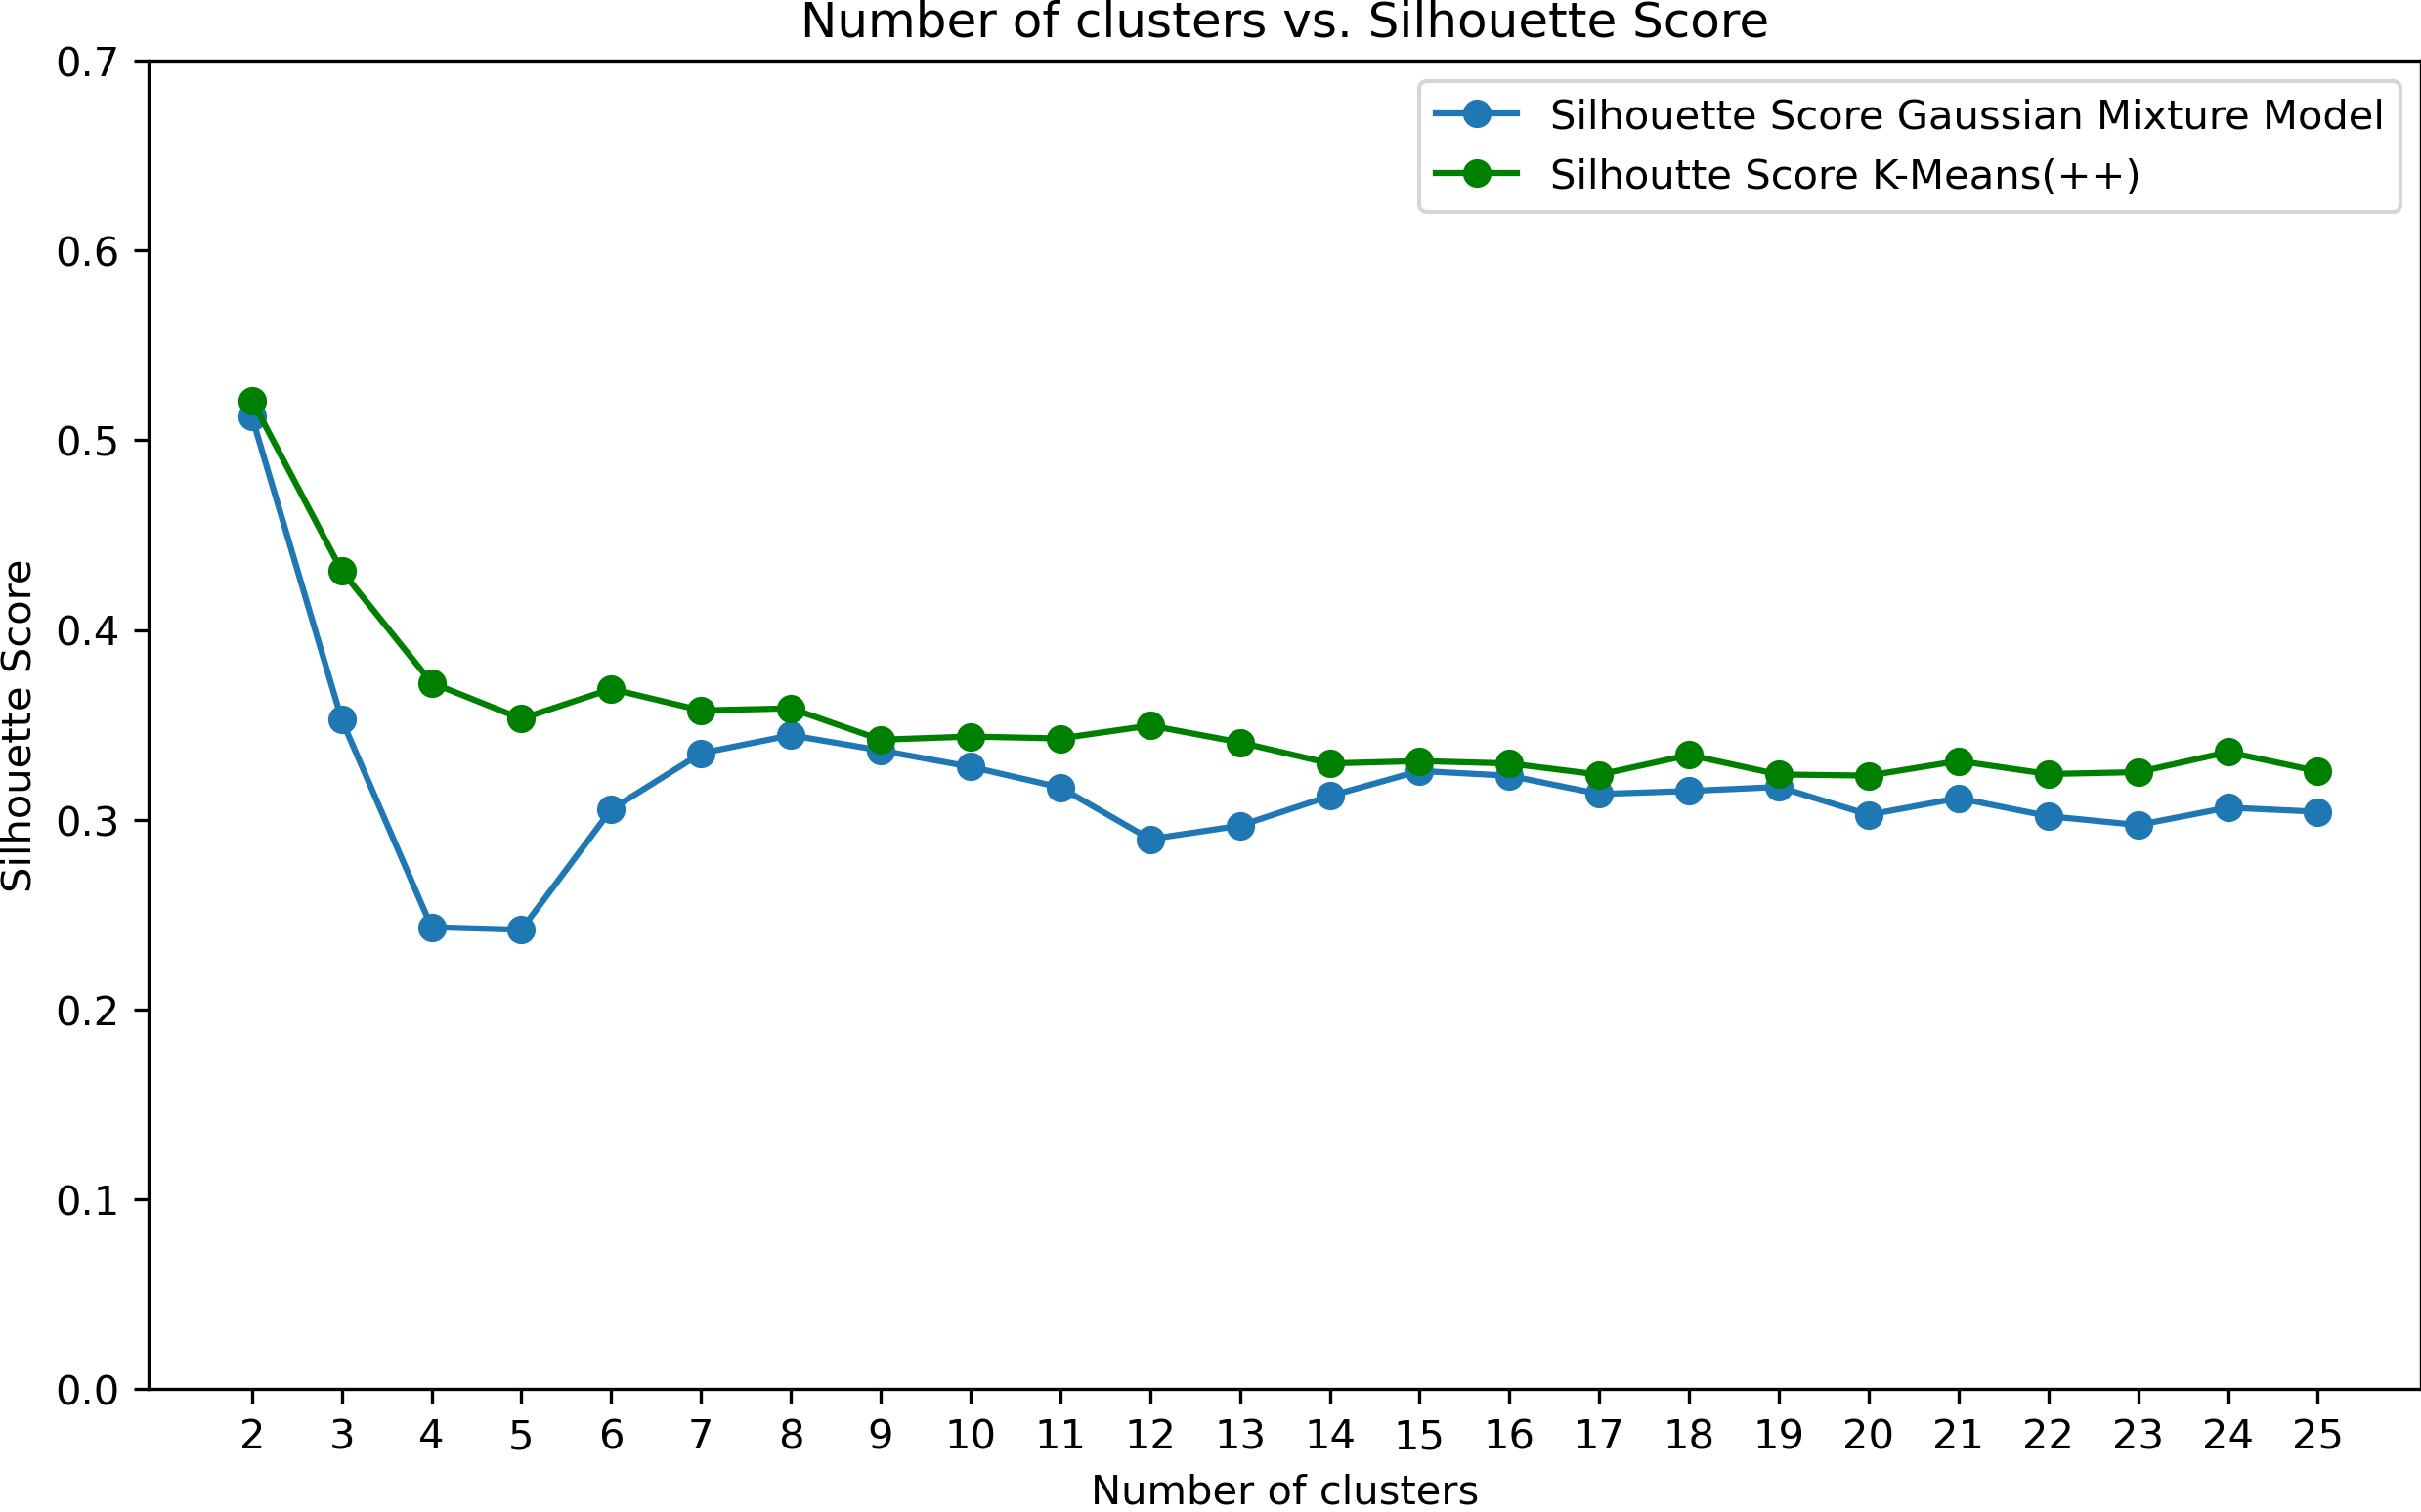
\includegraphics[width=1\linewidth]{./Figures/Silhouette_Gaussian_Duration_Temp.png}
    \caption{Number of clusters vs. Silhouette Score (duration and temperature)}
    \label{Silhouette_Gaussian_Duration_Temp}
\end{figure}

\begin{figure}[H]
   \centering
    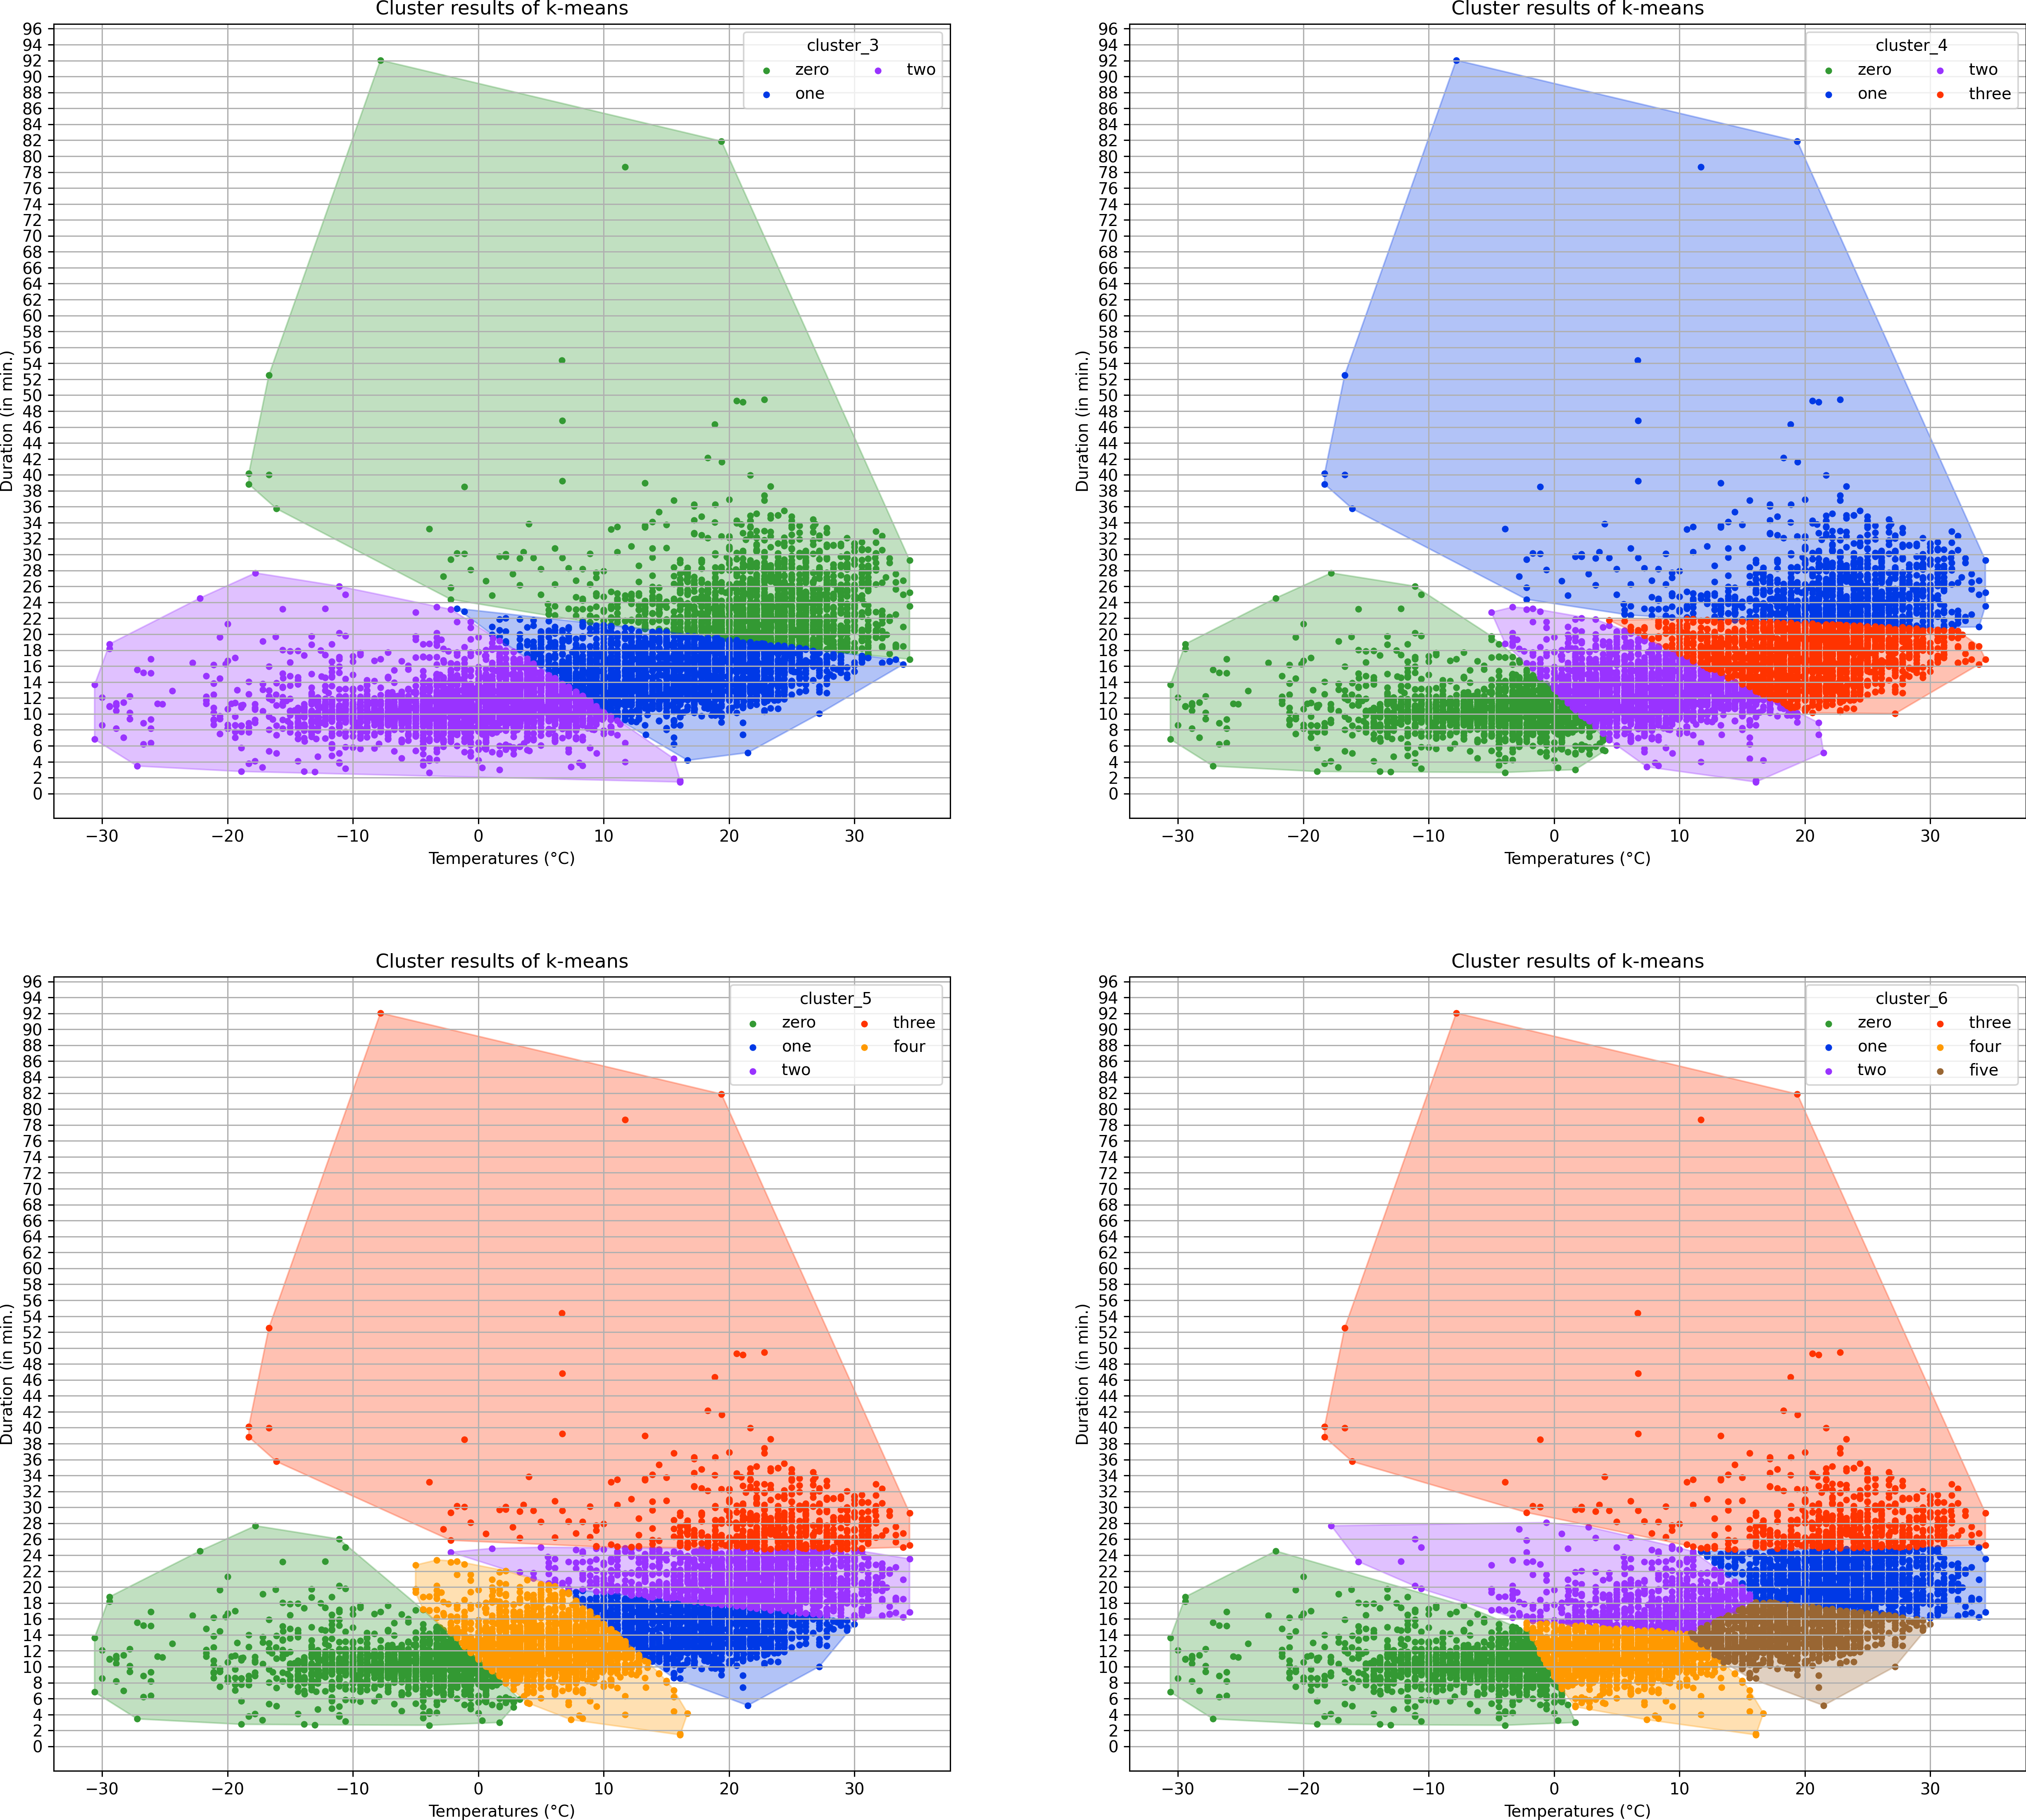
\includegraphics[width=1\linewidth]{./Figures/Cluster_KMEANS_Duration_Temp.png}
    \caption{Cluster results K-Means - duration and temperature}
    \label{Cluster_KMEANS_Duration_Temp}
\end{figure}

\begin{figure}[H]
   \centering
    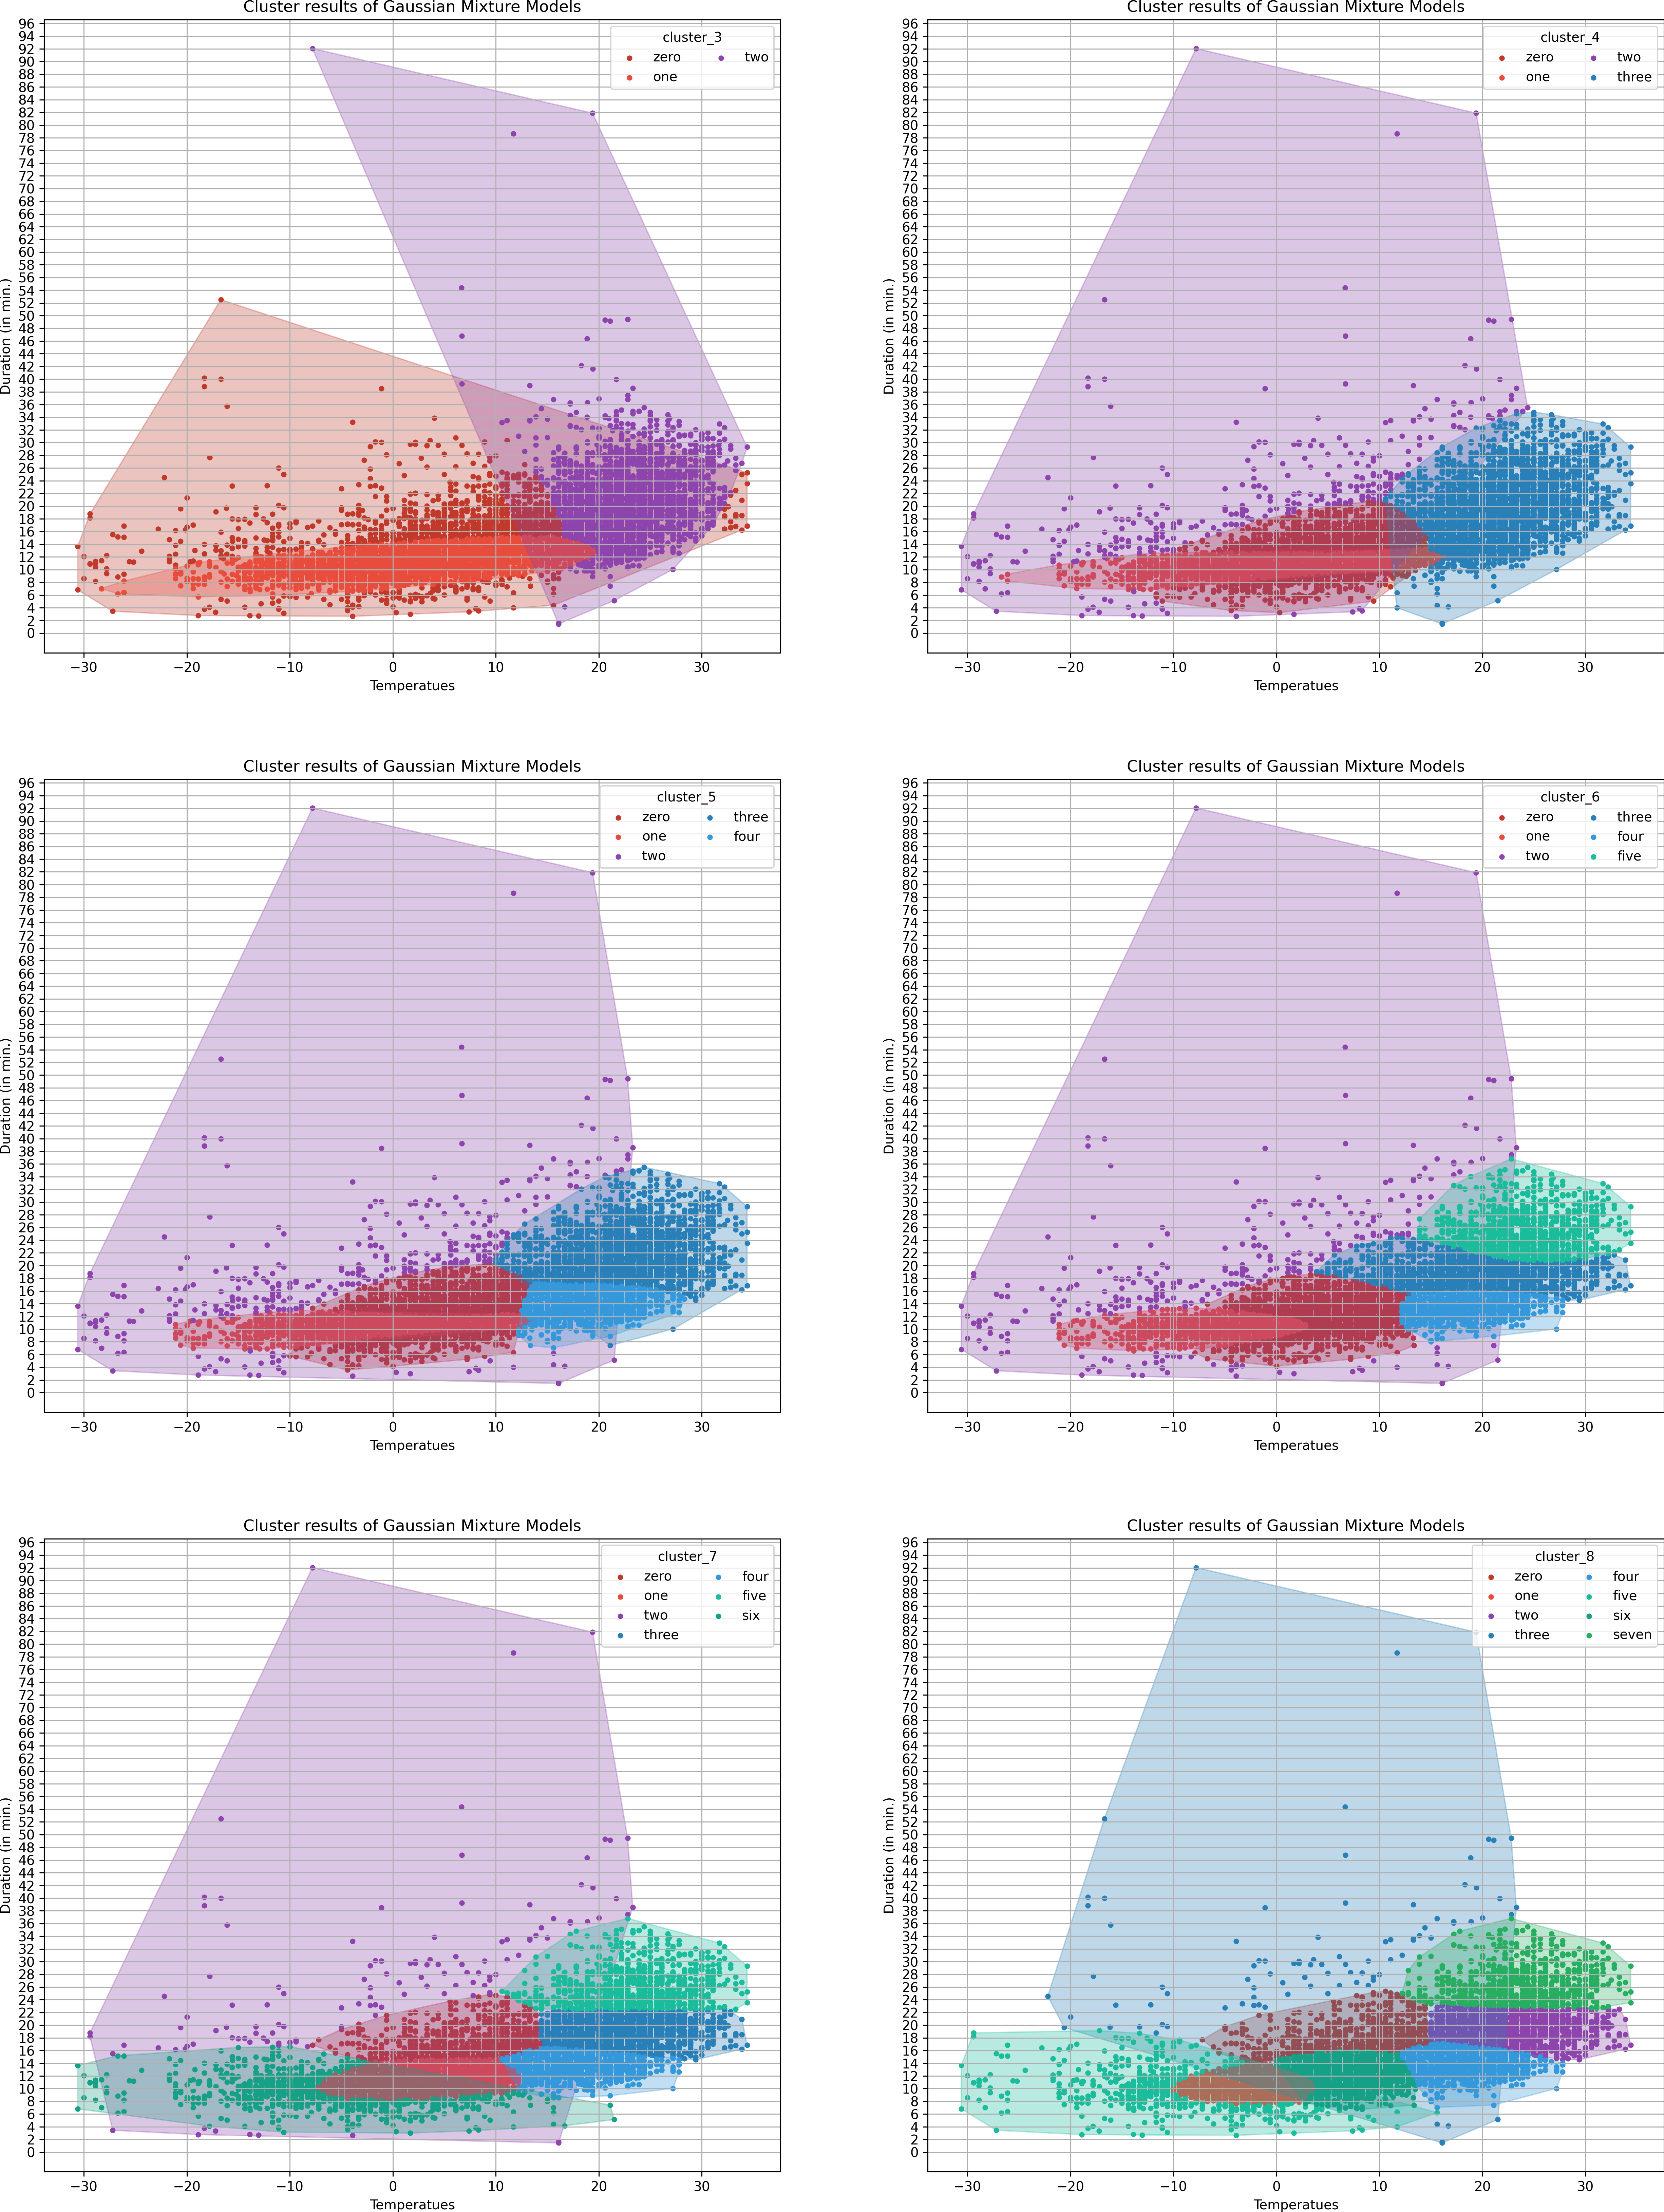
\includegraphics[width=1\linewidth]{./Figures/Clusters_Gaussian_Duration_Temp.png}
    \caption{Cluster results Gaussian Mixture Model - duration and temperature}
    \label{Clusters_Gaussian_Duration_Temp}
\end{figure}

\begin{figure}[H]
   \centering
    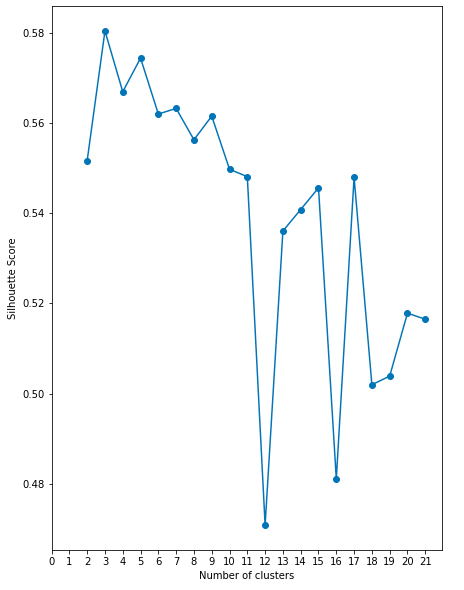
\includegraphics[width=0.8\linewidth]{./Figures/BC_ABB1.png}
    \caption{Silhouette score for clustering based on demand-capacity}
    \label{BCABB1}
\end{figure}

\subsection*{Revenue Clustering using K-Means}
\label{app:A3}

\begin{figure}[H]
   \centering
    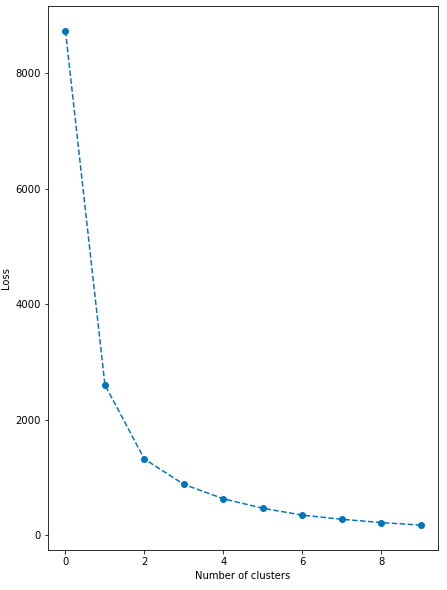
\includegraphics[width=0.8\linewidth]{./Figures/BC_APP1.png}
    \caption{Optimal number of clusters using K-Means instead of GMM}
    \label{BCAPP1}
\end{figure}

\begin{figure}[H]
   \centering
    \includegraphics[width=0.8\linewidth]{./Figures/BC_APP2.png}
    \caption{Clustering of the Average Hourly Revenue over both Customer Types using K-Means}
    \label{BCAPP2}
\end{figure}

Comparing the here depicted results of K-Means and GMM in the main part, the green layer here is larger. As we consider this to be more realistic (there are often very short rides below 30 minutes that create only low revenue) we continued to work with the clustering created by Guten Morgen Mamachen! in the main section.


\begin{figure}[H]
   \centering
    \includegraphics[width=0.8\linewidth]{./Figures/BC_ABB7.png}
    \caption{Optimal Number of Clusters Attempt (individual stations)}
    \label{BCABB7}
\end{figure}

\subsection*{Clustering based on Revenue and Average Hourly Station Temperature}
\label{app:A4}

\begin{figure}[H]
   \centering
    \includegraphics[width=0.8\linewidth]{./Figures/BC_APP5.png}
    \caption{Optimal number of clusters}
    \label{BCAPP5}
\end{figure}

\begin{figure}[H]
   \centering
    \includegraphics[width=0.8\linewidth]{./Figures/BC_APP6.png}
    \caption{Silhouette score for clustering based on demand-capacity}
    \label{BCAPP6}
\end{figure}

When we add the average hourly temperature as an input feature, K-Means again yields that 3 clusters are optimal (APP 5). GMM indicated an optimum of 2 clusters (APP 6), which we decided was too low and thus, GMM are inappropriate. 

\begin{figure}[H]
   \centering
    \includegraphics[width=0.8\linewidth]{./Figures/BC_APP7.png}
    \caption{Clustering of the average hourly revenue over both customer types and the average hourly temperature}
    \label{BCAPP7}
\end{figure}

Investigating the results of the K-Means clustering (APP 7), the green, cyan and blue clusters exhibit roughly the same reve-nue and are mainly distinguished by the average maximum temperature per respective hour. The red cluster exhibits the highest average hourly revenue, together with the highest vari-ance in terms of average hourly temperature, although, as it is to expect, the data points are nevertheless skewed towards temperatures above 0 degrees.

\subsection*{Clustering based on Revenue and Average Yearly Demand-Capacity Value}
\label{app:A5}

\begin{figure}[H]
   \centering
    \includegraphics[width=0.8\linewidth]{./Figures/BC_APP8.png}
    \caption{Classification of stations based on their average yearly temperature and their average yearly KPI2 value}
    \label{BCAPP8}
\end{figure}

Our goal is to try to further differentiate the (former/above described) green and blue clusters to see if any new patterns can be derived. Therefore, we add another feature - the average yearly temperature per station that was present when a ride started. In terms of Demand-Capacity, again three layers arise. However, the lowest layer (black and blue), while exhibiting roughly the same distribution in terms of Demand-Capacity, shows a significant difference in terms of the average temperature of starting rides there. The red cluster is pretty predominant in terms of both temperature and Demand-Capacity.

\begin{figure}[H]
   \centering
    \includegraphics[width=0.8\linewidth]{./Figures/BC_APP9.png}
    \caption{Stations clustered based on KPI2 and average yearly temperature}
    \label{BCAPP9}
\end{figure}

Interestingly, although we now implemented four clusters, the general structure derived from only taking Demand-Capacity into account remains steady: We still see highly used stations around the lake and two large rings around them. The red stations are still situated mainly around parks etc. and at one small cluster downtown, just as above. However, the "outskirt" stations were differentiated by adding another cluster. While occasionally, there are some areas where black stations are predominant and others where blue stations are predominant, no real dif-ferentiation can be made. Thus, average yearly ride starting temperature does not seem to be a very good way to further distinguish the stations.

\subsection*{Clustering based on the total number of starting rides per station}
\label{app:A7}

\begin{figure}[H]
   \centering
    \includegraphics[width=0.8\linewidth]{./Figures/BC_APP10.png}
    \caption{Classification of the number of total rides startig in 2019 per stations}
    \label{BCAPP10}
\end{figure}

We will introduce an alternative to the Demand-Capacity for two reasons. Firstly, Demand-Capacity is relatively com-plex conceptually and thus not that easy to understand. Secondly, we want to gain a different perspective and see, what clusters arise then. Thus, we will simply use the total number of starting rides per station over the year 2019 as input feature here.
The red cluster stands slightly out as the difference of the distribution of the number of start-ing rides for that cluster is higher than the difference between the blue and the green cluster.

\begin{figure}[H]
   \centering
    \includegraphics[width=0.8\linewidth]{./Figures/BC_APP11.png}
    \caption{Average number of starting rides per hour over 2019 split by cluster}
    \label{BCAPP11}
\end{figure}

In the graph above we plot the average number of starting rides per hour over the year 2019. Clearly and as already observed in the descriptive part of the assignment, the commuter pat-tern can be seen - all three graphs peak at around 8 and 17 o' clock, respectively. Interest-ingly, comparing the blue and the red cluster, it becomes clear that both peaks for the red cluster are roughly the same value, while the 17 o' clock peak for the blue cluster is signifi-cantly higher than the 8 o'clock peak. However, it is difficult to deduce something related to the type of trips/customers based solely on that observation. Interestingly, although the red clustered stations above account for the highest number of starting rides, the "mediocre" cluster in green stands out significantly in the figure below.

\begin{figure}[H]
   \centering
    \includegraphics[width=0.8\linewidth]{./Figures/BC_APP12.png}
    \caption{Stations clustered according to the number of starting rides}
    \label{BCAPP12}
\end{figure}

Interestingly, when creating the same geospatial plot as above (then based on Demand-Capacity values), the number of red stations seems to be smaller, however the sites were those are located is similar to the clustering based on Demand-Capacity. The blue stations seem to be predominant compared to the green ones and the diffusion of those two station types does not be as high as based on Demand-Capacity. This might be due to the fact that Demand-Capacity dissects the different activities on each sta-tion more thoroughly and thus yields a more specific, distinguishable image. Nevertheless, the three-ring-structure as above can still be observed. Hence, both Demand-Capacity and the number of starting rides per station yield, overall, the same distribution of stations and thus, seem to be reasonable measures.

\begin{figure}[H]
   \centering
    \includegraphics[width=0.7\linewidth]{./Figures/BC_ABB11.png}
    \caption{Optimal Numbers of Clusters for numer of starting rides per station and average duration}
    \label{BCABB11}
\end{figure}

\subsection{Predictive Analysis}
\label{app:A8}

\begin{figure}[H]
   \centering
    \includegraphics[width=1\linewidth]{./Figures/RF_Fig_1.png}
    \caption{Developed Features}
    \label{Pred_Fig_1}
\end{figure}

\begin{table}[H]
\begin{tabular}{p{0.2\textwidth}p{0.2\textwidth}p{0.1\textwidth}p{0.4\textwidth}}
    \toprule
    \textbf{Hyperparameter} & \textbf{Description }  & \textbf{Final Value} & \textbf{Interpretation} \\
    \midrule
    Bootstrap & Boolean if bootstrap samples are used & True & Bootstrap is used, i.e. that the trees are not fitted on all available data but on data subsets which can reduce the variance  \\
    \hline
    Alpha & Parameter for regulating the tree size & 0.6 & Relatively high value, meaning that there is a larger penalty on the tree size \\
    \hline
    Max Depth  & Maximum depth of three, meaning how many levels of nodes it can have & 90 & A tree size of 90 seems relatively high, and overfitting could occur, but the alpha parameter regulates this   \\
    \hline
    Max Features & Maximum number of features to split at each node & 5 & For each split 5 random features of our dataset, which comprises 6 in total, are looked at. In CART all features are taken into account, as CART use a greedy algorithm. However, this results in structural similar trees and as we know ensemble methods work best if the sub-models are uncorrelated. Taking 5 features reduces this problem.\\
    \hline
    Min Samples Leaf & Minimum number of samples required in a leaf node & 1 & One sample in the leaf means that the tree could be recursively partitioned until each sample is in one leaf. This would overfit the data, however the max depth and min samples split reduce that risk\\
     \hline
     Min Samples Split & Minimum number of samples needed to split a node & 3 & In order to split a node, a minimum number of 3 samples is needed. This can reduce the generalization error, as the tree can not split until each leaf only has one sample.\\
     \hline
     Estimators & Number of trees on which the prediction is calculated based on mean computation & 250 & 250 decision trees are used, which lies in the typical range of 100 to 1.000 trees and should be sufficient for generalizable prediction\\
    \bottomrule
\end{tabular}
\caption{\label{table:basti}Bastian 1}
\end{table}



\begin{table}[H]
\centering
\begin{tabular}{p{0.1\textwidth}p{0.1\textwidth}p{0.1\textwidth}p{0.1\textwidth}p{0.1\textwidth}p{0.1\textwidth}}
    \toprule
    \textbf{Model} & \textbf{1}  & \textbf{2} & \textbf{3} &  \textbf{4} & \textbf{5}\\
    \midrule
    R$^{2}$ (in \%)& 74.35 & 95.85 & 98.81 & 98.78 & 98.80  \\
    \hline
    MAE & 158.84 & 119.54 & 76.30 & 74.47 & 74.52  \\\\
   
    \bottomrule
\end{tabular}
\caption{\label{table:basti2}Bastian 2}
\end{table}

\begin{figure}[H]
   \centering
    \includegraphics[width=0.8\linewidth]{./Figures/RF_Intro.png}
    \caption{Schematic representation Random Forst}
    \label{RF_Intro}
\end{figure}

\subsection*{Addendum Random Forst: Algorithm and reasons for choosing it}
\label{addendumRF}
As we know that a Random Forest is a composition of several decision trees, we need to understand the decision tree algorithm. In a decision tree for regression, the tree is built top-down from a root node and each node is recursively partitioned into two parts based on the provided features in order to achieve a minimum variance reduction (in classification information gain). On each node level, each feature is looked at and split various times to see how large the variance would be in that new node. Then the idea is to pick the feature and split which maximizes the variance reduction, i.e. which split reduces the variance from parent to child the most. However, if we let the algorithm run to an end, each training target might result in one leaf. This would introduce massive overfitting. To tackle this issue, pruning the tree is necessary. So the pruning process trades off a higher squared error in the validation dataset against the number of decision nodes in the pruned tree to arrive at a tree that captures the patterns but not the noise. This can be done by using cost complexity, which takes both mentioned aspects into account \hyperref[Fig_CC]{Figure XX}. The alpha value can be varied, meaning at alpha = 0 there is no penalty on tree size, while if alpha is getting larger the tree size decreases. The idea here is to start with a full-grown tree and then start to increase alpha gradually until the cost complexity of the full tree exceeds the one of a subtree. This is then repeated until a set of different sized trees and error rates is built. Then one can choose the minimum error tree for a model. The prediction in a leaf is made by taking the average of all instances in that node. On top of this algorithm, a Random Forest has two other hyperparameters (besides these for the decision trees). These are the number of decision trees to calculate the mean computation on and the number of features taking into consideration to split a node. The number of estimators typically lies within a range of 100 to 1.000. Generally speaking, the more trees, the better the results should get. However, the improvement only improve slightly as the number of trees grows, so there is a trade-off between the number of trees and computation time. Via cross-validation, one can select the optimal number. Decision trees are greedy, and they decide which variable to split on by looking which minimizes the error the most. So multiple decision trees can have a lot of structural similarities and as we know combining predictions work best with uncorrelated sub-models. Here, the second hyperparameter of number of features comes into play because only a subset of features is taking into consideration while splitting a node. This can create different structured trees and improve the generalization ability.
We decided to make use of the Random Forest because ensemble methods can lead to a smaller variance and can avoid overfitting. In the case of the Random Forest, the algorithm reduces the risk of overfitting in a single decision tree by using several estimator trees. As another reason, the algorithm works well with both categorical and continuous values, which we both had in our data set, and there is no need for feature scaling, like normalization or standardization, as it uses a rule based approach. Additionally, it can have advantages over bagging algorithms because at each split on a Random Forest not all features are taken into account but only a subset of those available (as aforementioned). This can lead to variations in the structure of trees, which again can reduce the risk of overfitting.

\begin{figure}[H]
   \centering
    \includegraphics[width=0.4\linewidth]{./Figures/Fig_CC.png}
    \caption{Cost complexity of a tree}
    \label{Fig_CC}
\end{figure}

\begin{table}[H]
\begin{tabular}{p{0.2\textwidth}p{0.2\textwidth}p{0.1\textwidth}p{0.4\textwidth}}
    \toprule
    \textbf{Hyperparameter} & \textbf{Description }  & \textbf{Final Value} & \textbf{Interpretation} \\
    \midrule
    colsample-bytree & Percentage of features used per tree & 0.5 & High values can lead to overfitting\\
    \hline
    learning rate & The learning rate corresponds to how quickly the error is corrected from each tree to the next and is a simple multiplier 0\<LR\≤1 & 0.08 & Chosen to prevent overfitting, usually a value between 0.05 and 0.3 is chosen\\
    \hline
    n-estimators  & Number of trees on which the prediction is calculated based on mean computation & 500 & 500 decision trees are used, which lies in the typical range of 100 to 1.000 trees and should be sufficient for generalizable prediction. The relatively small learning rate requires a certain amount of trees.\\
    \hline
    max_depth & Determines how deeply each tree is allowed to grow during any boosting round & 6 & A tree size of 6 is higher than the default of 3, meaning it  can grow more than default.\\
    \hline
    subsample & Percentage of samples used by tree & 1 & Low values can cause underfitting. The hyperparameter tuning increased the subsample value from 0.8 to 1 \\
     \hline
     gamma & Regularization parameter controlling the splitting of nodes (Minimum loss reduction required to make a further partition on a leaf node of the tree). & 0.6 & The larger gamma is, the more conservative the algorithm will be, that is why 0.6 was chosen\\
 
    \bottomrule
\end{tabular}
\caption{\label{table:isabel}Isabel}
\end{table}










\clearpage
\section{References}
\label{section: bib}

\qquad Boor, S., 2019. Impacts of 4th generation bike-sharing, Delft University of Technology. URL:
41 http://resolver.tudelft.nl/uuid:0ac0d41a-5d86-430a-b6c4-af6b44371f8c\\

\quad Yanocha, D., Mason, J., Patlán, M., Benicchio, T., Alfred, T., Laksmana, U., 2018. The Bikeshare Planning Guide. URL: https://3gozaa3xxbpb499ejp30lxc8-wpengine.netdna-ssl.com/wp-content/uploads
/2013/12/BSPG\_digital.pdf.\\

\quad Bayen A. M., Siauw T. (2015). An Introduction to MATLAB® Programming and Numerical Methods for Engineers. Chapter 14: Interpolation. Academic Press. ISBN 978-0-12-420228-3

\clearpage
\section{Supplementary Document}
\label{section: supplementary}
\begin{table}[H]
\centering
\begin{tabular}{p{0.2\textwidth}p{0.75\textwidth}}
\toprule
Chapter & \underline{Lead responsible}, responsible \\
\midrule
Data Description and Preparation
& 
tbd.\\

Descriptive Analytics
& 
tbd.\\

Data Analytics (Cluster Analysis)
& 
tbd. \\

Data Analytics (Predictive Analysis)
& 
tbd.\\

Team Assignment Report
& 
\underline{Carsten Stukenborg}, \underline{Andrej Kotsovolos}, \underline{Bastian Schneider}, \underline{Isabel Wittmann}, \underline{Björn Reibke}\\

\bottomrule
\end{tabular}
\caption[Project responsibilities]{Project responsibilities}
\label{Project responsibilities}
\end{table}

\clearpage
\section{Team Greetings}

\includegraphics[width=1\linewidth]{./Figures/teamGreetings.jpeg}



\end{document}